%\documentclass{gen-m-l}
\documentclass[12pt,letterpaper,oneside,titlepage]{article}
\usepackage[latin1]{inputenc}
\usepackage{amsmath}
\usepackage{amsfonts}
\usepackage{amssymb}
\usepackage{graphicx}
%\usepackage{geometry}
%\geometry{letterpaper, portrait, left=.5in, right=.5in , top=.2in , bottom= .5in ,includefoot}
\usepackage[letterpaper, portrait, margin=.2in , includefoot]{geometry}
\usepackage{lscape}
\usepackage{tikz}
\usetikzlibrary{matrix,calc}
\usepackage{color}
\usepackage{tabto}
\usepackage{pgfplots}
\pgfplotsset{compat=1.7}
\pgfplotsset{width=7cm,compat=1.13}%
\usepackage{lscape}
\usepackage{rotating}
\usepackage{pdflscape}
\usepackage{capt-of}

\usepackage{makeidx}
\makeindex
\usepackage[totoc]{idxlayout}
\usepackage{imakeidx}
%\usepackage[toc,page,header]{appendix}

\usepackage[page,toc,titletoc,title]{appendix}
\usepackage{tocloft}
\usepackage{blindtext}
\usepackage{animate}
\usepackage{enumitem}






\usepackage[pdftex,
pdfauthor={Scott ``Cash'' Fields},
pdftitle={Tio Cash 's Sort of Primes},
pdfsubject={Primes},
pdfkeywords={Find Primes},
pdfproducer={Latex with hyperref, TeXstudio},
pdfcreator={pdflatex, or other tool , TeXstudio}]{hyperref}
\usepackage{indentfirst}


\usepackage{attachfile}






\usepackage[]{hyperref}
%\hypersetup{
%%	pdftitle={Tio Cash 's Sort of Primes},
%%	pdfauthor={Scott \textbf{``Cash''} Fields},
%%	pdfsubject={Tio Cash's Sort of Primes},
%	%pdfkeywords={keyword1, keyword2},
%	bookmarks=true,         
%	bookmarksnumbered=true,     
%	bookmarksopen=true,         
%%	bookmarksopenlevel=6,       
%	colorlinks=true,   
%	allcolors=blue,        
%	pdfstartview=Fit,           
%	pdfpagemode=UseOutlines,    % this is the option you were lookin for
%%	pdfpagelayout=TwoPageRight
%}
%%%%%%%%%%%%%%%%%%%%%%%%%%%%
%%%%%%%%%%%%%%%%%%%%%%%%%%%%
%%%%%%%%% cube pile %%%%%%%%%%%%%
%\documentclass[parskip]{scrartcl}
%\usepackage[margin=15mm,landscape]{geometry}
%\usepackage{tikz}
\usepackage{keyval}
\usepackage{ifthen}
%====================================
%emphasize vertices --> switch and emph style (e.g. thick,black)
%====================================
\makeatletter
% Standard Values for Parameters
\newcommand{\tikzcuboid@shiftx}{0}
\newcommand{\tikzcuboid@shifty}{0}
\newcommand{\tikzcuboid@dimx}{3}
\newcommand{\tikzcuboid@dimy}{3}
\newcommand{\tikzcuboid@dimz}{3}
\newcommand{\tikzcuboid@scale}{1}
\newcommand{\tikzcuboid@densityx}{1}
\newcommand{\tikzcuboid@densityy}{1}
\newcommand{\tikzcuboid@densityz}{1}
\newcommand{\tikzcuboid@rotation}{0}
\newcommand{\tikzcuboid@anglex}{0}
\newcommand{\tikzcuboid@angley}{90}
\newcommand{\tikzcuboid@anglez}{225}
\newcommand{\tikzcuboid@scalex}{1}
\newcommand{\tikzcuboid@scaley}{1}
\newcommand{\tikzcuboid@scalez}{sqrt(0.5)}
\newcommand{\tikzcuboid@linefront}{black}
\newcommand{\tikzcuboid@linetop}{black}
\newcommand{\tikzcuboid@lineright}{black}
\newcommand{\tikzcuboid@fillfront}{white}
\newcommand{\tikzcuboid@filltop}{white}
\newcommand{\tikzcuboid@fillright}{white}
\newcommand{\tikzcuboid@shaded}{N}
\newcommand{\tikzcuboid@shadecolor}{black}
\newcommand{\tikzcuboid@shadeperc}{25}
\newcommand{\tikzcuboid@emphedge}{N}
\newcommand{\tikzcuboid@emphstyle}{thick}

% Definition of Keys
\define@key{tikzcuboid}{shiftx}[\tikzcuboid@shiftx]{\renewcommand{\tikzcuboid@shiftx}{#1}}
\define@key{tikzcuboid}{shifty}[\tikzcuboid@shifty]{\renewcommand{\tikzcuboid@shifty}{#1}}
\define@key{tikzcuboid}{dimx}[\tikzcuboid@dimx]{\renewcommand{\tikzcuboid@dimx}{#1}}
\define@key{tikzcuboid}{dimy}[\tikzcuboid@dimy]{\renewcommand{\tikzcuboid@dimy}{#1}}
\define@key{tikzcuboid}{dimz}[\tikzcuboid@dimz]{\renewcommand{\tikzcuboid@dimz}{#1}}
\define@key{tikzcuboid}{scale}[\tikzcuboid@scale]{\renewcommand{\tikzcuboid@scale}{#1}}
\define@key{tikzcuboid}{densityx}[\tikzcuboid@densityx]{\renewcommand{\tikzcuboid@densityx}{#1}}
\define@key{tikzcuboid}{densityy}[\tikzcuboid@densityy]{\renewcommand{\tikzcuboid@densityy}{#1}}
\define@key{tikzcuboid}{densityz}[\tikzcuboid@densityz]{\renewcommand{\tikzcuboid@densityz}{#1}}
\define@key{tikzcuboid}{rotation}[\tikzcuboid@rotation]{\renewcommand{\tikzcuboid@rotation}{#1}}
\define@key{tikzcuboid}{anglex}[\tikzcuboid@anglex]{\renewcommand{\tikzcuboid@anglex}{#1}}
\define@key{tikzcuboid}{angley}[\tikzcuboid@angley]{\renewcommand{\tikzcuboid@angley}{#1}}
\define@key{tikzcuboid}{anglez}[\tikzcuboid@anglez]{\renewcommand{\tikzcuboid@anglez}{#1}}
\define@key{tikzcuboid}{scalex}[\tikzcuboid@scalex]{\renewcommand{\tikzcuboid@scalex}{#1}}
\define@key{tikzcuboid}{scaley}[\tikzcuboid@scaley]{\renewcommand{\tikzcuboid@scaley}{#1}}
\define@key{tikzcuboid}{scalez}[\tikzcuboid@scalez]{\renewcommand{\tikzcuboid@scalez}{#1}}
\define@key{tikzcuboid}{linefront}[\tikzcuboid@linefront]{\renewcommand{\tikzcuboid@linefront}{#1}}
\define@key{tikzcuboid}{linetop}[\tikzcuboid@linetop]{\renewcommand{\tikzcuboid@linetop}{#1}}
\define@key{tikzcuboid}{lineright}[\tikzcuboid@lineright]{\renewcommand{\tikzcuboid@lineright}{#1}}
\define@key{tikzcuboid}{fillfront}[\tikzcuboid@fillfront]{\renewcommand{\tikzcuboid@fillfront}{#1}}
\define@key{tikzcuboid}{filltop}[\tikzcuboid@filltop]{\renewcommand{\tikzcuboid@filltop}{#1}}
\define@key{tikzcuboid}{fillright}[\tikzcuboid@fillright]{\renewcommand{\tikzcuboid@fillright}{#1}}
\define@key{tikzcuboid}{shaded}[\tikzcuboid@shaded]{\renewcommand{\tikzcuboid@shaded}{#1}}
\define@key{tikzcuboid}{shadecolor}[\tikzcuboid@shadecolor]{\renewcommand{\tikzcuboid@shadecolor}{#1}}
\define@key{tikzcuboid}{shadeperc}[\tikzcuboid@shadeperc]{\renewcommand{\tikzcuboid@shadeperc}{#1}}
\define@key{tikzcuboid}{emphedge}[\tikzcuboid@emphedge]{\renewcommand{\tikzcuboid@emphedge}{#1}}
\define@key{tikzcuboid}{emphstyle}[\tikzcuboid@emphstyle]{\renewcommand{\tikzcuboid@emphstyle}{#1}}
% Commands
\newcommand{\tikzcuboid}[1]{
	\setkeys{tikzcuboid}{#1} % Process Keys passed to command
	\pgfmathsetmacro{\vectorxx}{\tikzcuboid@scalex*cos(\tikzcuboid@anglex)}
	\pgfmathsetmacro{\vectorxy}{\tikzcuboid@scalex*sin(\tikzcuboid@anglex)}
	\pgfmathsetmacro{\vectoryx}{\tikzcuboid@scaley*cos(\tikzcuboid@angley)}
	\pgfmathsetmacro{\vectoryy}{\tikzcuboid@scaley*sin(\tikzcuboid@angley)}
	\pgfmathsetmacro{\vectorzx}{\tikzcuboid@scalez*cos(\tikzcuboid@anglez)}
	\pgfmathsetmacro{\vectorzy}{\tikzcuboid@scalez*sin(\tikzcuboid@anglez)}
	\begin{scope}[xshift=\tikzcuboid@shiftx, yshift=\tikzcuboid@shifty, scale=\tikzcuboid@scale, rotate=\tikzcuboid@rotation, x={(\vectorxx,\vectorxy)}, y={(\vectoryx,\vectoryy)}, z={(\vectorzx,\vectorzy)}]
		\pgfmathsetmacro{\steppingx}{1/\tikzcuboid@densityx}
		\pgfmathsetmacro{\steppingy}{1/\tikzcuboid@densityy}
		\pgfmathsetmacro{\steppingz}{1/\tikzcuboid@densityz}
		\newcommand{\dimx}{\tikzcuboid@dimx}
		\newcommand{\dimy}{\tikzcuboid@dimy}
		\newcommand{\dimz}{\tikzcuboid@dimz}
		\pgfmathsetmacro{\secondx}{2*\steppingx}
		\pgfmathsetmacro{\secondy}{2*\steppingy}
		\pgfmathsetmacro{\secondz}{2*\steppingz}
		\foreach \x in {\steppingx,\secondx,...,\dimx}
		{   \foreach \y in {\steppingy,\secondy,...,\dimy}
			{   \pgfmathsetmacro{\lowx}{(\x-\steppingx)}
				\pgfmathsetmacro{\lowy}{(\y-\steppingy)}
				\filldraw[fill=\tikzcuboid@fillfront,draw=\tikzcuboid@linefront] (\lowx,\lowy,\dimz) -- (\lowx,\y,\dimz) -- (\x,\y,\dimz) -- (\x,\lowy,\dimz) -- cycle;
				
			}
		}
		\foreach \x in {\steppingx,\secondx,...,\dimx}
		{   \foreach \z in {\steppingz,\secondz,...,\dimz}
			{   \pgfmathsetmacro{\lowx}{(\x-\steppingx)}
				\pgfmathsetmacro{\lowz}{(\z-\steppingz)}
				\filldraw[fill=\tikzcuboid@filltop,draw=\tikzcuboid@linetop] (\lowx,\dimy,\lowz) -- (\lowx,\dimy,\z) -- (\x,\dimy,\z) -- (\x,\dimy,\lowz) -- cycle;
			}
		}
		\foreach \y in {\steppingy,\secondy,...,\dimy}
		{   \foreach \z in {\steppingz,\secondz,...,\dimz}
			{   \pgfmathsetmacro{\lowy}{(\y-\steppingy)}
				\pgfmathsetmacro{\lowz}{(\z-\steppingz)}
				\filldraw[fill=\tikzcuboid@fillright,draw=\tikzcuboid@lineright] (\dimx,\lowy,\lowz) -- (\dimx,\lowy,\z) -- (\dimx,\y,\z) -- (\dimx,\y,\lowz) -- cycle;
			}
		}
		\ifthenelse{\equal{\tikzcuboid@emphedge}{Y}}%
		{\draw[\tikzcuboid@emphstyle](0,\dimy,0) -- (\dimx,\dimy,0) -- (\dimx,\dimy,\dimz) -- (0,\dimy,\dimz) -- cycle;%
			\draw[\tikzcuboid@emphstyle] (0,0,\dimz) -- (0,\dimy,\dimz) -- (\dimx,\dimy,\dimz) -- (\dimx,0,\dimz) -- cycle;%
			\draw[\tikzcuboid@emphstyle](\dimx,0,0) -- (\dimx,\dimy,0) -- (\dimx,\dimy,\dimz) -- (\dimx,0,\dimz) -- cycle;%
		}%
		{}
	\end{scope}
}
\makeatother




\newcommand*\cleartoleftpage{%
	\clearpage
	\ifodd\value{page}\hbox{}\newpage\fi
}
%%%%%%%%%%%%%%%%%%%%%%%%%%%%
%%%%%%%%%%%%%%%%%%%%%%%%%%%%
% https://tex.stackexchange.com/questions/103123/links-do-not-lead-to-right-pages

\begin{document}
\author{Scott \textbf{``Cash''} Fields}
\title{Tio Cash 's Sort of Primes \\ Tractatus Primus Numerus Generis Cash Ab Avunculo}
\maketitle


%%%%%%%%%%%%%%%%%%%%%%%%%%%%%%%%%%%%%%%%%%%%%
%links in toc will not jump to abstract
%https://tex.stackexchange.com/questions/103123/links-do-not-lead-to-right-pages
%http://latex.org/forum/viewtopic.php?t=1205
%dedication
%http://gradschool.unc.edu/academics/thesis-diss/guide/ordercomponents.html


%%%%%%%%%%%%%%%%%%%%%%%%%%%%%%%%%%%%%%%%%%%%%
%\section*{}
%\addcontentsline{toc}{page}{Abstract}
%\pdfbookmark{\contentsname}{Abstract}
\begin{abstract}

	\textbf{ I have fought the good fight , I have finished the race , I have kept the faith.}

\end{abstract}	
\pagebreak

%%%%%%%%%%%%%%%%%%%
%%%%%%%%%%%%%%%%%%%%%%%%%%%%%%%%%%%%%%%%%%%%%%





%%%%%%%%%%%%%%%%%%%%%%%%%%%%%%%%
\section*{Acknowledgment}
%\addcontentsline{toc}{section}{Acknowledgment}

Special thanks to Professor Hal Schlais for two things:
\newline
\par
1) Teaching me the ability to count to infinity:
\hfill
\newline
\hspace*{12mm} 1 , 2 , 3 , . . . , K , K + 1
\newline
\par
2) Spending a summer outside of a classroom for numerous days and teaching
me how to
\newline
\hspace*{12mm} look for a formula vs. brute force inspection.
\\
\\
\par 
Sharon Hoskins for assisting by proof reading my bad English and spelling.

\pagebreak
\section*{}
%\pdfbookmark{\contentsname}{Table of Contents}
\addcontentsline{toc}{section}{Table of Contents}
\tableofcontents



%%%%% Learn       %%%%%%%%%%%%%%%%%%%%%%%%%%%
%%%%%%%%%%%%%%%%%%%%%%%%%%%%%%%%


%%%%%%%%%%%%%%%%%%%%%%%%%%%%%%%%
%%%%%%%%%%%%%%%%%%%%%%%%%%%%%%%%
%%%%%%%%%%%%%%%%%%%%%%%%%%%%%%%%
%\section{Useful URL's}
%	\paragraph{FIRST TITLE}
	
%		\hfill
%\vspace{5mm} %5mm vertical space	

%	Hi
%	\paragraph{Para 1}
%	\hfill
%\vspace{5mm} %5mm vertical space
%	https://earthsci.stanford.edu/computing/unix/formatting/latexexample.php
%\vspace{5mm} %5mm vertical space
%	http://mally.stanford.edu/\textbf{$\urcorner$}sr/computing/latex-example.html
%\vspace{5mm} %5mm vertical space
%	http://www.electronics.oulu.fi/latex/examples/example\_1/
%\vspace{5mm} %5mm vertical space
%	https://en.wikibooks.org/wiki/LaTeX/Sample\_LaTeX\_documents
%	\vspace{5mm} %5mm vertical space
%https://www.sharelatex.com/learn/Main\_Page
%	\paragraph{Para 2 Ref Manuals}
%\hfill
%\vspace{5mm} %5mm vertical space
%http://tug.org/texinfohtml/latex2e.html
%\vspace{5mm} %5mm vertical space
%https://www.tug.org/utilities/plain/cseq.html
%\vspace{5mm} %5mm vertical space
%https://stuff.mit.edu/afs/athena/contrib/tex-contrib/beamer/pgf-1.01/doc/generic/pgf/version-for-tex4ht/en/pgfmanual.html#pgfmanualse9.html
%matrix
%https://tex.stackexchange.com/questions/300109/simple-visualization-of-3d-matrix
%cube
%https://tex.stackexchange.com/questions/29877/need-help-creating-a-3d-cube-from-a-2d-set-of-nodes-in-tikz/29882#29882
% quick ref
%https://www.library.caltech.edu/sites/default/files/latex-quickguide.pdf
%
% special char
%http://www.combinatorics.net/weblib/a.9-10/a9.html
%http://tug.ctan.org/info/symbols/comprehensive/symbols-a4.pdf
%
%https://primes.utm.edu/lists/small/millions/


%%%%%%%%%%%%%%%%%%%%%%%%%%%%%%
%\pagebreak
%\section{PNG}
%	\paragraph{Para 3 PNG} 
%	\vspace{5mm} %5mm vertical space
%	Graphics
%	
%%"firstXLS".png}
%%\includegraphics{"firstXLS".png}


%%%%%%%%%%%%%%%%%%%%%%%%%%%%%%%%
 %%\pagebreak
%%\begin{landscape}
%%\end{landscape}

%%%%%%%%%%%%%%%%%%%%%%%%%%%%%%%%
%%%%%%%%%%%%%%%%%%%%%%%%%%%%%%%%
%%%%%%%%%%%%%%%%%%%%%%%%%%%%%%%%
%%%%%%%%%%%%%%%%%%%%%%%%%%%%%%%%
%%%%%%%%%%%%%%%%%%%%%%%%%%%%%%%%
%%%%%%%%%%%%%%%%%%%%%%%%%%%%%%%%
%%%%%%%%%%%%%%%%%%%%%%%%%%%%%%%%
\pagebreak
\section{Terms}
\begin{tabular}{|l|l|}
	\hline 
\textbf{Words}	& \textbf{Explanations}  \\ 
	\hline 
the wayback machine	& memory : the past : Rocky \& Bullwinkle - Mr Peabody \\ 
	\hline 
. . . - - - . . .	& Morse Code - SOS (Save Our Ship) - Send Help \\ 
	\hline 
*wild-card 	& numbers ending with a specific least significant digit  \\ 
	\hline 
*fam	& a sub family of a *wild\textendash card number : *1 has sub families of *fam1 and *fam11  \\ 
\hline
*pairs 	& the pairing up of two sub families to sum to a \\
             & value of thirty (30) : *fam1 and *fam29 equal 30  \\
\hline
Cash Constant & a \underline{thin} rule that applies to other numbers or sets\\
\hline
Counting coup & refers to the winning of prestige against an \\  
& enemy by the Plains Indians of North America \\
&  \url{ https://en.wikipedia.org/wiki/Counting_coup }\\
\hline
Tio & Uncle\\
\hline
	
\end{tabular} 

\pagebreak
\section{Why ?}
\subsection{Why ?  - And A Reason}
\par
A long , long time ago in a far away land called the auto industry , I learned how 
collate and sort data. In a mythical story , there was once a problem with a
hood's rubber bumper. It was too thin. So , the hood fit was too low. Well , 
in order to ensure customer quality , we (QC (Quality Control)) had to go out and canvass the
property to separate the good vehicles from the suspect vehicles. A sorting
process.
\\ 
\par
So , teams of guys would lift the hoods on all the vehicles and
replace the suspect part with a good part. Now , the list of vehicles was
like swiss cheese. There were old vehicles , new vehicles , good vehicles ,
and suspect vehicles. We had to record the last six digits
(the serial number) of the VIN (Vehicle Identification Number).
\\ 
\par
 There were numerous pieces of paper with hand written data with unordered
serial numbers.
\\ 
\par
I watched one guy manually take all the serial numbers and check off each
serial number against a preprinted sheet with boxes numbered from 000
(zero , zero , zero) to 099 (zero , nine , nine). This was a range of one
hundred vehicles. The page heading would be the first three digits of the
hundred-thousands (ex: 110xxx). Finally , after all the scraps of paper were
accounted for. There was still swiss cheese. Some VINs were unaccounted for , they 
had already been shipped to the customer. So , a new list of the
missing VIN's was created to find and correct those vehicles.
\\
\par
 In real life this is done every day , what to sort out , and what to sort in.
\\
\par
 It's all just \textbf{data}. And you make the necessary rules to sort it . . .
\\
\subsection{The Goal}
\vspace*{2mm}
\par 
The goal is: To have more fun . . . 
\\
\par 
This is a lighthearted look at numbers and specifically prime numbers.



\pagebreak
\section{The Data}

\par
Looking for prime numbers , there are all kinds of formulas with complex solutions. You can Google ``prime numbers" and find all kinds of information about \textbf{complex} upper level math formulas.
\\
\par A rough definition for primes is: 
A positive integer that is not divisible without remainder by any integer except itself and 1.
\\
\par I wanted to find a simple solution. A working\textendash man's theory. A simple blue collar working\textendash man's solution.
\\
\par
The goal is to find a \textbf{sort} or formula(s) that can easily identify these numbers.
\\
\par 
What drove me in this direction was after looking at prime numbers for a long time , I asked the question ``What makes a number \textbf{not prime} , and how can I find them?'' I turned the coin over and looked at the reverse side. Then I flipped it back over to the obverse.
\\
\par 
The common thread is these numbers all end in 1 , 3 , 7 , 9. 
\\
\par 
This is where we will create ``*wild\textendash card'' numbers.  So, any numbers that end in 3 (13, 23, 33, 43, . . . , 113, 123, . . . , 111003) can all be grouped together.  In
real life we group and sub\textendash group collections of things , all sorts of things.
All the blue marbles.  All the diesel engines.  All the red trucks with
manual transmissions.  All the big birds.  All the white buffalo. 
\\ 
\par
 Sorting in and sorting out things.  Numbers are the same thing, there is nothing
special about a group of numbers.  All numbers that end with 3, could be
categorized as \textbf{*3} (*wild\textendash card three).  This creates a sorting of the numbers with a least significant digit of 3. We can represent the number 113 as *3 or 1127 as *7.     
\\
\par 
All numbers no matter how big , that end with one of the above digits ; 1 , 3 , 7 , 9 are a candidate to be a prime number.  Any and all examples will apply to all equations.
\\
\\
\par 
\textbf{In the beginning , I have used forced data. I obtained a list of the first thousand primes. \underline{Had to prime the well.} Also , to get the message across there are \underline{numerous examples where I only}
\\
\underline{ use a sample of data}. It would be too much labor to present bunches and bunches of graphics.}

\pagebreak
\section{The Data In Arts And Charts}

\par
While examining primes , I used a simple EXCEL spreadsheet to create a graph.
I eliminated 2 (two) and 5 (five) ; and I will get to that later. I just wanted to look at digits ; *1 , *3 , *7 , *9. I entered those prime numbers into a table and created a simple EXCEL graph. 
\\What I saw intrigued me.

%%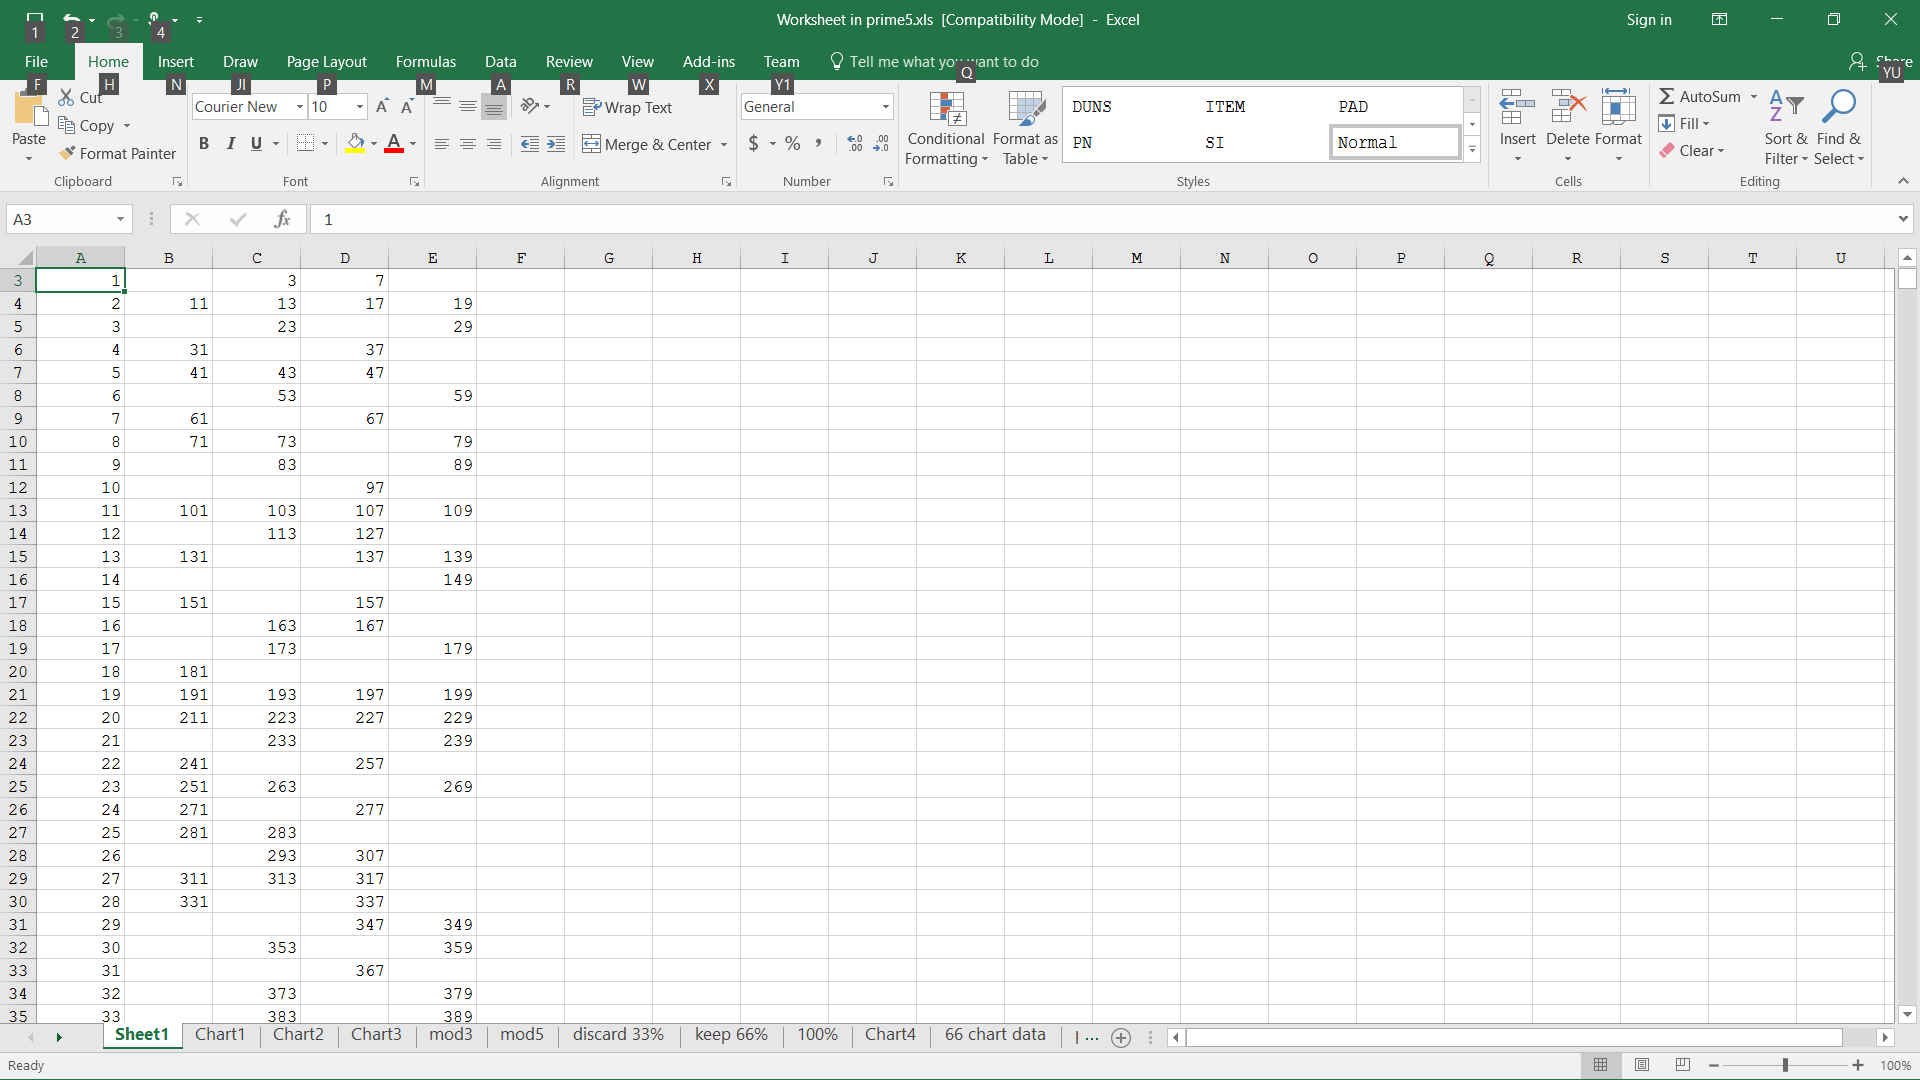
\includegraphics{00b broken line chart data.png}     
\begin{figure}[h]
	\centering
	\includegraphics[width=180mm, height=150mm]{"00b broken line chart data".png}
	\caption{Data for *1 *3 *7 *9 Prime Numbers}
\end{figure}
\pagebreak



\par 
 So , here is the graph. It is a broken line graph. I kind of expected that.
But what intrigued me was the little squiggles in the lines. It looked like a spiral.

%%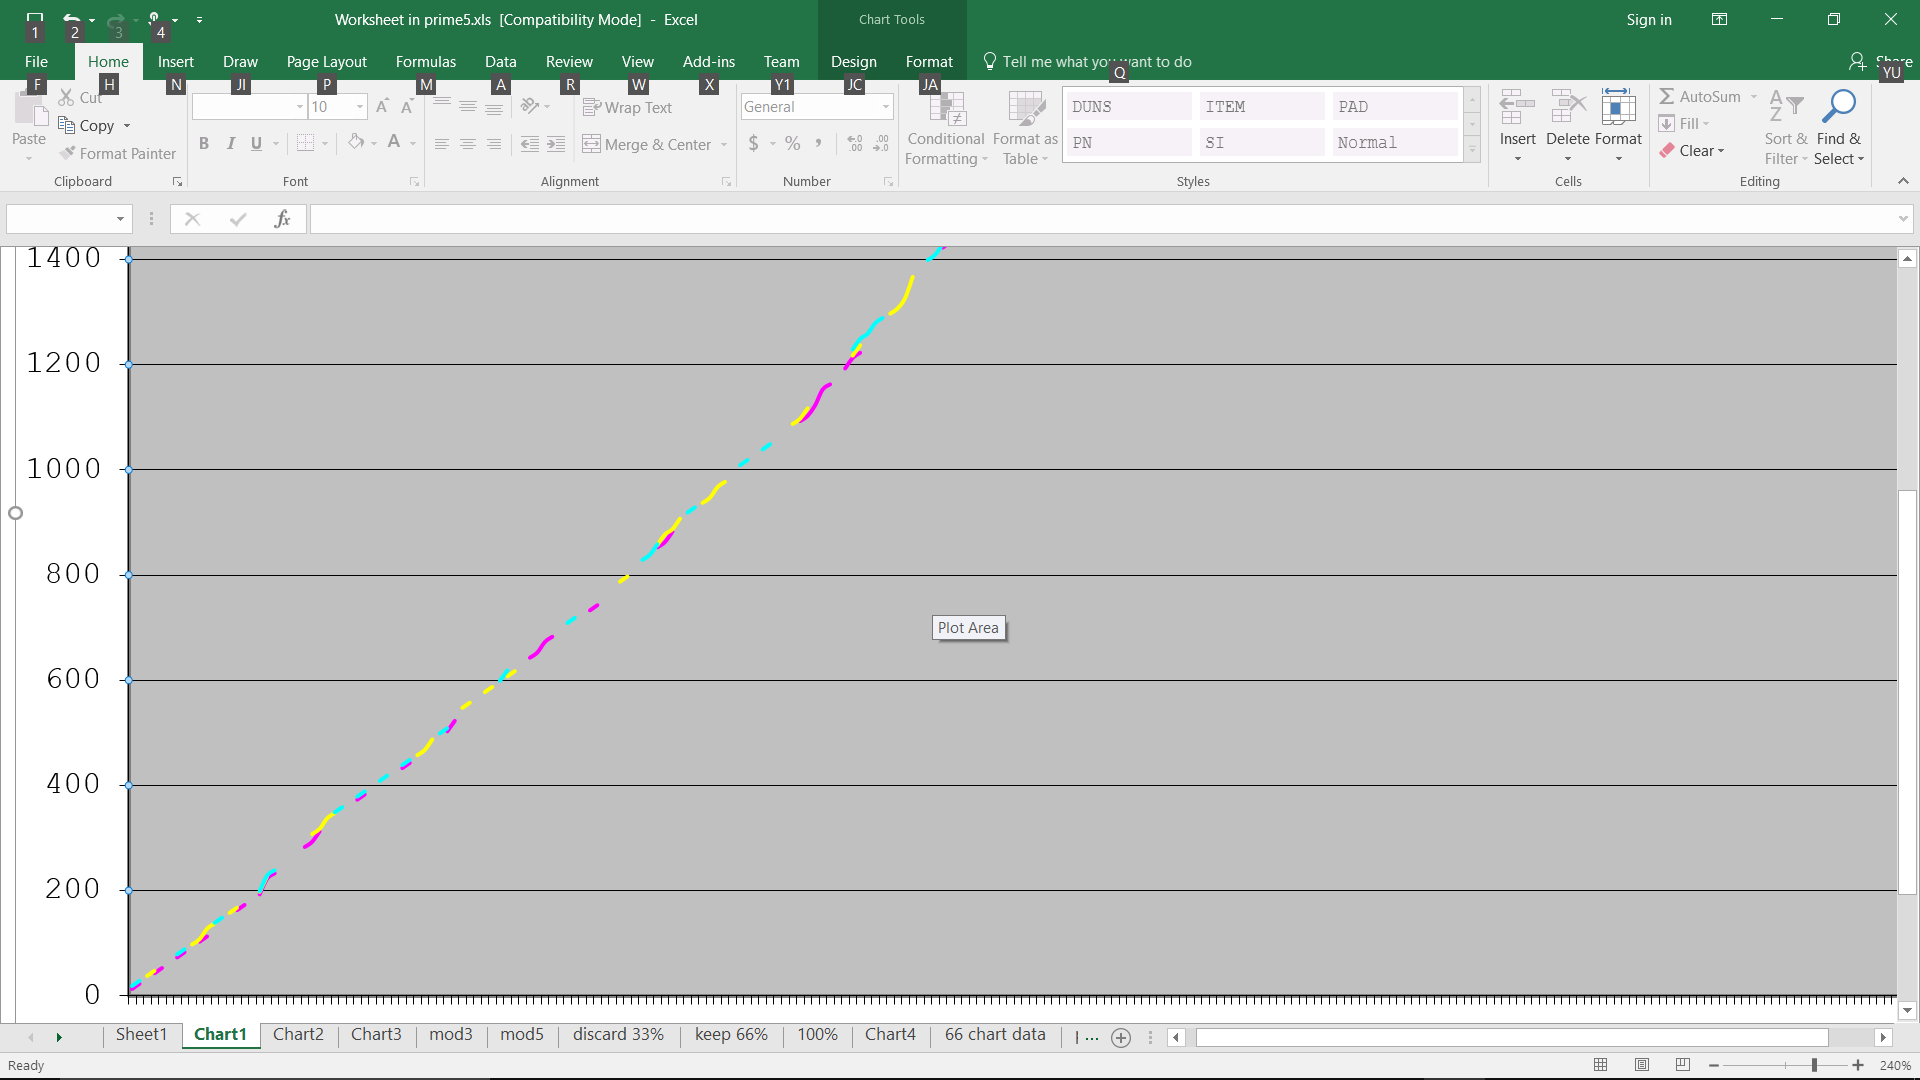
\includegraphics{00a broken line chart.png}  
\begin{figure}[h]
	\centering
	\includegraphics[width=180mm, height=150mm]{"00a broken line chart".png}
	\caption{Squiggle Graph for *1 *3 *7 *9 Prime Numbers}
\end{figure}
\pagebreak   



\section{Scrutinize The Numbers By Inspection}

\par 
The next several charts will show some EXCEL sheets that distill down the view of all numbers to get closer to *wild\textendash card numbers.
\\
\par This chart shows all numbers by the mod function (=MOD (number, divisor)), which will return the remainder of integer division. These cells are conditionally formatted to be yellow if the value is zero (0). This shows were a number can be divided by some other number without a remainder. 
\\
\par Column C is the focus of the division , the painted cells are grouped by color for numbers *1 , *3 , *7 , *9. *Wild\textendash card numbers.
\\
\par Columns D , E , F , . . . are the remainder values. 
\\
\par The gray painted cells relate to the the square root function. Column B is the value of the nearest perfect square. There is a pattern  between the integer number of the perfect square and the remainders  of its neighbors above and below.
%%01 mod all.pn
\begin{figure}[h]
	\centering
	\includegraphics[width=180mm, height=150mm]{"01 mod all".png}
	\caption{Mod All Numbers}
\end{figure}
\pagebreak  


\par 
Lets sort out the even numbers any *2 , *4  , *6 , *8 , *0.
\\
\par 
This will give a closer look at the odd numbers. Same chart just odd numbers only.
\\
\par We are drilling down , we are starting to sort out the unwanted.
%%    02 mod odd.png	
\begin{figure}[h]
	\centering
	\includegraphics[width=180mm, height=150mm]{"02 mod odd".png}
	\caption{Mod Odd Numbers}
\end{figure}
\pagebreak  

\par 
Here is a close up of the prior graphic. 
\\
\par 
Look at 33 , it can be 3 x 11 or 11 x 3
\\
\par 
35 shows 5 x 7 and 7 x 5 , they are situated on both sides of 6. The square root of 36.
\\
\par 
One last look , 49 (circled) is 7 x 7. No matter what.
\\
\par 
We only need to look as far as the square root to determine if a number is prime.

\begin{figure}[h]
	\centering
	\includegraphics[width=180mm, height=150mm]{"04 mod odd sqrt B".png}
	\caption{Mod Odd Square Root B}
\end{figure}
\pagebreak  

%%%%%%%%%%%%%%%%%%%%%%%%
%%%%%%%%%%%%%%%%%%%%%%%%%
\par 
Right side of square root is redundant.
\\
\par 
Before I get too far ahead of myself , the right side of the square root can be eliminated.
It is just the inverse of the left side. An example is (7 x 11) the same as (11 x 7). They are mirror images on both sides of the square root.
%%"04 mod odd sqrt".png
\begin{figure}[h]
	\centering
	\includegraphics[width=180mm, height=150mm]{"04 mod odd sqrt".png}
	\caption{Mod Odd Square Root}
\end{figure}
\pagebreak


%%%%%%%%%%%%%%%%%%%%%%
%%\subsection[Sort out 5]{title sort}
%% \\
\par 
Lets sort out the *5.
\\
\par 
I still have 2 and 5 , but I will get rid of them soon.
\\
\par 
This will give a larger view of the prior graphic. Here the color coding is getting close.
If you look closely the only yellow cells are in column E and the ending column of the mod function. Yes , I know this is all manual. 
\\
\par 
Here is the start of the primes with color coding by the least significant digit.
%%02 mod odd 2b.png     
\begin{figure}[h]
	\centering
	\includegraphics[width=180mm, height=150mm]{"02 mod odd 2b".png}
	\caption{Mod Odd Numbers B}
\end{figure}
\pagebreak  



\par There are eight separate formulas that can color code the numbers on the prior graphics.
%%"03 formula".png
\begin{figure}[h]
	\centering
	\includegraphics[width=180mm, height=150mm]{"03 formula".png}
	\caption{The Formula by Color}
\end{figure}
\pagebreak  

\section{2 And 5 Are Out}
\par 
At this point lets look at 2 (two) and 5 (five).
\\
\par 
Both of these number are each a one shot , they only occur once 
as the least significant digit.
\\
It is extraneous data , sort them out.
\\
\subsection{2 - Deuces Are Wild}
\par 
Two (2) is the only even number prime number. 
All subsequent even numbers are just a multiple of two (2). 
There will never be any number that is *2 greater than 2 that can be prime.
\\
\\
\begin{center}
\begin{tabular}{|c|c|c|c|c|c|c|c|c|c|}
	\hline 
	1 & 2 & 3 & 4 & 5 & 6 & 7 & 8 & 9 & 10 \\ 
	\hline 
	2 & 4 & 6 & 8 &10  &12  &14  &16  &18 & 20 \\ 
	\hline 
\end{tabular} 
\end{center}
\vspace*{2mm}
\captionof{figure}{Deuces.}
\vspace*{4mm}


\par 
The top row is the start of integer values. The bottom row is the result of multiplication by two (2)  ; all even digits.
All divisible by two (2).
%%%%%%%%%%%%
\subsection{5 - Five Is Alone}
\par 
Five (5) is just like two (2) there is only one prime that will end with a five. All the rest are multiples of five (5). There will never be any number that is *5 greater than five (5) that can be prime.
\\
\\
\begin{center}
    \begin{tabular}{|c|c|c|c|c|c|c|c|c|c|}
       	\hline 
       1 & 2 & 3 & 4 & 5 & 6 & 7 & 8 & 9 & 10 \\ 
       \hline 
       5 & 10 & 15 & 20 & 25  &30  &35  &40  &45 & 50 \\ 
       \hline 
    \end{tabular} 
\end{center}
\vspace*{2mm}
\captionof{figure}{Fives.}
\vspace*{4mm}

\par 
The top row is the start of integer values. The bottom row is the result of multiplication by the top row. Any even* number time five (5) will give a *0 number. Any *odd number times five (5) will give a *5 number. 
\\
\\
Remember *wild\textendash card numbers.
\pagebreak




\section{How And Why Can We Discard Numbers}
\par 
In the real world we make all kinds of different sorts  for different data ; different  rules  ; for all kinds of different situations. 
\\
\par 
The first that comes to mind is the old MS-DOS ``dir'' command.
\\
 We could sort files with ``dir a*.com'' - give me a list of all files that starts with ``a'' , and are any length or values and have a ``com'' extension.
\\
\par 
Next ,  in a TSO Mainframe File Edit , is a command like `` sort 12 15 a 23 34 d 16 18 a '' - sort columns 12 to 15 ascending , and then 23 to 34 descending , and finally 16 to 18 ascending.
\\
\par 
In another program we could say:
\\
`` define pick/a1 = if ((stkm = edit(******9) = `r') or (stkm = edit(*****9*) = `r')) then `Y' else ` ' ;  ''
\\ 
if pick equals ``Y'' (yes) then later select (sort in) these records. Do not select (sort out) the blank `` '' records.
\\
\par 
Finally , my favorite and hopefully best argument.
\\
\par 
In any good text editor is a thing called regex (regular expression). It allows for pattern matching in a file.
 I won't go to deep here ; but this is a perfect example of the text \textbf{\underline{(read: data)}}  tool being developed for the need.
\\
\par 
In my text editor KEDIT an example would be: `` locate reg /z?c/ ''. Locate any string that starts with a ``z'' and has ``any character'' and ends with a ``c''.
\\
\par
Google `` regular expression '' for real fun! Read the history.
\\
\par 
All of the above examples are really a sort ; sorting out what we don't want and sorting in what we want to keep. Each is a different tool based on the data.
\\
\par



\pagebreak 
%%%%%%%%%%%%D
\section{Let Us Go Hunt For The Sort And Formula(s)}
\par 
In the below slide are \underline{\textbf{all}} the possible integers sorted by their least significant digit. 
\\
\par
Once again remember *wild\textendash card numbers.
\\
\par 
There are ten piles of numbers.  From *0 , *1 , *2 ,  . . . , *9.
\\
\par
Yellow colored are even numbers , and green colored are odd numbers.
\\
%%"50 wild-card".png
\begin{figure}[h]
	\centering
	\includegraphics[width=180mm, height=150mm]{"50 wildcard".png}
	\caption{Color Code Yellow = Even And Green = Odd }
\end{figure}

\pagebreak  


\par 
Next , let's sort the even (yellow) to the left ; and odd (green) to the right.
%%"52 wildcard".png
\begin{figure}[h]
	\centering
	\includegraphics[width=180mm, height=150mm]{"52 wildcard".png}
	\caption{Even Odd Sort By Color}
\end{figure}

\pagebreak

\par 
Next move the *5 next to the yellow and in front of the *1. This is an sort based on eliminating the *5 from above.
%%"54 wildcard".png
\begin{figure}[h]
\centering
\includegraphics[width=180mm, height=150mm]{"54 wildcard".png}
\caption{Move *5}
\end{figure}
\pagebreak

\par 
The color of *5 in now yellow , we have discarded it.
\par
This leaves the numbers *1 and *3 and *7 and *9 for the hunt.
%%"56 wildcard".png
\begin{figure}[h]
\centering
\includegraphics[width=180mm, height=150mm]{"56 wildcard".png}
\caption{Change *5 to Yellow}
\end{figure}
\pagebreak

\par 
What is unique about these numbers is the location to nearby 5 (five) and zero (0).
\\
\par 
It appears that all prime numbers hover around *5 and *0.
\\
\par 
So , 
\\
\par
\begin{tabular}{rrrr}
%	\hline 
	\rule[-1ex]{0pt}{2.5ex}  \hspace{1cm}&*1&is&*0 + 1\\ 
%	\hline 
	\rule[-1ex]{0pt}{2.5ex}  \hspace{1cm}&*3&is& *5 - 2\\ 
%	\hline 
	\rule[-1ex]{0pt}{2.5ex}  \hspace{1cm}&*7&is&*5 + 2\\ 
%	\hline 
	\rule[-1ex]{0pt}{2.5ex}  \hspace{1cm}&*9&is& *0 - 1\\ 
%	\hline 
\end{tabular} 
%%"58 wildcard 5+-2 or 0+-1".png
\begin{figure}[h]
\centering
\includegraphics[width=180mm, height=150mm]{"58 wildcard 5+-2 or 0+-1".png}
\caption{*5 +/- 2 or *0 +/- 1}
\end{figure}
\pagebreak

\par
We can further sort out one-third (1/3) of the remaining numbers. Every third occurrence will be a multiple of three (3).
I promise to get you to the end. Trust me  . . .
\\
%%"60 wildcard 5+-2 or 0+-1 3rd".png
\begin{figure}[h]
\centering
\includegraphics[width=180mm, height=150mm]{"60 wildcard 5+-2 or 0+-1 3rd".png}
\caption{Eliminate One-Third of *1 , *3 , *7 , *9}
\end{figure}
\pagebreak


\par 
So we are left with a patch of numbers to look at.
\\
\par
 Some serious number theorist will disagree but we have eliminated a percentage of numbers. 
\\
\par 50\% for the *even numbers , 10 \% for the *5 numbers. Then 33\% of each of the rest. 
\\
\par 
So 33\% of 10\% for four occurrences. .333 x .10 x 4 = .1332 or $\approx$ 13.32\%
\\
\par 
Added all up is $\approx$ 73.32\% are gone. We have to look at the balance , $\approx$ 26.68\% of the numbers.
\\	
\par 
Take 8 $\div$ 30 = $\approx$ 26.68\%
%%"62 wildcard 5+-2 or 0+-1 3rd".png
\begin{figure}[h]
\centering
\includegraphics[width=180mm, height=150mm]{"62 wildcard 5+-2 or 0+-1 3rd".png}
\caption{\% Of What Is Left}
\end{figure}
\pagebreak




%%"64 wildcard 5+-2 or 0+-1 3rd".png
\begin{figure}[h]
\centering
\includegraphics[width=180mm, height=150mm]{"64 wildcard 5+-2 or 0+-1 3rd".png}
\caption{Just Another View Of The World}
\end{figure}
\pagebreak


\par 
Let's zoom in on *3. 
\\
\par 
Just to be clear from here on out when you see and read (3)(10) think the first four primes (1)(2)(3)(5) . 
\par  
So , 1 x 2 x 3 x 5 (1 times 2 times 3 times 5). 
\\
\par 
The graphics shows the formulas stacked three high , and for the results for n = 0 , 1 , 2 , 3 and 4.
\\ 
\\
\hspace*{6mm}
\colorbox{yellow}{\textbf{ 3 + n(3)(10) }} 
\hspace*{12mm}
\colorbox{green}{\color{cyan}{\textbf{ 13 + n(3)(10) }}}  
\hspace*{12mm}
\colorbox{green}{\color{cyan}{\textbf{ 23 + n(3)(10) }}} 
%\begin{tabular}{|r|r|r|}
%\hline
%\colorbox{yellow}{\textbf{ 3 + n(3)(10) }} 
%& \colorbox{green}{\color{white}{\textbf{ 13 + n(3)(10) }}}  
%& \colorbox{green}{\color{orange}{\textbf{ 23 + n(3)(10) }}} 
%\\ 
%\hline
%\end{tabular} 
\\
\par 
The yellow cells are divisible by three (3). These are the one-third that we can eliminate.
The green cells are the focus of our search. 
\\	
\par 
These formulas will give all *3 numbers for n = 0 , 1 , 2 , 3 , . . . , $\infty$ . 	
\\

%%"66 wildcard forumla 01 for 3".png
\begin{figure}[h]
\centering
\includegraphics[width=180mm, height=150mm]{"66 wildcard forumla 01 for 3".pdf}
\caption{Zoom In On *3}
\end{figure}
\pagebreak
	


%%%%%%%%%%%%%%%%%%%%%%%
\par 
Just for clarification.
%%"68 wildcard forumla 02 for 3".png
\begin{figure}[h]
	\centering
	\includegraphics[width=180mm, height=150mm]{"68 wildcard forumla 02 for 3".pdf}
	\caption{Zoom In On *3 Formulas Only}
\end{figure}
\pagebreak


\par 
Here is another view of the *3 formulas and the results.
%%"70 wildcard forumla 03 for 3".png
\begin{figure}[h]
	\centering
	\includegraphics[width=180mm, height=150mm]{"70 wildcard forumla 03 for 3".pdf}
	\caption{Zoom In On *3 Formula Results Only}
\end{figure}
\pagebreak




\par 
Here are the *1 , * 3 , *7 , *9 numbers with the one-third number color coded yellow to eliminate the division by 3 portion.
\\ 
\par 
This same argument can be carried from *3 to the other numbers.
%%"72 wildcard formula to remove 3rds graph 02".png
\begin{figure}[h]
	\centering
	\includegraphics[width=180mm, height=150mm]{"72 wildcard formula to remove 3rds graph 02".png}
	\caption{0 +/- 1 and 5 +/-2 With Color}
\end{figure}
\pagebreak



\par 
Here are all the numbers from one (1) to thirty (30) with color coding for division by three (3).
%%"72 wildcard formula to show matrix all numbers".png
\begin{figure}[h]
	\centering
	\includegraphics[width=180mm, height=150mm]{"72 wildcard formula to show matrix all numbers".png}
	\caption{All Numbers By Color}
\end{figure}
\pagebreak


\par 
The next graphic is a matrix of formulas with an input of a value for n. And , the results.
\\
\par 
The top line is *1 , *3 , *7 , *9  or  0 + 1 , 5 - 2 , 5 + 2 , 0 - 1. 
The next three lines in the box are the formulas , every three lines below have the corresponding formulas.
The yellow painted cell are the ones that can be divided by three (3). The `n' heading in row 4 is the input value to the formulas. 
\\
\par 
It is funny , but note the numbers are all ten (10) apart. If you eliminate the yellow divisible by three (3) then it would appear that prime numbers \textbf{could} be ten (10) apart , followed by a gap of twenty (20)  apart for each column.
\\
\par 
So what do we have? A set of formulas that will list the possible prime numbers.

%%"80 100% of 1 3 7 9".png
\begin{figure}[h]
	\centering
	\includegraphics[width=180mm, height=150mm]{"80 100percent of 1 3 7 9".png}
	\caption{Show All Formulas And Results}
\end{figure}
\pagebreak

	
	

\par 
So , here are the formulas that can be sorted off and discarded.  No matter what value of `n' ; these are all divisible by three (3). I am going to allow the number three (3) be discarded at this time. I am just going to let it slip away.
%%"82 33% discard of 1 3 7 9".png
\begin{figure}[h]
	\centering
	\includegraphics[width=180mm, height=150mm]{"82 33percent discard of 1 3 7 9".png}
	\caption{Discard The One-third}
\end{figure}
\pagebreak


\par 
What is left are the unpainted cells. These are the keepers. Two-thirds of the *1 , *3 , *7 , *9 numbers. 
\\	
%%"84 66% keep of 1 3 7 9".png
\begin{figure}[h]
	\centering
	\includegraphics[width=180mm, height=150mm]{"84 66percent keep of 1 3 7 9".png}
	\caption{Keep The Two-thirds}
\end{figure}
\pagebreak


\par 
Now , here is a matrix of formulas that will give all numbers for `n' from 0 , 1 , 2 , 3 , . . . , $\infty$ . 
\\
\par 
The yellow painted cells are now the guys we want to take a closer look at.				
%%"86 just 1 3 7 9 formulas".png
\begin{figure}[h]
	\centering
	\includegraphics[width=180mm, height=150mm]{"86 just 1 3 7 9 formulas 2".png}
	\caption{Matrix of Formulas}
\end{figure}
\pagebreak
			
	
\par 
Here is the formula matrix. The ``initial matrix''  is from 1 to 30 as a constant.
\\
\par 
The ``Actual formulas in E , F , G'' matrix is the definition of the formulas in the respective columns.
\\
\par 
The input value is in cell E3. Just below `n'.
\\
\par 
The ``formulas for above result matrix'' is the human readable formula (a constant (1 to 30)) plus the quantity of a variable `n' times (1*2*3*5)).
The ``result matrix'' will yield all numbers from zero (0) to infinity ($\infty$) .
\\ 
\par 
In this example n = 5.
%%"88 all odd and even formulas".png
\begin{figure}[h]
	\centering
	\includegraphics[width=180mm, height=150mm]{"88 all odd and even formulas".png}
	\caption{Formula Matrix}
\end{figure}
\pagebreak


\par 
The formula will also work for negative numbers of `n'. Here n = \textendash 1.
\\
\par 
So , the formulas are valid for numbers:
\\
\par 
 \textendash\space  $\infty$ , . . . , -3 , -2 , -1 , 0 , 1 , 2 , 3 , . . .  , + $\infty$
%%"88 negitive".png
\begin{figure}[h]
	\centering
	\includegraphics[width=180mm, height=150mm]{"88 negative".png}
	\caption{Formula Matrix With \textendash 1}
\end{figure}
\pagebreak


			
\par 
This graphic shows values of `n'  equal to 0 , 1 , 2 , 3 , 4 , 5. The results are from 1 to 180.

%%"90 all odd and even results 0-5".png
\begin{figure}[h]
	\centering
	\includegraphics[width=180mm, height=150mm]{"90 all odd and even results 0-5".png}
	\caption{Results For n = 0 to 5}
\end{figure}
\pagebreak[4]
\clearpage


\par 
Here are the formulas that have \textbf{not} been sorted out with their color coding.
%%"92 1 3 7 9 formula".png
\begin{figure}[h]
	\centering
	\includegraphics[width=180mm, height=150mm]{"92 1 3 7 9 formula".png}
	\caption{Sorted In Formulas by Color}
\end{figure}
\pagebreak[4]
\subsection{Cash Constant 00}
*wild\textendash card numbers - there is a set of numbers listed by the least significant digit.
\clearpage 
\pagebreak[4]
\subsection{Cash Constant 01}
*1 *3 *7 *9 - after sorting off unwanted numbers , these are of interest to find primes from seven (7) and higher.
\clearpage 
\pagebreak[4]
\subsection{Cash Constant 02}
*fam equations - after sorting again to remove numbers divisible by three (3). There are eight (8) equations to look for and attempt to solve for primes.
The eight *fam 's are *fam1 , *fam7 , *fam11 , *fam13 , *fam17 , *fam19 , *fam23 , and *fam29. These are subfamilies of *wild\textendash card numbers.


\clearpage
\pagebreak[4]
\section{The Cash Pile}
\subsection{Matrix}
\par 
Here is the full matrix with the possible primes painted in yellow. We have eliminated any 
\\
 *even , * (divisible by 3) , and *5.
\\
\\
Our formula has ( 1 x 2 x 3 x 5) the first four (4) primes. So , later when we start looking for prime we can start at seven (7). 
\\
\\
The eight equations will only work for the remaining numbers that we want to search through. 
\\
%%%%%   LEARN     %%%%%%%%%%%%%%%%%%%%%
%%%%%%%%%%%%%%%%%%%%%%%%%%%%%%%%

\begin{tikzpicture}[every node/.style={anchor=north east ,fill=white,minimum width=3cm,minimum height=15mm}]

\matrix (mA) [draw,matrix of math nodes]
{
	\colorbox{yellow}{ =1 + (n)(3)(10)}   &   \colorbox{yellow}{= 11 + (n)(3)(10) }   &     =21 + (n)(3)(10)   &    \\
	=2 + (n)(3)(10)   &   =12 + (n)(3)(10)    &     =22 + (n)(3)(10)   &    \\
	=3 + (n)(3)(10)   &   \colorbox{yellow}{ =13 + (n)(3)(10) }   &   	\colorbox{yellow}{ =23 + (n)(3)(10) }  &    \\
	=4 + (n)(3)(10)   &   =14 + (n)(3)(10)    &     =24 + (n)(3)(10)   &    \\
	=5 + (n)(3)(10)   &   =15 + (n)(3)(10)    &     =25 + (n)(3)(10)   &    \\
	=6 + (n)(3)(10)   &   =16 + (n)(3)(10)    &     =26 + (n)(3)(10)   &    \\
	\colorbox{yellow}{ =7 + (n)(3)(10) }   &   \colorbox{yellow}{ =17 + (n)(3)(10) }    &     =27 + (n)(3)(10)   &    \\
	=8 + (n)(3)(10)   &   =18 + (n)(3)(10)    &     =28 + (n)(3)(10)   &    \\
	=9 + (n)(3)(10)   &   \colorbox{yellow}{ =19 + (n)(3)(10) }    &     \colorbox{yellow}{ =29 + (n)(3)(10) }   &    \\
	=10 + (n)(3)(10)  &   =20 + (n)(3)(10)   &     =30 + (n)(3)(10)    &  
	\colorbox{green}{n = \textendash $\infty$ , . . . ,  + $\infty$} \\
};



%\pagebreak

\end{tikzpicture}
\captionof{figure}{Cash Pile Formulas.}
\pagebreak




%%%%%%%%%%%%%%%%%%%%%%%%%%%%%%%%%%
\subsection{Results}
\par 
Here are the results matrix with the possible primes painted in yellow. 
\\
This is for values of `n' =  -1 , 0 , 1 , 2.  The lowest number is in the top left corner , and the highest is in the bottom right corner.	
%\\
%This is for values of `n' =  -1 , 0 , 1 , 2.  The lowest number is in the top left corner , and the highest is in the bottom right corner.	
\\
\begin{center}

\begin{tikzpicture}[every node/.style={anchor=north east ,fill=white,minimum width=1cm,minimum height=5mm}]
\tiny
\matrix (mA) [draw,matrix of math nodes]
{
    \colorbox{yellow}{(61)}   &                   (66)    &  \colorbox{yellow}{(71)} &                   (76)  &                   (81)   &                    (86)   &  \\
    (62)    & \colorbox{yellow}{(67)}   &                    (72)  & \colorbox{yellow}{(77)} &                   (82)   &                    (87)   &  \\
    (63)    &                   (68)    &  \colorbox{yellow}{(73)} &                   (78)  & \colorbox{yellow}{(83)}  &                    (88)   &  \\
    (64)    &                   (69)    &                    (74)  & \colorbox{yellow}{(79)} &                   (84)   &  \colorbox{yellow}{(89)}  &  \\
    (65)    &                   (70)    &                    (75)  &                   (80)  &                   (85)   &                    (90)   &  \colorbox{green}{\textcolor{red}{\textbf{n = 2}}} \\
};
\matrix (mB) [draw,matrix of math nodes] at ($(mA.south west)+(4,-1)$)
{
    \colorbox{yellow}{(31)}   &                   (36)    & \colorbox{yellow}{(41)} &                   (46)  &                    (51)    &                   (56)    &  \\
    (32)    & \colorbox{yellow}{(37)}   &                   (42)  & \colorbox{yellow}{(47)} &                    (52)    &                   (57)    &  \\
    (33)    &                   (38)    & \colorbox{yellow}{(43)} &                   (48)  &  \colorbox{yellow}{(53)}   &                   (58)    &  \\
    (34)    &                   (39)    &                   (44)  & \colorbox{yellow}{(49)} &                    (54)    & \colorbox{yellow}{(59)}   &  \\
    (35)    &                   (40)    &                   (45)  &                   (50)  &                    (55)    &                   (60)    & \colorbox{green}{\textcolor{red}{\textbf{n = 1}}} \\
};  
\matrix (mC) [draw,matrix of math nodes] at ($(mB.south west)+(4,-1)$)
{
 \colorbox{yellow}{(1)}   &                   (6)   &  \colorbox{yellow}{(11)}  & (16)                    & (21)                     &  (26)                     &  \\
(2)    & \colorbox{yellow}{(7)}  &  (12)                     & \colorbox{yellow}{(17)} & (22)                     &  (27)                     &  \\
(3)    &                   (8)   &  \colorbox{yellow}{(13)}  & (18)                    & \colorbox{yellow}{(23)}  &  (28)                     &  \\
(4)    &                   (9)   &  (14)                     & \colorbox{yellow}{(19)} & (24)                     &  \colorbox{yellow}{(29)}  &  \\
(5)    &                  (10)   &  (15)                     & (20)                    & (25)                     &  (30)                     &  \colorbox{green}{\textcolor{red}{\textbf{n = 0}}} \\
};
\matrix (mD) [draw,matrix of math nodes] at ($(mC.south west)+(4,-1)$)	
{   
    \colorbox{yellow}{(-29)}  &                  (-24)   & \colorbox{yellow}{(-19)} &                   (-14)  &                    (-9)   &                    (-4)   &  \\
    (-28)   &\colorbox{yellow}{(-23)}  &                   (-18)  & \colorbox{yellow}{(-13)} &                    (-8)   &                    (-3)   &  \\
    (-27)   &                  (-22)   & \colorbox{yellow}{(-17)} &                   (-12)  &  \colorbox{yellow}{(-7)}  &                    (-2)   &  \\
    (-26)   &                  (-21)   &                   (-16)  & \colorbox{yellow}{(-11)} &                    (-6)   &  \colorbox{yellow}{(-1)}  &  \\
    (-25)   &                  (-20)   &                   (-15)  &                   (-10)  &                    (-5)   &                     (0)   &  \colorbox{green}{\textcolor{red}{\textbf{n = - 1}}} \\
};                                   



\draw[dashed](mA.north east)--(mD.north east);
\draw[dashed](mA.north west)--(mD.north west);
\draw[dashed](mA.south east)--(mD.south east);
\normalfont 
\end{tikzpicture}
\end{center}

\vspace*{2mm}
\captionof{figure}{Matrix Results Of Cash Pile.}
\vspace*{4mm}


\pagebreak



\subsection{3D View Of The Cash Pile}
\par 
This is a view of the Cash Pile , here is a \textbf{small portion} of the numbers. The bottom face is a 5x6 matrix of the formulas. The right hand face is  `n' with each row the same value. In the interior are the results. This is just a \textbf{pile} of numbers that goes on forever  ; down (\textendash $\infty$ ) or up (+ $\infty$).
\\
\\
\begin{center}

\begin{tikzpicture}
{
    \tikzcuboid{%
        shiftx=4cm,%
        shifty=0cm,%
        scale=0.90,%
        rotation=-83,%
        densityx=1,%
        densityy=1,%
        densityz=2,%
        dimx=10,%
        dimy=5,%
        dimy=5,%
        linefront=red!75!black,%
        linetop=red!50!black,%
        lineright=red!25!black,%
        fillfront=red!25!white,%
        filltop=red!50!white,%
        fillright=red!75!white%
    }
}
\end{tikzpicture}
\end{center}
\vspace*{2mm}
\captionof{figure}{3D View Of The Cash Pile.}
\vspace*{4mm}

\pagebreak
\subsection{Why Is The Pile Important ?}
\par 
\hspace*{6mm} The reverse of finding `n' is important to tell which formula has been matched. An integer value without a decimal remainder shows the intersection of the formula and a level of the Cash Pile. A *3 number can only match one formula.
\\
\par 
There can be a match from both formulas for different numbers on one level , or a missing level match. We will use this later to sort out some *3 data.

%%"92 1 3 7 9 formula".png
\begin{figure}[h]
	\centering
	\includegraphics[width=200mm, height=190mm]{"96 cash pile numbers".pdf}
	\caption{Sorted In Formulas by Color}
\end{figure}
\pagebreak


\subsection{More Cash Pile Calculation}
\par 
Here are several graphics of calculations for the numbers (35679 , 2 , 121 , 19 , 15485863). Each chart shows in the value column which *fam equation has satisfied the equation with an integer value. the ``n'' column shows the height in the Cash Pile. And , the equation column shows what is happening in the ``n'' column. Just a little more proof , that the Cash Pile is solid. 
\\
%%Cash Pile Calc
\begin{figure}[h]
    \centering
    \includegraphics[width=180mm, height=150mm]{"cash Pile Calc 1".pdf}
    \caption{35679}
\end{figure}
\pagebreak


%%Cash Pile Calc
\begin{figure}[h]
    \centering
    \includegraphics[width=180mm, height=150mm]{"cash Pile Calc 2".pdf}
    \caption{2}
\end{figure}
\pagebreak


%%Cash Pile Calc
\begin{figure}[h]
    \centering
    \includegraphics[width=180mm, height=150mm]{"cash Pile Calc 3".pdf}
    \caption{121}
\end{figure}
\pagebreak


%%Cash Pile Calc
\begin{figure}[h]
    \centering
    \includegraphics[width=180mm, height=150mm]{"cash Pile Calc 4".pdf}
    \caption{19}
\end{figure}
\pagebreak


%%Cash Pile Calc
\begin{figure}[h]
    \centering
    \includegraphics[width=180mm, height=150mm]{"cash Pile Calc 5".pdf}
    \caption{15485863}
\end{figure}
\pagebreak     


\subsection{Cash Constant 03}
The first four primes  1 , 2 , 3 , 5 are unique. These are the only consecutive primes that can be added together to make the next prime.
\\
1 + 2 = 3
\\
2 + 3 = 5 
\\
\par 
Next , these four (4) can be multiplied to make the Cash Pile.
\\
1 x 2 x 3 x 5 = 30
\\
\\
I will call these four (4) primes \textbf{``simple primes''} because they start the process. As opposed to complex primes seven (7) and higher. Any primes added together from seven (7) and higher will be an even number. And , any multiplication of odds will just be factors ; and not of one (1) and the number (prime definition).

\clearpage 
\pagebreak[4]
%%%%%%%%%%% %%%%%%%%%%%%%%%%%%%%%
%%%%%%%%%%%%%%%%%%%%%%%%%%%%%%%%
%%%%%%% y = mx + b %%%%%%%%%%%%%%%%%%%
%%%%%%%%%%%%%%%%%%%%%%%%%%%%%%%%%%
%%%% start heredone - show data - add pages - and move up
\section{y = mx + b} 
\par 
This graph is each of the eight formulas in the form of \textbf{y = mx + b}. 
\\Each pair of colors is part of a *wild\textendash card number.
\\
% \colorbox{blue}{\textcolor{yellow}*1} is \colorbox{blue}{blue}
\large
\textbf{\textcolor{blue}{*1 is blue}} \space ; \space \textbf{\textcolor{red}{*3 is red}} 
\\
\textbf{\textcolor{green}{*7 is green}} \space ; \space \textbf{\textcolor{cyan}{*9 is cyan}} 
\\
\normalfont
\\
\begin{tikzpicture}[scale=\textwidth/6cm,]
\begin{axis}[
axis lines = middle,
title={*Wild\textendash Card Lines},
%xlabel={X},
%ylabel={Y},
xmin=-1, xmax=3,
ymin=-30, ymax=120,
xtick={-1,0,1,2,3},
ytick={0,10,20,30,40,50,60,70,80,90,100,110},
legend pos=north west,
ymajorgrids=true,
xmajorgrids=true,
grid style=dashed,
]
%%%%%%  1  %%%%%%%%%%%%
\addplot[
color=blue,
mark=.,
]
coordinates {
	(-1,-29)(0,1)(1,31)(2,61)(3,91)
};
%\legend{CuSO$_4\cdot$5H$_2$O}
%%%%%%  11 %%%%%%%%%%%%%
\addplot[
color=blue,
mark=.,
]
coordinates {
	(-1,-19)(0,11)(1,41)(2,71)(3,101)
};
%%%%%%%  13 %%%%%%%%%%%%
\addplot[
color=red,
mark=.,
]
coordinates {
	(-1,-17)(0,13)(1,43)(2,73)(3,103)
};
%%%%%%%  23  %%%%%%%%%%%%%
\addplot[
color=red,
mark=.,
]
coordinates {
	(-1,-7)(0,23)(1,53)(2,83)(3,113)
};
%%%%%  07  %%%%%%%%%%%%%%
\addplot[
color=green,
mark=.,
]
coordinates {
	(-1,-23)(0,7)(1,37)(2,67)(3,97)
};
%%%%%%  17 %%%%%%%%%%%%%
\addplot[
color=green,
mark=.,
]
coordinates {
		(-1,-13)(0,17)(1,47)(2,77)(3,107)
};

%%%%%%%%    19  %%%%%%%%%%%%%%%
\addplot[
color=cyan,
mark=.,
]
coordinates {
	(-1,-11)(0,19)(1,49)(2,79)(3,109)
};

%%%%%%%%%%%%%%%%%%%%%%%
%%%%%%%%    29  %%%%%%%%%%%%%%%
\addplot[
color=cyan,
mark=.,
]
coordinates {
	(-1,-1)(0,29)(1,59)(2,89)(3,119)
};
%%%%%%%%%%%%%%%%%%%%%%%

\end{axis}
\end{tikzpicture}

\vspace*{2mm}
\captionof{figure}{*Wild-Card Lines.}
\vspace*{4mm}
%%%%%%%%%%%%%%%%%%%%%%%%%%%%%%%%%%%
%%%%%%%%%%%%%%%%%%%%%%%%%%%%%%%%%%%
%%%% close look at y axis
%%%%%%%%%%%%%%%%%%%%%%%%%%%%%%%%%%
%%%%%%%%%%%%%%%%%%%%%%%%%%%%%%%%%%
\pagebreak
\section{Closer Look At Y Axis}
\par 
Closer look at the y axis.
\\
\par 
Each pair of colors is part of a *wild\textendash card number.
\\
% \colorbox{blue}{\textcolor{yellow}*1} is \colorbox{blue}{blue}
\large
\textbf{\textcolor{blue}{*1 is blue}} \space ; \space \textbf{\textcolor{red}{*3 is red}} 
\\
\textbf{\textcolor{green}{*7 is green}} \space ; \space \textbf{\textcolor{cyan}{*9 is cyan}} 
\\
%\textbf{\textcolor{gray}{+ sign is the middle}}
\normalfont
\\
\\
\begin{tikzpicture}[scale=\textwidth/6cm,]
\begin{axis}[
axis lines = middle,
title={Y Axis Close Up},
%xlabel={X},
%ylabel={Y},
xmin=-1, xmax=1,
ymin=-30, ymax=60,	
xtick={-1,0,1},
%ytick={-20,-15,-10,-5,0,5,10,15,20,25,30,35,40,45,50,55,60},
%ytick={1,3,7,9,11,13,17,19,23,29},
legend pos=north west,
ymajorgrids=true,
xmajorgrids=true,
grid style=dashed,
]
%\addplot[
%color=gray,
%mark=+,
%]
%coordinates {
%(-1,-15)(-0.875,-11.25)(-0.75,-7.5)(-0.625,-3.75)(-0.5,0)(-0.375,3.75)(-0.25,7.5)(-0.125,11.25)
%(0,15)(0.125,18.75)(0.25,22.5)(0.375,26.25)(0.5,30)(0.625,33.75)(0.75,37.5)(0.875,41.25)(1,45)
%%	(-1,-15)(-.5,0)(0,15)(.5,30)(1,45)
%};
%\legend{CuSO$_4\cdot$5H$_2$O}
%%%%%%  1  %%%%%%%%%%%%
\addplot[
color=blue,
mark=.,
]
coordinates {
	(-1,-29)(0,1)(1,31)
};
%\legend{CuSO$_4\cdot$5H$_2$O}
%%%%%%  11 %%%%%%%%%%%%%
\addplot[
color=blue,
mark=.,
]
coordinates {
	(-1,-19)(0,11)(1,41)
};
%%%%%%%  13 %%%%%%%%%%%%
\addplot[
color=red,
mark=.,
]
coordinates {
	(-1,-17)(0,13)(1,43)
};
%%%%%%%  23  %%%%%%%%%%%%%
\addplot[
color=red,
mark=.,
]
coordinates {
	(-1,-7)(0,23)(1,53)
};
%%%%%  07  %%%%%%%%%%%%%%
\addplot[
color=green,
mark=.,
]
coordinates {
	(-1,-23)(0,7)(1,37)
};
%%%%%%  17 %%%%%%%%%%%%%
\addplot[
color=green,
mark=.,
]
coordinates {
	(-1,-13)(0,17)(1,47)
};
%%%%%%%%    19  %%%%%%%%%%%%%%%
\addplot[
color=cyan,
mark=.,
]
coordinates {
	(-1,-11)(0,19)(1,49)
};
%%%%%%%%%%%%%%%%%%%%%%%
%%%%%%%%    29  %%%%%%%%%%%%%%%
\addplot[
color=cyan,
mark=.,
]
coordinates {
	(-1,-1)(0,29)(1,59)
};
%%%%%%%%%%%%%%%%%%%%%%%
\end{axis}
\end{tikzpicture} 

\vspace*{2mm}
\captionof{figure}{*Wild\textendash Card Lines Close Up.}
\vspace*{4mm}
%%%%%%%%%%%%%%%%%%%%%%%%%%%%%%%%%%%%%%
%%%%%%%%%%%%%%%%%%%%%%%%%%%%%%%%%%%%%%%
\pagebreak
\section{Closer Look At Y Axis For Cash Pile}
\par 
Closer look at the y axis for all thirty (30) equations.
\\
\par 
Each pair of colors is part of a *wild\textendash card number. Just to make sure , here are the rest of the formulas that have been discarded from the Cash Pile. The focus will turn to colored lines only. The data follows on the next page.
\\
% \colorbox{blue}{\textcolor{yellow}*1} is \colorbox{blue}{blue}
\large
\textbf{\textcolor{blue}{*1 is blue}} \space ; \space \textbf{\textcolor{red}{*3 is red}} 
\\
\textbf{\textcolor{green}{*7 is green}} \space ; \space \textbf{\textcolor{cyan}{*9 is cyan}} 
\\
\textbf{\textcolor{black}{black}} are the rest. 
\normalfont
\\
\\
%%%%%%%%%%%%%%%%%%%%%%%%%%%%%%%%%%%%%%%
%%%%%%%%%%%%%%%%%%%%%%%%%%%%%%%%%%%%%%%
%\pagebreak
%\begin{landscape}
    \begin{tikzpicture}[scale=\textwidth/6cm,]
    \begin{axis}[
    axis lines = middle,
    %title={Wild\textendash card Lines},
    %xlabel={X},
    %ylabel={Y},
    xmin=-1, xmax=1,
    ymin=-30, ymax=30,
    xtick={-1,0,1},
    ytick={-30,-20,-10,0,10,20,30},
    legend pos=north west,
    ymajorgrids=true,
    xmajorgrids=true,
    grid style=dashed,
    ]
    %\addplot[
    %color=gray,
    %mark=+,
    %]
    %coordinates {
    %(-1,-15)(-0.875,-11.25)(-0.75,-7.5)(-0.625,-3.75)(-0.5,0)(-0.375,3.75)(-0.25,7.5)(-0.125,11.25)
    %(0,15)(0.125,18.75)(0.25,22.5)(0.375,26.25)(0.5,30)(0.625,33.75)(0.75,37.5)(0.875,41.25)(1,45)
    %%	(-1,-15)(-.5,0)(0,15)(.5,30)(1,45)
    %};
    %\legend{CuSO$_4\cdot$5H$_2$O}
    %%%%%%  1  %%%%%%%%%%%%
    \addplot[color=blue,mark=.,]coordinates {(-1,-29)(0,1)(1,31)};
    %\legend{CuSO$_4\cdot$5H$_2$O}
    %%%%%%  11 %%%%%%%%%%%%%
    \addplot[color=blue,mark=.,]coordinates {(-1,-19)(0,11)(1,41)};
    %%%%%%%  13 %%%%%%%%%%%%
    \addplot[color=red,mark=.,]coordinates {(-1,-17)(0,13)(1,43)};
    %%%%%%%  23  %%%%%%%%%%%%%
    \addplot[color=red,mark=.,]coordinates {(-1,-7)(0,23)(1,53)};
    %%%%%  07  %%%%%%%%%%%%%%
    \addplot[color=green,mark=.,]coordinates {(-1,-23)(0,7)(1,37)};
    %%%%%%  17 %%%%%%%%%%%%%
    \addplot[color=green,mark=.,]coordinates {(-1,-13)(0,17)(1,47)};
    %%%%%%%%    19  %%%%%%%%%%%%%%%
    \addplot[color=cyan,mark=.,]coordinates {(-1,-11)(0,19)(1,49)};
    %%%%%%%%%%%%%%%%%%%%%%
    %%%%%%%    29  %%%%%%%%%%%%%%%
    \addplot[color=cyan,mark=.,]coordinates {(-1,-1)(0,29)(1,59)};
    
    %%%%% the rest %%%%%%%%%%%%%
    %%%%%%%%%%%%%%%%%%%%%%%
    \addplot[color=black,mark=.,]coordinates  { (-1,-29)(0,1)(1,31)                 };   
    \addplot[color=black,mark=.,]coordinates  { (-1,-28)(0,2)(1,32)                 };   
    \addplot[color=black,mark=.,]coordinates  { (-1,-27)(0,3)(1,33)                 };   
    \addplot[color=black,mark=.,]coordinates  { (-1,-26)(0,4)(1,34)                 };   
    \addplot[color=black,mark=.,]coordinates  { (-1,-25)(0,5)(1,35)                 };   
    \addplot[color=black,mark=.,]coordinates  { (-1,-24)(0,6)(1,36)                 };   
    \addplot[color=black,mark=.,]coordinates  { (-1,-22)(0,8)(1,38)                 };   
    \addplot[color=black,mark=.,]coordinates  { (-1,-21)(0,9)(1,39)                 };   
    \addplot[color=black,mark=.,]coordinates  { (-1,-20)(0,10)(1,40)                };   
    \addplot[color=black,mark=.,]coordinates  { (-1,-18)(0,12)(1,42)                };   
    \addplot[color=black,mark=.,]coordinates  { (-1,-16)(0,14)(1,44)                };   
    \addplot[color=black,mark=.,]coordinates  { (-1,-15)(0,15)(1,45)                };   
    \addplot[color=black,mark=.,]coordinates  { (-1,-14)(0,16)(1,46)                };   
    \addplot[color=black,mark=.,]coordinates  { (-1,-12)(0,18)(1,48)                };   
    \addplot[color=black,mark=.,]coordinates  { (-1,-10)(0,20)(1,50)                };   
    \addplot[color=black,mark=.,]coordinates  { (-1,-9)(0,21)(1,51)                 };   
    \addplot[color=black,mark=.,]coordinates  { (-1,-8)(0,22)(1,52)                 };   
    \addplot[color=black,mark=.,]coordinates  { (-1,-6)(0,24)(1,54)                 };   
    \addplot[color=black,mark=.,]coordinates  { (-1,-5)(0,25)(1,55)                 };   
    \addplot[color=black,mark=.,]coordinates  { (-1,-4)(0,26)(1,56)                 };   
    \addplot[color=black,mark=.,]coordinates  { (-1,-3)(0,27)(1,57)                 };   
    \addplot[color=black,mark=.,]coordinates  { (-1,-2)(0,28)(1,58)                 };   
    \addplot[color=black,mark=.,]coordinates  { (-1,0)(0,30)(1,60)                  };   
    %%%%%%%%%%%%%%%%%%%%%%%
    \end{axis}
    \end{tikzpicture} 
%\end{landscape}

\vspace*{2mm}
\captionof{figure}{*Wild\textendash Card All Lines Close Up.}
\vspace*{4mm}
\pagebreak

\par 
This is the data for all the lines in the Cash Pile. So ,  just to keep it honest , here are all thirty (30) equations. The three colored columns are repeats , but have different input values. So ,  y = value column + (input x 30). Look at the blue one (1) column. So , y = 1 + (1 x 30) ; y = 31. Gives us the point (1,31) in column (x3 , y3).
\\
\\ 
This is the data for the plot of x =  -1 , 0 , 1 in the prior graph.
\begin{figure}[h]
    \centering
    \includegraphics[width=180mm, height=150mm]{"Closer Look At Y Axis For Cash Pile Data".pdf}
    \caption{Cash Pile Data}
\end{figure}
\pagebreak



\pagebreak
%%%%%%%%%%%%%%%%%%%%%%%%%%%%%%%%%%%%%%
%%%%%%%%%%%%%%%%%%%%%%%%%%%%%%%%%%%%%%
%%%%%%%%%%%%%%%%%%%%%%%%%%%%%%%%%%%%%%
%%%%%%%%%%%    *3 and square root  %%%%%%%%%%%%%%%
%%%%%%%%%%%%%%%%%%%%%%%%%%%%%%%%%%%%%%
%%%%%%%%%%%%%%%%%%%%%%%%%%%%%%%%%%%%%%
%%%%%%%%%%%%%%%%%%%%%%%%%%%%%%%%%%%%%%
\pagebreak 
\section{*3 Graph And Data}
\subsection{*3 (13) And Square Root And 7} 
\par 
This graph is of a *3 *wild\textendash card number. On the next page is the data.
\\
\large
\textbf{\textcolor{blue}{13 + n(1x2x3x5)}} 
\\
\\
\normalfont
\\
\begin{tikzpicture}[scale=\textwidth/8cm,]
\begin{axis}[
%axis lines = middle,
title={ *3 (13) *Wild\textendash card Lines},
%xlabel={X},
%ylabel={Y},
%xmin=0, xmax=3,
%ymin=-30, ymax=120,
%xtick={-1,0,1,2,3},
%ytick={0,10,20,30,40,50,60,70,80,90,100,110},
legend pos=north west,
ymajorgrids=true,
xmajorgrids=true,
grid style=dashed,
]
%%%%%%%  1  %%%%%%%%%%%%
%\addplot[
%color=blue,
%mark=.,
%]
%coordinates {
%	(-1,-29)(0,1)(1,31)(2,61)(3,91)
%};
%%\legend{CuSO$_4\cdot$5H$_2$O}
%%%%%%%  11 %%%%%%%%%%%%%
%\addplot[
%color=blue,
%mark=.,
%]
%coordinates {
%	(-1,-19)(0,11)(1,41)(2,71)(3,101)
%};
%%%%%%%  13 %%%%%%%%%%%%
\addplot[
color=red,
mark=.,
]
coordinates {
(0,13)(1,43)(2,73)(3,103)(4,133)(5,163)(6,193)
(7,223)(8,253)(9,283)(10,313)(11,343)(12,373)(13,403)(14,433)(15,463)
(16,493)(17,523)(18,553)(19,583)(20,613)(21,643)
};
%%%%%%%  Sq root  %%%%%%%%%%%%%
\addplot[
color=green,
mark=.,
]
coordinates {
(0,3.6055)(1,6.5574)(2,8.5440)(3,10.148)(4,11.532)(5,12.767)(6,13.892)
(7,14.933)(8,15.905)(9,16.822)(10,17.691)(11,18.520)(12,19.313)(13,20.074)(14,20.808)(15,21.517)
(16,22.203)(17,22.869)(18,23.515)(19,24.145)(20,24.758)(21,25.357)
};
%%%%%%%  7 %%%%%%%%%%%%%
\addplot[
color=blue,
mark=.,
]
coordinates {
(0,7)(1,7)(2,7)(3,7)(4,7)(5,7)(6,7)(7,7)(8,7)(9,7)(10,7)(11,7)(12,7)(13,7)(14,7)(15,7)(16,7)(17,7)(18,7)(19,7)(20,7)(21,7)
%%(7,0)(7,1)(7,2)(7,3)(7,4)(7,5)(7,6)(7,7)(7,8)(7,9)(7,10)(7,11)(7,12)(7,13)(7,14)(7,15)(7,16)(7,17)(7,18)(7,19)(7,20)(7,21)
%%%%%%%  Sq root  %%%%%%%%%%%%%
};
\end{axis}
\end{tikzpicture}

\vspace*{2mm}
\captionof{figure}{*fam13 and Square Root and Seven.}
\vspace*{4mm}

\pagebreak 
\subsection{*3 (13 Data)}

\par
The column (x1,y1) is the plot of the red line. The column (x2,y2) is the plot of the green line. This is the square root of the red line (13 + n(3)(10)). The blue line is y = 7. We only need to test the numbers inclusively from blue to green to test red for a non-prime number. Why ? Because any numbers on the other side of the squire root function are just a mirror image of the values less than the square root. Again (7x11) = (11x7) ; just mirror image.
\\
\\
\begin{center}

\begin{tabular}{|r|r|r|r|r|}

\hline   n     & 13+n(3)(10)  &  (x1,y1)      &   sq root13  &  (x2,y2)      \\
\hline   0     & 13           &  (0,13)       &   3.6056     &  (0,3.6055)   \\
\hline   1     & 43           &  (1,43)       &   6.5574     &  (1,6.5574)   \\
\hline   2     & 73           &  (2,73)       &   8.5440     &  (2,8.5440)   \\
\hline   3     & 103          &  (3,103)      &   10.1489    &  (3,10.148)   \\
\hline   4     & 133          &  (4,133)      &   11.5326    &  (4,11.532)   \\
\hline   5     & 163          &  (5,163)      &   12.7671    &  (5,12.767)   \\
\hline   6     & 193          &  (6,193)      &   13.8924    &  (6,13.892)   \\
\hline   7     & 223          &  (7,223)      &   14.9332    &  (7,14.933)   \\
\hline   8     & 253          &  (8,253)      &   15.9060    &  (8,15.905)   \\
\hline   9     & 283          &  (9,283)      &   16.8226    &  (9,16.822)   \\
\hline   10    & 313          &  (10,313)     &   17.6918    &  (10,17.691)  \\
\hline   11    & 343          &  (11,343)     &   18.5203    &  (11,18.520)  \\
\hline   12    & 373          &  (12,373)     &   19.3132    &  (12,19.313)  \\
\hline   13    & 403          &  (13,403)     &   20.0749    &  (13,20.074)  \\
\hline   14    & 433          &  (14,433)     &   20.8087    &  (14,20.808)  \\
\hline   15    & 463          &  (15,463)     &   21.5174    &  (15,21.517)  \\
\hline   16    & 493          &  (16,493)     &   22.2036    &  (16,22.203)  \\
\hline   17    & 523          &  (17,523)     &   22.8692    &  (17,22.869)  \\
\hline   18    & 553          &  (18,553)     &   23.5160    &  (18,23.515)  \\
\hline   19    & 583          &  (19,583)     &   24.1454    &  (19,24.145)  \\
\hline   20    & 613          &  (20,613)     &   24.7588    &  (20,24.758)  \\
\hline   21    & 643          &  (21,643)     &   25.3574    &  (21,25.357)  \\
\hline 
\end{tabular} 
 
\end{center}

\vspace*{2mm}
\captionof{figure}{*fam13 Data.}
\vspace*{4mm}

%%%%%%%%%%%%%%%%%%%%%%%%%%%%%%%%%%%%%%%%%%
%%%%%%%%%%%%%%%%%%%%%%%%%%%%%%%%%%%%%%%%%%
%%%%%%%%%%%%%%%%% 23 %%%%%%%%%%%%%%%%%%%%%%%
%%%%%%%%%%%%%%%%%%%%%%%%%%%%%%%%%%%%%%%%%%
\pagebreak 
\subsection{*3 (23) And Square Root And 7} 
\par 
This graph is of a *3 (23) *wild\textendash card number.
\\
\large
\textbf{\textcolor{blue}{23 + n(1x2x3x5)}} 
\\
\\
\normalfont
\\
\begin{tikzpicture}[scale=\textwidth/8cm,]
\begin{axis}[
%axis lines = middle,
title={ *3 (23) *Wild\textendash card Lines},
%xlabel={X},
%ylabel={Y},
%xmin=0, xmax=3,
%ymin=-30, ymax=120,
%xtick={-1,0,1,2,3},
%ytick={0,10,20,30,40,50,60,70,80,90,100,110},
legend pos=north west,
ymajorgrids=true,
xmajorgrids=true,
grid style=dashed,
]
%%%%%%%  1  %%%%%%%%%%%%
%\addplot[
%color=blue,
%mark=.,
%]
%coordinates {
%	(-1,-29)(0,1)(1,31)(2,61)(3,91)
%};
%%\legend{CuSO$_4\cdot$5H$_2$O}
%%%%%%%  11 %%%%%%%%%%%%%
%\addplot[
%color=blue,
%mark=.,
%]
%coordinates {
%	(-1,-19)(0,11)(1,41)(2,71)(3,101)
%};
%%%%%%%  23 %%%%%%%%%%%%
\addplot[
color=red,
mark=.,
]
coordinates {
(0,23)(1,53)(2,83)(3,113)(4,143)(5,173)(6,203)
(7,233)(8,263)(9,293)(10,323)(11,353)(12,383)(13,413)(14,443)(15,473)
(16,503)(17,533)(18,563)(19,593)(20,623)(21,653)
};
%%%%%%%  Sq root  %%%%%%%%%%%%%
\addplot[
color=green,
mark=.,
]
coordinates {
(0,4.7958)(1,7.2801)(2,9.1104)(3,10.630)(4,11.958)(5,13.152)(6,14.247)
(7,15.264)(8,16.217)(9,17.117)(10,17.972)(11,18.788)(12,19.570)(13,20.322)(14,21.047)(15,21.748)
(16,22.427)(17,23.086)(18,23.727)(19,24.351)(20,24.959)(21,25.553)
};
%%%%%%%  7 %%%%%%%%%%%%%
\addplot[
color=blue,
mark=.,
]
coordinates {
	(0,7)(1,7)(2,7)(3,7)(4,7)(5,7)(6,7)(7,7)(8,7)(9,7)(10,7)(11,7)(12,7)(13,7)(14,7)(15,7)(16,7)(17,7)(18,7)(19,7)(20,7)(21,7)
	%%(7,0)(7,1)(7,2)(7,3)(7,4)(7,5)(7,6)(7,7)(7,8)(7,9)(7,10)(7,11)(7,12)(7,13)(7,14)(7,15)(7,16)(7,17)(7,18)(7,19)(7,20)(7,21)
};
\end{axis}
\end{tikzpicture}

\vspace*{2mm}
\captionof{figure}{*fam23 and Square Root and Seven.}
\vspace*{4mm}

\pagebreak 





\subsection{*3 (23 Data)}

\par
The column (x1,y1) is the plot of the red line. The column (x2,y2) is the plot of the green line. This is the square root of the red line (23 + n(3)(10)). The blue line is y = 7. We only need to test the numbers inclusively from blue to green to test red for a non-prime number.  
\\
\\
\begin{tabular}{|r|r|r|r|r|}
\hline    n     & 23+n(3)(10)  &   (x1,y1)      &   sq root23     &  (x2,y2)       \\
\hline    0     & 23           &   (0,23)       &   4.7958        &  (0,4.7958)    \\
\hline    1     & 53           &   (1,53)       &   7.2801        &  (1,7.2801)    \\
\hline    2     & 83           &   (2,83)       &   9.1104        &  (2,9.1104)    \\
\hline    3     & 113          &   (3,113)      &   10.6301       &  (3,10.630)    \\
\hline    4     & 143          &   (4,143)      &   11.9583       &  (4,11.958)    \\
\hline    5     & 173          &   (5,173)      &   13.1529       &  (5,13.152)    \\
\hline    6     & 203          &   (6,203)      &   14.2478       &  (6,14.247)    \\
\hline    7     & 233          &   (7,233)      &   15.2643       &  (7,15.264)    \\
\hline    8     & 263          &   (8,263)      &   16.2173       &  (8,16.217)    \\
\hline    9     & 293          &   (9,293)      &   17.1172       &  (9,17.117)    \\
\hline    10    & 323          &   (10,323)     &   17.9722       &  (10,17.972)   \\
\hline    11    & 353          &   (11,353)     &   18.7883       &  (11,18.788)   \\
\hline    12    & 383          &   (12,383)     &   19.5704       &  (12,19.570)   \\
\hline    13    & 413          &   (13,413)     &   20.3224       &  (13,20.322)   \\
\hline    14    & 443          &   (14,443)     &   21.0476       &  (14,21.047)   \\
\hline    15    & 473          &   (15,473)     &   21.7486       &  (15,21.748)   \\
\hline    16    & 503          &   (16,503)     &   22.4277       &  (16,22.427)   \\
\hline    17    & 533          &   (17,533)     &   23.0868       &  (17,23.086)   \\
\hline    18    & 563          &   (18,563)     &   23.7276       &  (18,23.727)   \\
\hline    19    & 593          &   (19,593)     &   24.3516       &  (19,24.351)   \\
\hline    20    & 623          &   (20,623)     &   24.9600       &  (20,24.959)   \\
\hline    21    & 653          &   (21,653)     &   25.5539       &  (21,25.553)   \\

	\hline 
\end{tabular} 

\vspace*{2mm}
\captionof{figure}{*fam23 Data.}
\vspace*{4mm}

\pagebreak 


\subsection{Cash Constant 04}
The slope of any line for the Cash Pile is 30.
\clearpage 
\pagebreak[4]
%\section{*3 Square Root Graph}
%%%%%%%%%%%%%%%%%%%%%%%%%%%%%%%%%%%%%%%%%%%
%\par This is a close up of the graph for the two sets of square root numbers.
%%%   94 Wild-card 3 sq root.png
%\begin{figure}[h]
%	\centering
%	\includegraphics[width=180mm, height=150mm]{"94 Wild-card 3 sq root".png}
%	\caption{*3 Square Root 13 vs 23}
%\end{figure}
%\pagebreak  
%%%%%%%%%%%%%%%%%%%%%%%%%%%%%%%%
%%%%%%%%%%%%%%%%%%%%%%%%%%%%%%%%
%%%%%%%%%% algorithm %%%%%%%%%%%%%%%%
%%%%%%%%%%%%%%%%%%%%%%%%%%%%%%%%
\pagebreak 
\section{Algorithm}
\par
We will use a designation of \textbf{P\textsubscript{S?}} to represent the number as being a \textbf{prime suspect}. 
\\
\underline{This is a very rough cut.}
\\ 
\\
1) Look at the last digit , determine if 1 , 3 , 7  , 9. 
\\
\hspace*{12mm}
If not discard. Print ``  P\textsubscript{S?} is not prime.''
\\
\hspace*{12mm}
Comment - Must be *even or *5 or divisible by three (3).
\\
\\
2) See which level of the Cash Pile it is on.
\\
\\
2.1) If one (\textbf{1}) then: \textbf{P\textsubscript{S1}}
\\
\\
\hspace*{4mm} ( P\textsubscript{S1} - 1 ) $\div$ (1x2x3x5) = n ) 
\hspace*{4mm}\textbf{or} 
\hspace*{4mm}  ( P\textsubscript{S1} - 11 ) $\div$ (1x2x3x5) = n )
\\
\\
\hspace*{4mm} Determine which equation has no remainder. mod(n,(int(n)) = 0. 
\\
\\
2.2) If three (\textbf{3}) then: \textbf{P\textsubscript{S3}}
\\
\\
\hspace*{4mm} ( P\textsubscript{S3} - 13 ) $\div$ (1x2x3x5) = n ) 
\hspace*{4mm}\textbf{or} 
\hspace*{4mm}( P\textsubscript{S3} - 23 ) $\div$ (1x2x3x5) = n )
\\
\\
\hspace*{4mm} Determine which equation has no remainder. mod(n,(int(n)) = 0 
\\
\\
2.3) If seven (\textbf{7}) then:  \textbf{P\textsubscript{S7}}
\\
\\
\hspace*{4mm} ( P\textsubscript{S7} - 7 ) $\div$ (1x2x3x5) = n )
\hspace*{4mm}\textbf{or} 
\hspace*{4mm} ( P\textsubscript{S7} - 17 ) $\div$ (1x2x3x5) = n )
\\
\\
\hspace*{4mm} Determine which equation has no remainder. mod(n,(int(n)) = 0 
\\
\\
2.4) If nine (\textbf{9}) then:  \textbf{P\textsubscript{S9}}
\\
\\
\hspace*{4mm} ( P\textsubscript{S9} - 19 ) $\div$ (1x2x3x5) = n ) 
\hspace*{4mm}\textbf{or} 
\hspace*{4mm}( P\textsubscript{S9} - 29 ) $\div$ (1x2x3x5) = n )
\\
\\
\hspace*{4mm} Determine which equation has no remainder. mod(n,(int(n)) = 0 
\\
\\
%%\pagebreak
2.5) If mod(n,(int(n)) $\ne$ 0 , stop , print`` \textbf{P\textsubscript{S?}} is not prime. ''  
\\
%\hspace*{4mm}  Comment - must not fit one of our eight equations. 
%\\
%\hspace*{12mm} Comment - It must be part of the one-thirds (1/3).
%\\
\\
2.6) We now know how high up in the pile the P\textsubscript{S?} number is.
\\
\\
%\par 
3) Get the square root of P\textsubscript{S?}.
\hspace*{2mm} $\sqrt{P\textsubscript{S?}}$
\\
\\
3.1) If mod(P\textsubscript{S?},$\sqrt{P\textsubscript{S?}}$ ) = 0 then a perfect square , discard.
\\
\\
4) Test by division from seven (7) to the $\sqrt{P\textsubscript{S?}}$
\\ 
\hspace*{12mm}
Comment - still have to test by repetitive division.
\\
\hspace*{12mm}  set msgflag = `` prime number is '' + P\textsubscript{S?}
\\
\hspace*{12mm} upperlimit = $\sqrt{P\textsubscript{S?}}$
\\
\hspace*{12mm}  do X = 7 to upperlimit step 2 
\\
\hspace*{18mm} if mod( P\textsubscript{S?} , X ) = 0 then
\\
\hspace*{18mm} \{
\\
\hspace*{22mm} msgflag = P\textsubscript{S?} + `` is not prime - division at '' + X 
\\
\hspace*{22mm} exit loop\} 
\\
\hspace*{18mm} \}
\\
\hspace*{12mm} loop
\\
\hspace*{12mm} print msgflag
\\
\\
5)  One of two messages will print:
\\
\hspace*{12mm} `` P\textsubscript{S?} is not prime - division at X '' 
\\
\hspace*{12mm}
Comment - with X being some integer value.
\\
\\
\hspace*{12mm} \textbf{or}
\\
\\
\hspace*{12mm} `` prime number is '' + P\textsubscript{S?}

 
 
 
 
 
 
%%%%%%%%%%%%%%%%%%%%%%%%%%%%%%%%%%%%%%%%%%%%%%
%%%%%%%%%%%%%%%%%%%%%%%%%%%%%%%%%%%%%%%%%%%%%% 

%%%%%%%%%%%%%%%%%%%%%%%%%%%%%%%%%%%%%%%%%%%%%%%%%%%%%%%%%%%%%%%%%%%%%%%%%%%%%%%%%%%%%%%%%%%%%%%%%%%%%%%%%%%%%%%%%%%%%%%%%%%%%%%%%%%%%%%%%%%%%%%%%%%%%%%%%%%%%%%%%%%%%%%%%%%%%%%%%%%%%%%%%%%%%%%%%%%%%%%%%%%%%%%%%%%%%%%%%%%%%%%%%%%%%%%%%%%%%%%%%%%%%%%%%%%%%%%%%%%%%%%%%%%%%%%%%%%%%%%%%%%%%%%%%%%%%%%%%%%%%%%%%%%%%%%%%%%%%%%%%%
%%%%%   LEARN     %%%%%%%%%%%%%%%%%%%%%
%%%%%%%%%%%%%%%%%%%%%%%%%%%%%%%%
\pagebreak
\section{Factors}
%%%%%%%%%%%%%%%%%%%%%%%%%%%%%%%%%%%%%%%%%%
\par 
 The next graphic explains the mark up of each of the subsequent twenty four graphics. When looking only at \textbf{prime numbers} the Cash Pile has missing numbers. What are they and where did they go?  These are the non-prime numbers that have factors.
\\ 
\par 
Let's dissect one graphic , there is a lot going on in the picture.  
\\
There are several parts , but it will be common for each of all of the graphics. Every three slides are connected ; and are a continuation from the prior. Just additional data. Each *1 , *3 , *7 ,*9 is broken down by their two formula. So each *wild\textendash card number has two *family numbers (*fam). *wild\textendash card *1 as two sub families fam*1 and fam*11.  The graphics  are labeled 1a , 1 b , 1c , etc ; and are just showing extra data going down hill (getting bigger).
\\
 \par 
 A) Columns A and B , are paired. A is the list of prime numbers for the *wild\textendash card set. B is the solution to the formula. If it is an integer , then it satisfies the formula. If it has a decimal reminder , it will satisfy the brother equation from the *fam. We are looking for a integer value in column B.  Note in this example the numbers three (3) and four (4) are missing as integers from column B.
 \\
 \par 
B) Columns C and D , list  the prime numbers with integer values for `n' , and their related number from the pile. There are gaps painted in yellow where there is \textbf{no} integer value. The missing `n' cell is painted in yellow. In this example you can see that three (3) and four (4) are missing.
\\
\par 
C) Columns E and F , fill in the missing numbers. Column E is the *fam1 number because it satisfies the equation in cell B3 (=1+n(30)). Each value is plus thirty (30) apart. Simple formula , take thirty (30) and add to the prior number from above. Remember earlier 
\\
(wayback) , each formula was a space of ten and a gap of twenty. 
\\
Column F is the missing `n' ( MN ). 
\\
\par 
D) Columns G , H , I are the factors of Column E ; when ``MN'' has a value.
\\
\par 
D) Columns J , K , L , M . . . are a plot of the two numbers from the factors. With the smaller of the two values as the leading number. 
%%
\pagebreak
\begin{figure}[h]
	\centering
	\includegraphics[width=180mm, height=150mm]{"chart1 z".png}
	\caption{Analyze Factors}
\end{figure}
\pagebreak[4]
%%%%%%%%%%%%%%%%%%%%%%%%%%%%%%%%
%%%%%%%%%%%%%%%%%%%%%%%%%%%%%%%%%%%%%%%%%%
\par This is the first (1a) for *1
%%
\begin{figure}[h]
	\centering
	\includegraphics[width=180mm, height=150mm]{"chart1 a".png}
	\caption{1a}
\end{figure}
\pagebreak
%%%%%%%%%%%%%%%%%%%%%%%%%%%%%%%%
%%%%%%%%%%%%%%%%%%%%%%%%%%%%%%%%%%%%%%%%%%
\par This is the second (1b) for *1
%%
\begin{figure}[h]
	\centering
	\includegraphics[width=180mm, height=150mm]{"chart1 b".png}
	\caption{1b}
\end{figure}
\pagebreak
%%%%%%%%%%%%%%%%%%%%%%%%%%%%%%%%
%%%%%%%%%%%%%%%%%%%%%%%%%%%%%%%%%%%%%%%%%%
\par This is the third (1c) for *1
%%
\begin{figure}[h]
	\centering
	\includegraphics[width=180mm, height=150mm]{"chart1 c".png}
	\caption{1c}
\end{figure}
\pagebreak
%%%%%%%%%%%%%%%%%%%%%%%%%%%%%%%%
%%%%%%%%%%%%%%%%%%%%%%%%%%%%%%%%%%%%%%%%%%
\par This is 7a
%%
\begin{figure}[h]
	\centering
	\includegraphics[width=180mm, height=150mm]{"chart7 a".png}
	\caption{7a}
\end{figure}
\pagebreak
%%%%%%%%%%%%%%%%%%%%%%%%%%%%%%%%
%%%%%%%%%%%%%%%%%%%%%%%%%%%%%%%%%%%%%%%%%%
\par This is 7b
%%
\begin{figure}[h]
	\centering
	\includegraphics[width=180mm, height=150mm]{"chart7 b".png}
	\caption{7b}
\end{figure}
\pagebreak
%%%%%%%%%%%%%%%%%%%%%%%%%%%%%%%%
%%%%%%%%%%%%%%%%%%%%%%%%%%%%%%%%%%%%%%%%%%
\par This is 7c
%%
\begin{figure}[h]
	\centering
	\includegraphics[width=180mm, height=150mm]{"chart7 c".png}
	\caption{7c}
\end{figure}
\pagebreak
%%%%%%%%%%%%%%%%%%%%%%%%%%%%%%%%
%%%%%%%%%%%%%%%%%%%%%%%%%%%%%%%%%%%%%%%%%%
\par This is 11a
%%
\begin{figure}[h]
	\centering
	\includegraphics[width=180mm, height=150mm]{"chart11 a".png}
	\caption{11a}
\end{figure}
\pagebreak
%%%%%%%%%%%%%%%%%%%%%%%%%%%%%%%%
%%%%%%%%%%%%%%%%%%%%%%%%%%%%%%%%%%%%%%%%%%
\par This is 11b
%%
\begin{figure}[h]
	\centering
	\includegraphics[width=180mm, height=150mm]{"chart11 b".png}
	\caption{11b}
\end{figure}
\pagebreak
%%%%%%%%%%%%%%%%%%%%%%%%%%%%%%%%
%%%%%%%%%%%%%%%%%%%%%%%%%%%%%%%%%%%%%%%%%%
\par This is 11c
%%
\begin{figure}[h]
	\centering
	\includegraphics[width=180mm, height=150mm]{"chart11 c".png}
	\caption{11c}
\end{figure}
\pagebreak
%%%%%%%%%%%%%%%%%%%%%%%%%%%%%%%%
%%%%%%%%%%%%%%%%%%%%%%%%%%%%%%%%%%%%%%%%%%
\par This is 13a
%%
\begin{figure}[h]
	\centering
	\includegraphics[width=180mm, height=150mm]{"chart13 a".png}
	\caption{13a}
\end{figure}
\pagebreak
%%%%%%%%%%%%%%%%%%%%%%%%%%%%%%%%
%%%%%%%%%%%%%%%%%%%%%%%%%%%%%%%%%%%%%%%%%%
\par This is 13b
%%
\begin{figure}[h]
	\centering
	\includegraphics[width=180mm, height=150mm]{"chart13 b".png}
	\caption{13b}
\end{figure}
\pagebreak
%%%%%%%%%%%%%%%%%%%%%%%%%%%%%%%%
%%%%%%%%%%%%%%%%%%%%%%%%%%%%%%%%%%%%%%%%%%
\par This is 13c
%%
\begin{figure}[h]
	\centering
	\includegraphics[width=180mm, height=150mm]{"chart13 c".png}
	\caption{13c}
\end{figure}
\pagebreak
%%%%%%%%%%%%%%%%%%%%%%%%%%%%%%%%
%%%%%%%%%%%%%%%%%%%%%%%%%%%%%%%%%%%%%%%%%%
\par This is 17a
%%
\begin{figure}[h]
	\centering
	\includegraphics[width=180mm, height=150mm]{"chart17 a".png}
	\caption{17a}
\end{figure}
\pagebreak
%%%%%%%%%%%%%%%%%%%%%%%%%%%%%%%%
%%%%%%%%%%%%%%%%%%%%%%%%%%%%%%%%%%%%%%%%%%
\par This is 17b
%%
\begin{figure}[h]
	\centering
	\includegraphics[width=180mm, height=150mm]{"chart17 b".png}
	\caption{17b}
\end{figure}
\pagebreak
%%%%%%%%%%%%%%%%%%%%%%%%%%%%%%%%
%%%%%%%%%%%%%%%%%%%%%%%%%%%%%%%%%%%%%%%%%%
\par This is 17c
%%
\begin{figure}[h]
	\centering
	\includegraphics[width=180mm, height=150mm]{"chart17 c".png}
	\caption{17c}
\end{figure}
\pagebreak
%%%%%%%%%%%%%%%%%%%%%%%%%%%%%%%%
%%%%%%%%%%%%%%%%%%%%%%%%%%%%%%%%%%%%%%%%%%
\par This is 19a
%%
\begin{figure}[h]
	\centering
	\includegraphics[width=180mm, height=150mm]{"chart19 a".png}
	\caption{19a}
\end{figure}
\pagebreak
%%%%%%%%%%%%%%%%%%%%%%%%%%%%%%%%
%%%%%%%%%%%%%%%%%%%%%%%%%%%%%%%%%%%%%%%%%%
\par This is 19b
%%
\begin{figure}[h]
	\centering
	\includegraphics[width=180mm, height=150mm]{"chart19 b".png}
	\caption{19b}
\end{figure}
\pagebreak
%%%%%%%%%%%%%%%%%%%%%%%%%%%%%%%%
%%%%%%%%%%%%%%%%%%%%%%%%%%%%%%%%%%%%%%%%%%
\par This is 19c
%%
\begin{figure}[h]
	\centering
	\includegraphics[width=180mm, height=150mm]{"chart19 c".png}
	\caption{19c}
\end{figure}
\pagebreak
%%%%%%%%%%%%%%%%%%%%%%%%%%%%%%%%
%%%%%%%%%%%%%%%%%%%%%%%%%%%%%%%%%%%%%%%%%%
\par This is 23a
%%
\begin{figure}[h]
	\centering
	\includegraphics[width=180mm, height=150mm]{"chart23 a".png}
	\caption{23a}
\end{figure}
\pagebreak
%%%%%%%%%%%%%%%%%%%%%%%%%%%%%%%%
%%%%%%%%%%%%%%%%%%%%%%%%%%%%%%%%%%%%%%%%%%
\par This is 23b
%%
\begin{figure}[h]
	\centering
	\includegraphics[width=180mm, height=150mm]{"chart23 b".png}
	\caption{23b}
\end{figure}
\pagebreak
%%%%%%%%%%%%%%%%%%%%%%%%%%%%%%%%
%%%%%%%%%%%%%%%%%%%%%%%%%%%%%%%%%%%%%%%%%%
\par This is 23c
%%
\begin{figure}[h]
	\centering
	\includegraphics[width=180mm, height=150mm]{"chart23 c".png}
	\caption{23c}
\end{figure}
\pagebreak
%%%%%%%%%%%%%%%%%%%%%%%%%%%%%%%%
%%%%%%%%%%%%%%%%%%%%%%%%%%%%%%%%%%%%%%%%%%
\par This is 29a
%%
\begin{figure}[h]
	\centering
	\includegraphics[width=180mm, height=150mm]{"chart29 a".png}
	\caption{29a}
\end{figure}
\pagebreak
%%%%%%%%%%%%%%%%%%%%%%%%%%%%%%%%
%%%%%%%%%%%%%%%%%%%%%%%%%%%%%%%%%%%%%%%%%%
\par This is 29b
%%
\begin{figure}[h]
	\centering
	\includegraphics[width=180mm, height=150mm]{"chart29 b".png}
	\caption{29b}
\end{figure}
\pagebreak
%%%%%%%%%%%%%%%%%%%%%%%%%%%%%%%%
%%%%%%%%%%%%%%%%%%%%%%%%%%%%%%%%%%%%%%%%%%
\par This is 29c
%%
\begin{figure}[h]
	\centering
	\includegraphics[width=180mm, height=150mm]{"chart29 c".png}
	\caption{29c}
\end{figure}
\pagebreak
%%%%%%%%%%%%%%%%%%%%%%%%%%%%%%%%

\subsection{Cash Constant 05}
\par 
*fam along with it 's MN (missing ``n'') value are where two primes are the factors of some number.  They uniquely show \textbf{non prime}  numbers.  
\\
\\
\par 	
The order of operations is important  , low digits first , high digits second. We are prepping the data for a future sort.

\clearpage 
\pagebreak[4]
%%%%%%%%%%%%%%%%%%%%%%%%%%%%%%%%%%%%%%%%%%%%%%
%%%%%%%%%%%%%%%%%%%%%%%%%%%%%%%%%%%%%%%%%%%%%%
\section{From Chaos To Cosmos }
\par
The following data was taken from the above twenty-four slides. So all the factors that start with seven (7) or eleven (11) or thirteen (13) are being used here.
\pagebreak
\subsection{7 Chaos}
\par 
The below table shows the non-prime numbers in ascending order , and the related 
\\
factors , of seven (7) times some other prime. It is just seven (7) times the next highest prime. There is no rhyme or reason to the order of the factor's second digit. The middle two columns show the formula used , and the missing `n' position in the Cash Pile. 
\\
\small  
\begin{center}

\begin{tabular}{|r|r|r|r|}
\hline     non   &  \colorbox{yellow}{*wild\textendash card} &  \colorbox{yellow}{missing}  &             \\       
            prime &  \colorbox{yellow}{formula}  &  \colorbox{yellow}{n}        &    factor       \\  
\hline     0049 &   19      &     1     &    7 x 7        \\  
\hline     0077 &   17      &     2     &    7 x 11       \\  
\hline     0091 &   01      &     3     &    7 x 13       \\  
\hline     0119 &   29      &     3     &    7 x 17       \\  
\hline     0133 &   13      &     4     &    7 x 19       \\  
\hline     0161 &   11      &     5     &    7 x 23       \\  
\hline     0203 &   23      &     6     &    7 x 29       \\  
\hline     0217 &   07      &     7     &    7 x 31       \\  
\hline     0259 &   19      &     8     &    7 x 37       \\  
\hline     0287 &   17      &     9     &    7 x 41       \\  
\hline     0301 &   01      &    10     &    7 x 43       \\  
\hline     0329 &   29      &    10     &    7 x 47       \\  
\hline     0343 &   13      &    11     &    7 x 49       \\  
\hline     0371 &   11      &    12     &    7 x 53       \\  
\hline     0413 &   23      &    13     &    7 x 59�      \\  
\hline     0427 &   07      &    14     &    7 x 61       \\  
\hline     0469 &   19      &    15     &    7 x 67       \\  
\hline     0497 &   17      &    16     &    7 x 71       \\  
\hline     0511 &   01      &    17     &    7 x 73       \\  
\hline     0539 &   29      &    17     &    7 x 77�      \\  
\hline     0553 &   13      &    18     &    7 x 79       \\  
\hline     0581 &   11      &    19     &    7 x 83       \\  
\hline     0623 &   23      &    20     &    7 x 89       \\  
\hline     0637 &   07      &    21     &    7 x 91       \\  
\hline     0679 &   19      &    22     &    7 x 97       \\  
\hline     0707 &   17      &    23     &    7 x 101      \\  
\hline     0721 &   01      &    24     &    7 x 103      \\  
\hline     0749 &   29      &    24     &    7 x 107      \\  
\hline     0763 &   13      &    25     &    7 x 109      \\  
\hline     0791 &   11      &    26     &    7 x 113      \\  
\hline     0833 &   23      &    27     &    7 x 119      \\  
\hline     0847 &   07      &    28     &    7 x 121      \\  
\hline     0889 &   19      &    29     &    7 x 127      \\  
\hline     0917 &   17      &    30     &    7 x 131      \\  
\hline     0931 &   01      &    31     &    7 x 133      \\  
\hline     0959 &   29      &    31     &    7 x 137      \\  
\hline     0973 &   13      &    32     &    7 x 139      \\  
\hline     1001 &   11      &    33     &    7 x 143      \\  
\hline     1043 &   23      &    34     &    7 x 149      \\  
\hline     1057 &   07      &    35     &    7 x 151      \\  
\hline     1099 &   19      &    36     &    7 x 157      \\  
%\hline     1127 &   17      &    37     &    7 x 161      \\  
%\hline     1141 &   01      &    38     &    7 x 163      \\  
%\hline     1169 &   29      &    38     &    7 x 167      \\  
%\hline     1183 &   13      &    39     &    7 x 169      \\  
%\hline     1211 &   11      &    40     &    7 x 173      \\  
%\hline     1253 &   23      &    41     &    7 x 179      \\  
%\hline     1267 &   07      &    42     &    7 x 181      \\  
%\hline     1309 &   19      &    43     &    7 x 187      \\  
%\hline     1337 &   17      &    44     &    7 x 191      \\  
%\hline     1351 &   01      &    45     &    7 x 193      \\  
%\hline     1379 &   29      &    45     &    7 x 197      \\  
%\hline     1393 &   13      &    46     &    7 x 199      \\  
%\hline     1421 &   11      &    47     &    7 x 203      \\  
\hline         
\end{tabular} 
\end{center}

\vspace*{1mm}
\captionof{figure}{*fam7 Data.}



\pagebreak 
\par 
\subsection{7 Cosmos}
\normalfont 
\normalsize
\par 
With another \underline{\textbf{sort}}. Abracadabra - magic.  Cosmos !
\\
\par
This is for factors of seven (7) times some other prime.
Sorting first by the \colorbox{yellow}{*wild\textendash card formula} column , and then by the \colorbox{yellow}{missing `n'} column. All the pieces fall into place.
\\
\par
Thirty (30) is written all over this table. Remember (1x2x3x5) = 30 ; the first four primes.  Things are in the order of \colorbox{yellow}{*wild\textendash card formula} then \colorbox{yellow}{missing `n'}.  
\\
\par 
The difference between each non-prime is a constant of two-hundred and ten (210). This is seven (7) times thirty (30). 
\\
\par
The difference between the missing `n' 's is seven (7). Each factors second digit grows by thirty (30).  It is the same for all formulas.
\\
\\
\\  
\tiny
\begin{center}
    

\begin{tabular}{|r|r|r|r|r|}
	\hline      non      &  = 7 x 30  &  \colorbox{yellow}{*wild\textendash card}   &  \colorbox{yellow} {diff =  7}    &    diff =  30 \\
	              prime    &  diff     &  \colorbox{yellow}{formula}       &  \colorbox{yellow} {missing n}   &    factor    \\
	\hline         91       &            &  1             &   3            &    7 x 13    \\
	\hline      301      &  210      &  1            &   10          &    7 x 43    \\
	\hline      511      &  210      &  1            &   17          &    7 x 73    \\
	\hline      721      &  210      &  1            &   24          &    7 x 103   \\
	\hline      931      &  210      &  1            &   31          &    7 x 133   \\
	%	\hline      1141     &  210      &  1            &   38          &    7 x 163   \\
	%	\hline      1351     &  210      &  1            &   45          &    7 x 193   \\
	%	\hline      1561     &  210      &  1            &   52          &    7 x 223   \\
	%	\hline      1771     &  210      &  1            &   59          &    7 x 253   \\
	\hline               &           &               &               &              \\
	\hline      217      &           &  7            &   7           &    7 x 31    \\
	\hline      427      &  210      &  7            &   14          &    7 x 61    \\
	\hline      637      &  210      &  7            &   21          &    7 x 91    \\
	\hline      847      &  210      &  7            &   28          &    7 x 121   \\
	\hline      1057     &  210      &  7            &   35          &    7 x 151   \\
	%	\hline      1267     &  210      &  7            &   42          &    7 x 181   \\
	%	\hline      1477     &  210      &  7            &   49          &    7 x 211   \\
	\hline               &           &               &               &              \\
	\hline      161      &           &  11           &   5           &    7 x 23    \\
	\hline      371      &  210      &  11           &   12          &    7 x 53    \\
	\hline      581      &  210      &  11           &   19          &    7 x 83    \\
	\hline      791      &  210      &  11           &   26          &    7 x 113   \\
	\hline      1001     &  210      &  11           &   33          &    7 x 143   \\
	%	\hline      1211     &  210      &  11           &   40          &    7 x 173   \\
	%	\hline      1421     &  210      &  11           &   47          &    7 x 203   \\
	\hline               &           &               &               &              \\
	\hline      133      &           &  13           &   4           &    7 x 19    \\
	\hline      343      &  210      &  13           &   11          &    7 x 49    \\
	\hline      553      &  210      &  13           &   18          &    7 x 79    \\
	\hline      763      &  210      &  13           &   25          &    7 x 109   \\
	\hline      973      &  210      &  13           &   32          &    7 x 139   \\
	%	\hline      1183     &  210      &  13           &   39          &    7 x 169   \\
	%	\hline      1393     &  210      &  13           &   46          &    7 x 199   \\
	%	\hline      1603     &  210      &  13           &   53          &    7 x 229   \\
	\hline               &           &               &               &              \\
	\hline      77       &           &  17           &   2           &    7 x 11    \\
	\hline      287      &  210      &  17           &   9           &    7 x 41    \\
	\hline      497      &  210      &  17           &   16          &    7 x 71    \\
	\hline      707      &  210      &  17           &   23          &    7 x 101   \\
	\hline      917      &  210      &  17           &   30          &    7 x 131   \\
	%	\hline      1127     &  210      &  17           &   37          &    7 x 161   \\
	%	\hline      1337     &  210      &  17           &   44          &    7 x 191   \\
	%	\hline      1547     &  210      &  17           &   51          &    7 x 221   \\
	\hline               &           &               &               &              \\
	\hline      49       &           &  19           &   1           &    7 x 7     \\
	\hline      259      &  210      &  19           &   8           &    7 x 37    \\
	\hline      469      &  210      &  19           &   15          &    7 x 67    \\
	\hline      679      &  210      &  19           &   22          &    7 x 97    \\
	\hline      889      &  210      &  19           &   29          &    7 x 127   \\
	%	\hline      1099     &  210      &  19           &   36          &    7 x 157   \\
	%	\hline      1309     &  210      &  19           &   43          &    7 x 187   \\
	%	\hline      1519     &  210      &  19           &   50          &    7 x 217   \\
	%	\hline      1729     &  210      &  19           &   57          &    7 x 247   \\
	\hline               &           &               &               &              \\
	\hline      203      &           &  23           &   6           &    7 x 29    \\
	\hline      413      &  210      &  23           &   13          &    7 x 59�   \\
	\hline      623      &  210      &  23           &   20          &    7 x 89    \\
	\hline      833      &  210      &  23           &   27          &    7 x 119   \\
	\hline      1043     &  210      &  23           &   34          &    7 x 149   \\
	%	\hline      1253     &  210      &  23           &   41          &    7 x 179   \\
	%	\hline      1463     &  210      &  23           &   48          &    7 x 209   \\
	%	\hline      1673     &  210      &  23           &   55          &    7 x 239   \\
	\hline               &           &               &               &              \\
	\hline      119      &           &  29           &   3           &    7 x 17    \\
	\hline      329      &  210      &  29           &   10          &    7 x 47    \\
	\hline      539      &  210      &  29           &   17          &    7 x 77�   \\
	\hline      749      &  210      &  29           &   24          &    7 x 107   \\
	\hline      959      &  210      &  29           &   31          &    7 x 137   \\
	%	\hline      1169     &  210      &  29           &   38          &    7 x 167   \\
	%	\hline      1379     &  210      &  29           &   45          &    7 x 197   \\
	%	\hline      1589     &  210      &  29           &   52          &    7 x 227   \\
	\hline 

\end{tabular}
\end{center}

\vspace*{2mm}
\captionof{figure}{*fam7 Data Cosmos Sorted.}
\vspace*{4mm}




\pagebreak



\normalfont
\normalsize
\par 
This is the same chart as above , but with two different columns added. The left column ``*fam pairs'' shows which two sets of numbers will add up to thirty (30). The second column  ``+ or -'' shows the difference of the numbers from the ``non prime'' column and the relation to ( 0 +/- 1 ) and  ( 5 +/- 2 ).
\\
\par 
Note the symmetry and the flip between , the pairs (13 and 17) and (17 and 13). Also , note the flip and balance of the signs ( + - ) in the second column. The values are similar , only the signs are the inverse. This will be the same for the next two sub sections.
\tiny
\begin{center}
    
\begin{tabular}{|r|r|r|r|r|r|r|}                 
    

\hline      \colorbox{green}{*fam pairs}    &      \colorbox{green}{+ or -}    &    non      &  = 7 x 30  &  \colorbox{yellow}{*wild\textendash card}   &  \colorbox{yellow} {diff =  7}    &    diff =  30 \\
&                &    prime    &  diff     &  \colorbox{yellow}{formula}       &  \colorbox{yellow} {missing n}   &    factor    \\
\hline     \colorbox{green}{1 and 29}       &     \colorbox{green}{0 + 1}     &    91       &            &  1             &   3            &    7 x 13    \\
\hline                    &                &    301      &  210      &  1            &   10          &    7 x 43    \\
\hline                    &                &    511      &  210      &  1            &   17          &    7 x 73    \\
\hline                    &                &    721      &  210      &  1            &   24          &    7 x 103   \\
\hline                    &                &    931      &  210      &  1            &   31          &    7 x 133   \\
\hline                    &                &             &           &               &               &              \\
\hline     \colorbox{green}{7 and 23}       &      \colorbox{green}{5 + 2}     &    217      &           &  7            &   7           &    7 x 31    \\
\hline                    &                &    427      &  210      &  7            &   14          &    7 x 61    \\
\hline                    &                &    637      &  210      &  7            &   21          &    7 x 91    \\
\hline                    &                &    847      &  210      &  7            &   28          &    7 x 121   \\
\hline                    &                &    1057     &  210      &  7            &   35          &    7 x 151   \\
\hline                    &                &             &           &               &               &              \\
\hline     \colorbox{green}{11 and 19 }     &      \colorbox{green}{0 + 1}     &    161      &           &  11           &   5           &    7 x 23    \\
\hline                    &                &    371      &  210      &  11           &   12          &    7 x 53    \\
\hline                    &                &    581      &  210      &  11           &   19          &    7 x 83    \\
\hline                    &                &    791      &  210      &  11           &   26          &    7 x 113   \\
\hline                    &                &    1001     &  210      &  11           &   33          &    7 x 143   \\
\hline                    &                &             &           &               &               &              \\
\hline     \colorbox{green}{13 and 17 }     &      \colorbox{green}{5 - 2}     &    133      &           &  13           &   4           &    7 x 19    \\
\hline                    &                &    343      &  210      &  13           &   11          &    7 x 49    \\
\hline                    &                &    553      &  210      &  13           &   18          &    7 x 79    \\
\hline                    &                &    763      &  210      &  13           &   25          &    7 x 109   \\
\hline                    &                &    973      &  210      &  13           &   32          &    7 x 139   \\
\hline                    &                &             &           &               &               &              \\
\hline    \colorbox{green} {17 and 13}      &      \colorbox{green}{5 + 2}     &    77       &           &  17           &   2           &    7 x 11    \\
\hline                    &                &    287      &  210      &  17           &   9           &    7 x 41    \\
\hline                    &                &    497      &  210      &  17           &   16          &    7 x 71    \\
\hline                    &                &    707      &  210      &  17           &   23          &    7 x 101   \\
\hline                    &                &    917      &  210      &  17           &   30          &    7 x 131   \\
\hline                    &                &             &           &               &               &              \\
\hline    \colorbox{green}{19 and 11}      &      \colorbox{green}{0 - 1}     &    49       &           &  19           &   1           &    7 x 7     \\
\hline                    &                &    259      &  210      &  19           &   8           &    7 x 37    \\
\hline                    &                &    469      &  210      &  19           &   15          &    7 x 67    \\
\hline                    &                &    679      &  210      &  19           &   22          &    7 x 97    \\
\hline                    &                &    889      &  210      &  19           &   29          &    7 x 127   \\
\hline                    &                &             &           &               &               &              \\
\hline     \colorbox{green}{23 and 7 }      &      \colorbox{green}{5 - 2}     &    203      &           &  23           &   6           &    7 x 29    \\
\hline                    &                &    413      &  210      &  23           &   13          &    7 x 59�   \\
\hline                    &                &    623      &  210      &  23           &   20          &    7 x 89    \\
\hline                    &                &    833      &  210      &  23           &   27          &    7 x 119   \\
\hline                    &                &    1043     &  210      &  23           &   34          &    7 x 149   \\
\hline                    &                &             &           &               &               &              \\
\hline     \colorbox{green}{29 and 1}       &      \colorbox{green}{0 - 1 }    &    119      &           &  29           &   3           &    7 x 17    \\
\hline                    &                &    329      &  210      &  29           &   10          &    7 x 47    \\
\hline                    &                &    539      &  210      &  29           &   17          &    7 x 77�   \\
\hline                    &                &    749      &  210      &  29           &   24          &    7 x 107   \\
\hline                    &                &    959      &  210      &  29           &   31          &    7 x 137   \\
\hline

   
    
   
        
\end{tabular}
\end{center}

\vspace*{2mm}
\captionof{figure}{*fam7 Data Cosmos Sorted  +/- And Pairs.}
\vspace*{4mm}




\normalfont
\normalsize
\pagebreak




\section{11 Chaos to Cosmos}
\subsection{11 Chaos}
\normalfont 
\par 
\normalfont 
\normalsize
\textnormal
%\12pt
Same story , for non primes with factors of eleven (11). There is no order (rhythm) to the last column.
\\
\\
\\
\small  
\begin{center}
    
\begin{tabular}{|r|r|r|r|}
	\hline     non   &  \colorbox{yellow}{*wild\textendash card} &  \colorbox{yellow}{missing}  &             \\       
	prime &  \colorbox{yellow}{formula}  &  \colorbox{yellow}{n}        &    factor       \\  
\hline       0121    &  01    &   04    & 11 x 11      \\
\hline       0143    &  23    &   04    & 11 x 13�     \\
\hline       0187    &  07    &   06    & 11 x 17      \\
\hline       0209    &  29    &   06    & 11 x 19      \\
\hline       0253    &  13    &   08    & 11 x 23      \\
\hline       0319    &  19    &   10    & 11 x 29      \\
\hline       0341    &  11    &   11    & 11 x 31      \\
\hline       0407    &  17    &   13    & 11 x 37      \\
\hline       0451    &  01    &   15    & 11 x 41      \\
\hline       0473    &  23    &   15    & 11 x 43      \\
\hline       0517    &  07    &   17    & 11 x 47      \\
\hline       0583    &  13    &   19    & 11 x 53      \\
\hline       0649    &  19    &   21    & 11 x 59      \\
\hline       0671    &  11    &   22    & 11 x 61      \\
\hline       0737    &  17    &   24    & 11 x 67      \\
\hline       0781    &  01    &   26    & 11 x 71      \\
\hline       0803    &  23    &   26    & 11 x 73      \\
\hline       0869    &  29    &   28    & 11 x 79�     \\
\hline       0913    &  13    &   30    & 11 x 83      \\
\hline       0979    &  19    &   32    & 11 x 89      \\
\hline       1067    &  17    &   35    & 11 x 97      \\
\hline       1111    &  01    &   37    & 11 x 101     \\
\hline       1133    &  23    &   37    & 11 x 103     \\
\hline       1177    &  07    &   38    & 11 x 107     \\
\hline       1199    &  29    &   39    & 11 x 109     \\
\hline       1243    &  13    &   41    & 11 x 113     \\
\hline       1331    &  11    &   44    & 11 x 121     \\
\hline       1397    &  17    &   46    & 11 x 127     \\
\hline       1441    &  01    &   48    & 11 x 131     \\
\hline       1507    &  07    &   50    & 11 x 137     \\
\hline       1529    &  29    &   50    & 11 x 139     \\
\hline       1573    &  13    &   52    & 11 x 143     \\
\hline       1639    &  19    &   54    & 11 x 149     \\
\hline       1661    &  11    &   55    & 11 x 151     \\
\hline       1793    &  23    &   59    & 11 x 163     \\
\hline 
\end{tabular}
\end{center}

\vspace*{1mm}
\captionof{figure}{*fam11 Data.}

\pagebreak

\pagebreak 
\subsection{11 Cosmos}
\normalfont
\normalsize
\par 
This is for factors of eleven (11) times some other prime.
Sorting first by the \colorbox{yellow}{*wild\textendash card formula} column , and then by the \colorbox{yellow}{missing `n'} column. All the pieces fall into place again.
\\
\par
Thirty (30) is written all over this table too. Remember (1x2x3x5) = 30 ; the first four primes.  Things are in the order of \colorbox{yellow}{*wild\textendash card formula} then \colorbox{yellow}{missing `n'}.  
\\
\par
The difference between each non-prime is a constant of three hundred and thirty (330). This is eleven (11) times thirty (30). 
\\
\par
The difference between the missing `n' 's is eleven (11). Each factors second digit grows by thirty (30) again.  It is the same for all formulas.
\\
\\
\\
\tiny  
\begin{center}
   

\begin{tabular}{|r|r|r|r|r|}
\hline        non    &   =11 x 30   &   \colorbox{yellow}{*wild\textendash card}   &  \colorbox{yellow}{diff = 11}   &    diff = 30   \\
               prime    &   diff      &    \colorbox{yellow}{formula}       &   \colorbox{yellow}{missing n}      &        factor      \\
\hline        121      &             &   1            &  4              &        11 x 11     \\
\hline        451      &   330       &   1            &  15             &        11 x 41     \\
\hline        781      &   330       &   1            &  26             &        11 x 71     \\
\hline        1111     &   330       &   1            &  37             &        11 x 101    \\
\hline        1441     &   330       &   1            &  48             &        11 x 131    \\
\hline                 &             &                &                 &                    \\
\hline        187      &             &   7            &  6              &        11 x 17     \\
\hline        517      &   330       &   7            &  17             &        11 x 47     \\
\hline        847      &   330       &   7            &  28             &        11 x 77     \\
\hline        1177     &   330       &   7            &  38             &        11 x 107    \\
\hline        1507     &   330       &   7            &  50             &        11 x 137    \\
\hline                 &             &                &                 &                    \\
\hline        341      &             &   11           &  11             &        11 x 31     \\
\hline        671      &   330       &   11           &  22             &        11 x 61     \\
\hline        1001     &   330       &   11           &  33             &       11 x 91     \\
\hline        1331     &   330       &   11           &  44             &        11 x 121    \\
\hline        1661     &   330       &   11           &  55             &        11 x 151    \\
\hline                 &             &                &                 &                    \\
\hline        253      &             &   13           &  8              &        11 x 23     \\
\hline        583      &   330       &   13           &  19             &        11 x 53     \\
\hline        913      &   330       &   13           &  30             &        11 x 83     \\
\hline        1243     &   330       &   13           &  41             &        11 x 113    \\
\hline        1573     &   330       &   13           &  52             &        11 x 143    \\
\hline                 &             &                &                 &                    \\
\hline        407      &             &   17           &  13             &        11 x 37     \\
\hline        737      &   330       &   17           &  24             &        11 x 67     \\
\hline        1067     &   330       &   17           &  35             &        11 x 97     \\
\hline        1397     &   330       &   17           &  46             &        11 x 127    \\
\hline                 &             &                &                 &                    \\
\hline        319      &             &   19           &  10             &        11 x 29     \\
\hline        649      &   330       &   19           &  21             &        11 x 59     \\
\hline        979      &   330       &   19           &  32             &        11 x 89     \\
\hline        1309     &   330       &   19           &  43             &        11 x 119    \\
\hline        1639     &   330       &   19           &  54             &        11 x 149    \\
\hline                 &             &                &                 &                    \\
\hline        143      &             &   23           &  4              &        11 x 13�    \\
\hline        473      &   330       &   23           &  15             &        11 x 43     \\
\hline        803      &   330       &   23           &  26             &        11 x 73     \\
\hline        1133     &   330       &   23           &  37             &        11 x 103    \\
\hline        1463     &   330       &   23           &  48             &        11 x 133    \\
\hline        1793     &   330       &   23           &  59             &        11 x 163    \\
\hline                 &             &                &                 &                    \\
\hline        209      &             &   29           &  6              &        11 x 19     \\
\hline        539      &   330       &   29           &  17             &        11 x 49     \\
\hline        869      &   330       &   29           &  28             &        11 x 79�    \\
\hline        1199     &   330       &   29           &  39             &        11 x 109    \\
\hline        1529     &   330       &   29           &  50             &        11 x 139    \\
\hline
\end{tabular}
\end{center}

\vspace*{2mm}
\captionof{figure}{*fam11 Data Cosmos Sorted.}
\vspace*{4mm}
\pagebreak

\section{13 Chaos to Cosmos}
\normalsize
\normalfont
\subsection{13 Chaos}
\normalfont 
\par 
\normalfont 
\normalsize
\textnormal
%\12pt
Same story , for non primes with factors of thirteen (13). There is no order (rhythm) to the last column.
\\
\\
\\
\small  
\begin{center}

\begin{tabular}{|r|r|r|r|}
	\hline     non   &  \colorbox{yellow}{*wild\textendash card} &  \colorbox{yellow}{missing}  &             \\       
	prime &  \colorbox{yellow}{formula}  &  \colorbox{yellow}{n}        &    factor       \\ 
\hline            0091  &    01     &    3     &    13 x 7   \\
\hline            0169  &    19     &    5     &    13 x 13�    \\
\hline            0221  &    11     &    7     &    13 x 17     \\
\hline            0247  &    07     &    8     &    13 x 19     \\
\hline            0299  &    29     &    9     &    13 x 23     \\
\hline            0377  &    17     &    12    &    13 x 29     \\
\hline            0403  &    13     &    13    &    13 x 31     \\
\hline            0481  &    01     &    16    &    13 x 37     \\
\hline            0533  &    23     &    17    &    13 x 41     \\
\hline            0559  &    19     &    18    &    13 x 43     \\
\hline            0611  &    11     &    20    &    13 x 47     \\
\hline            0637  &    07     &    21    &    13 x 49     \\
\hline            0689  &    29     &    22    &    13 x 53     \\
\hline            0767  &    17     &    25    &    13 x 59     \\
\hline            0793  &    13     &    26    &    13 x 61     \\
\hline            0841  &    01     &    28    &    13 x 67     \\
\hline            0871  &    01     &    29    &    13 x 67     \\
\hline            0923  &    23     &    30    &    13 x 71     \\
\hline            0949  &    19     &    31    &    13 x 73     \\
\hline            1001  &    11     &    33    &    13 x 77     \\
\hline            1027  &    07     &    34    &    13 x 79     \\
\hline            1079  &    29     &    35    &    13 x 83     \\
\hline            1157  &    17     &    38    &    13 x 89     \\
\hline            1183  &    13     &    39    &    13 x 91     \\
\hline            1261  &    01     &    42    &    13 x 97     \\
\hline            1313  &    23     &    43    &    13 x 101    \\
\hline            1339  &    19     &    44    &    13 x 103    \\
\hline            1391  &    11     &    46    &    13 x 107    \\
\hline            1417  &    07     &    47    &    13 x 109    \\
\hline            1469  &    29     &    48    &    13 x 113    \\
\hline            1547  &    17     &    51    &    13 x 119    \\
\hline            1573  &    13     &    52    &    13 x 121    \\
\hline            1651  &    01     &    55    &    13 x 127    \\
\hline            1703  &    23     &    56    &    13 x 131    \\
\hline            1729  &    19     &    57    &    13 x 133    \\
\hline            1781  &    11     &    59    &    13 x 137    \\
\hline            1859  &    29     &    61    &    13 x 143    \\	
\hline
\end{tabular}
\end{center}

\vspace*{2mm}
\captionof{figure}{*fam13 Data Chaos.}
\vspace*{4mm}


\pagebreak
 
%%%%%%%%%%%%%%%%%%%%%%%%%%%%%%%%%%%%%%%%%%%%%%
%%%%%%%%%%%%%%%%%%%%%%%%%%%%%%%%%%%%%%%%%%%%%%
\normalsize
\normalfont

\subsection{13 Cosmos}

\par 
This is for factors of thirteen (13) times some other prime.
Sorting first by the \colorbox{yellow}{*wild\textendash card formula}
column , and then by the \colorbox{yellow}{missing `n'} column. All the pieces fall into place again.
\\
\par 
Thirty (30) is written all over this table too. Remember (1x2x3x5) = 30 ; the first four primes.  Things are in the order of \colorbox{yellow}{*wild\textendash card formula} then \colorbox{yellow}{missing `n'}.  
\\
\par
The difference between each non-prime is a constant of three hundred and ninety (390). This is thirteen (13) times thirty (30). 
\\
\par 
The difference between the missing `n' 's is thirteen (13). Each factors second digit grows by thirty (30) again. 
\\
\tiny
\begin{center}
    
\begin{tabular}{|r|r|r|r|r|}
	\hline     non &       =13 x 30   &  \colorbox{yellow}{*wild\textendash card} &  \colorbox{yellow}{missing}  &             \\       
	prime &      diff              & \colorbox{yellow}{formula}  &  \colorbox{yellow}{n}        &    factor       \\ 
\hline            0091 &  &    01     &    03    &    13 x 7   \\
\hline            0481 & 390 &    01     &    16    &    13 x 37     \\
\hline            0871 & 390 &    01     &    29    &    13 x 67     \\
\hline            1261  &390&    01     &    42    &    13 x 97     \\
%\hline            1651  &    01     &    55    &    13 x 127    \\
\hline                      &  &           &            &                    \\
\hline            0247  & 390 &   07     &    08    &    13 x 19     \\
\hline            0637  & 390 &   07     &    21    &    13 x 49     \\
\hline            1027  & 390 &   07     &    34    &    13 x 79     \\
\hline            1417  & 390  &  07     &    47    &    13 x 109    \\
\hline                      &  &           &            &                    \\
\hline            0221  &  390 &  11     &    07    &    13 x 17     \\
\hline            0611  &390  &   11     &    20    &    13 x 47     \\
\hline            1001  & 390 &   11     &    33    &    13 x 77     \\
\hline            1391  &  390 &  11     &    46    &    13 x 107    \\
%\hline            1781  &    11     &    59    &    13 x 137    \\
\hline                      &            &            &          &          \\
\hline            0403  &390   &  13     &    13    &    13 x 31     \\
\hline            0793  & 390  &  13     &    26    &    13 x 61     \\
\hline            1183  & 390 &   13     &    39    &    13 x 91     \\
\hline            1573  & 390&    13     &    52    &    13 x 121    \\
\hline                      &  &           &            &                    \\
\hline            0377  & 390  &  17     &    12    &    13 x 29     \\
\hline            0767  &390   &  17     &    25    &    13 x 59     \\
\hline            1157  &390   &  17     &    38    &    13 x 89     \\
\hline            1547  & 390   & 17     &    51    &    13 x 119    \\
\hline                      &   &          &            &                    \\
\hline            0169  & 390 &   19     &    05    &    13 x 13�    \\
\hline            0559  & 390 &   19     &    18    &    13 x 43     \\
\hline            0949  & 390 &   19     &    31    &    13 x 73     \\
\hline            1339  &  390&   19     &    44    &    13 x 103    \\
%\hline            1729  &    & 19     &    57    &    13 x 133    \\
\hline                      &  &           &            &                    \\
\hline            0533  & 390  &  23     &    17    &    13 x 41     \\
\hline            0923  & 390  &  23     &    30    &    13 x 71     \\
\hline            1313  & 390  &  23     &    43    &    13 x 101    \\
\hline            1703  & 390  &  23     &    56    &    13 x 131    \\
\hline                      &   &          &            &                    \\
\hline            0299  &  390 &  29     &    09    &    13 x 23     \\
\hline            0689  &  390 &  29     &    22    &    13 x 53     \\
\hline            1079  &  390 &  29     &    35    &    13 x 83     \\
\hline            1469  &  390 &  29     &    48    &    13 x 113    \\
%\hline            1859  &  &   29     &    61    &    13 x 143    \\
\hline 
\end{tabular}
\end{center}

\vspace*{1mm}
\captionof{figure}{*fam13 Data Cosmos Sorted.}


\pagebreak
\normalfont
\normalsize
\section{Cosmos Formula}

\par 
Take non prime , measure the last digit , apply to proper formula , find its `n' (really a missing `n' (MN)) in the Cash Pile .
Divide from seven (7) to sq root of number , find all it 's factors. Sort by the *fam equation and the MN , then all the factors will be grouped as follows. The MN will grow by the value of the first factor. The factor's second digit will grow by thirty (30). The non prime numbers will grow by a constant of the first factor times thirty (30).
\\

\pagebreak 

\subsection{Cash Constant 06}
Sorting by the *wild\textendash card formula and the MN (missing ``n'') will bring order to the way non primes are generated.
\clearpage 
\pagebreak[4]
%%%%%%%%%%%%%%%%%%%%%%%%%%%%%%%%%%%%%%%%%%%%%%
%%%%%%%%%%%%%%%%%%%%%%%%%%%%%%%%%%%%%%%%%%%%%%
%%%%%%%%%%%%%%%%%%%%%%%%%%%%%%%%%%%%%%%%%%%%%%
%%%%%%%%%%%%%%%%%%%%%%%%%%%%%%%%%%%%%%%%%%%%%%
%%%%%%%%%%%%%%%%%%%%%%%%%%%%%%%%%%%%%%%%%%%%%%
\section{Where Are We And What Do We Know ?}
\par 
I don't know  . . .
\\
\par 
Every time I try to turn the coin over , it lands on its side . . .
\\
\par 
%%"coin on side.jpeg
\begin{figure}[h]
	\centering
	\includegraphics[width=50mm, height=50mm]{"coin on side".jpg}
	\caption{The Coin Toss}
\end{figure}

%\vspace*{6mm}
\par 
I have not found a formula to find primes. I am close. It is just over the horizon. 
\\
\par 
I can see it , I can feel it , I can smell it , I can almost taste it. But , I can't touch it.
\\
\par 
What is within our reach , we have difficulty grasping . . .
\\
\par 
I see the Master's Loom , it is making a tapestry. There are eight (8) colored threads , one for each 
\\
equation. And , each prime number makes a different line of multi colors. Each prime number found starts a new thread line. Each colored thread is being woven through a white fabric. The different colors are on the same line , but pop up at their own intervals.  See Cosmos sections.
\\
\\
\par 
I wish I had just a little bit more . . .
\\

\pagebreak



%%%%%%%%%%%  FINIS  %%%%%%%%%%%%%%%%%%%%%%%%%%%
%%%%%%%%%%%%%%%%%%%%%%%%%%%
%%%%%%%%%%%%%%%%%%%%%%%%%%%
\section{The Tapestry Threads}
\small
This is the concept of color threads for factors of  seven (7) , they are separated by thirty (30). A color will peak out through the weave every 30 units , but will be on the seven (7) line. This chart is sorted by the ``non prime'' column.
 Look at 7 x \colorbox{green}{7}. Then thirty (30) down   7 x     \colorbox{green}{ 37 }. Next , is 7 x     \colorbox{green}{ 67 }.
And , ``missing n'' grows by seven (7) each time.
Note that seven (7) times the first four primes is missing , because they are sorted out already. Note there is a block of eight colors , and it repeats at 37 , 67 , 97 . . . 

\small
\begin{tabular}{|r|r|r|r|}
	\hline     non   &  \colorbox{yellow}{*fam} &  \colorbox{yellow}{missing}  &             \\
	prime &  \colorbox{yellow}{formula}  &  \colorbox{yellow}{n}        &    factor       \\
\hline     0049&      \colorbox{green}{19}     &   { 1}    &    7 x     \colorbox{green}{ 7  }     \\
\hline     0077&      \colorbox{brown}{17}     &   { 2}    &    7 x     \colorbox{brown}{ 11 }     \\
\hline     0091&     \colorbox{yellow}{01}     &   { 3}    &    7 x    \colorbox{yellow}{ 13 }     \\
\hline     0119&      \colorbox{olive}{29}     &   { 3}    &    7 x     \colorbox{olive}{ 17 }     \\
\hline     0133&       \colorbox{pink}{13}     &   { 4}    &    7 x      \colorbox{pink}{ 19 }     \\
\hline     0161&      \colorbox{white}{11}     &   { 5}    &    7 x     \colorbox{white}{ 23 }     \\
\hline     0203&       \colorbox{cyan}{23}     &   { 6}    &    7 x      \colorbox{cyan}{ 29 }     \\
\hline     0217&       \colorbox{lightgray}{07}     &   { 7}    &    7 x      \colorbox{lightgray}{ 31 }     \\
\hline     0259&      \colorbox{green}{19}     &   { 8}    &    7 x     \colorbox{green}{ 37 }     \\
\hline     0287&      \colorbox{brown}{17}     &   { 9}    &    7 x     \colorbox{brown}{ 41 }     \\
\hline     0301&     \colorbox{yellow}{01}     &   {10}    &    7 x    \colorbox{yellow}{ 43 }     \\
\hline     0329&      \colorbox{olive}{29}     &   {10}    &    7 x     \colorbox{olive}{ 47 }     \\
\hline     0343&       \colorbox{pink}{13}     &   {11}    &    7 x      \colorbox{pink}{ 49 }     \\
\hline     0371&      \colorbox{white}{11}     &   {12}    &    7 x     \colorbox{white}{ 53 }     \\
\hline     0413&       \colorbox{cyan}{23}     &   {13}    &    7 x      \colorbox{cyan}{ 59�}     \\
\hline     0427&       \colorbox{lightgray}{07}     &   {14}    &    7 x      \colorbox{lightgray}{ 61 }     \\
\hline     0469&      \colorbox{green}{19}     &   {15}    &    7 x     \colorbox{green}{ 67 }     \\
\hline     0497&      \colorbox{brown}{17}     &   {16}    &    7 x     \colorbox{brown}{ 71 }     \\
\hline     0511&     \colorbox{yellow}{01}     &   {17}    &    7 x    \colorbox{yellow}{ 73 }     \\
\hline     0539&      \colorbox{olive}{29}     &   {17}    &    7 x     \colorbox{olive}{ 77�}     \\
\hline     0553&       \colorbox{pink}{13}     &   {18}    &    7 x      \colorbox{pink}{ 79 }     \\
\hline     0581&      \colorbox{white}{11}     &   {19}    &    7 x     \colorbox{white}{ 83 }     \\
\hline     0623&       \colorbox{cyan}{23}     &   {20}    &    7 x      \colorbox{cyan}{ 89 }     \\
\hline     0637&       \colorbox{lightgray}{07}     &   {21}    &    7 x      \colorbox{lightgray}{ 91 }     \\
\hline     0679&      \colorbox{green}{19}     &   {22}    &    7 x     \colorbox{green}{ 97 }     \\
\hline     0707&      \colorbox{brown}{17}     &   {23}    &    7 x     \colorbox{brown}{ 101}     \\
\hline     0721&     \colorbox{yellow}{01}     &   {24}    &    7 x    \colorbox{yellow}{ 103}     \\
\hline     0749&      \colorbox{olive}{29}     &   {24}    &    7 x     \colorbox{olive}{ 107}     \\
\hline     0763&       \colorbox{pink}{13}     &   {25}    &    7 x      \colorbox{pink}{ 109}     \\
\hline     0791&      \colorbox{white}{11}     &   {26}    &    7 x     \colorbox{white}{ 113}     \\
\hline     0833&       \colorbox{cyan}{23}     &   {27}    &    7 x      \colorbox{cyan}{ 119}     \\
\hline     0847&       \colorbox{lightgray}{07}     &   {28}    &    7 x      \colorbox{lightgray}{ 121}     \\
\hline     0889&      \colorbox{green}{19}     &   {29}    &    7 x     \colorbox{green}{ 127}     \\
\hline     0917&      \colorbox{brown}{17}     &   {30}    &    7 x     \colorbox{brown}{ 131}     \\
\hline     0931&     \colorbox{yellow}{01}     &   {31}    &    7 x    \colorbox{yellow}{ 133}     \\
\hline     0959&      \colorbox{olive}{29}     &   {31}    &    7 x     \colorbox{olive}{ 137}     \\
\hline     0973&       \colorbox{pink}{13}     &   {32}    &    7 x      \colorbox{pink}{ 139}     \\
\hline     1001&      \colorbox{white}{11}     &   {33}    &    7 x     \colorbox{white}{ 143}     \\
\hline     1043&       \colorbox{cyan}{23}     &   {34}    &    7 x      \colorbox{cyan}{ 149}     \\
\hline     1057&       \colorbox{lightgray}{07}     &   {35}    &    7 x      \colorbox{lightgray}{ 151}     \\
%\hline     1099&      \colorbox{green}{19}     &   {36}    &    7 x     \colorbox{green}{ 157}     \\
%\hline     1127&      \colorbox{brown}{17}     &   {37}    &    7 x     \colorbox{brown}{ 161}     \\
%\hline     1141&     \colorbox{yellow}{01}     &   {38}    &    7 x    \colorbox{yellow}{ 163}     \\
%\hline     1169&      \colorbox{olive}{29}     &   {38}    &    7 x     \colorbox{olive}{ 167}     \\
%\hline     1183&       \colorbox{pink}{13}     &   {39}    &    7 x      \colorbox{pink}{ 169}     \\
%\hline     1211&      \colorbox{white}{11}     &   {40}    &    7 x     \colorbox{white}{ 173}     \\
%\hline     1253&       \colorbox{cyan}{23}     &   {41}    &    7 x      \colorbox{cyan}{ 179}     \\
%\hline     1267&       \colorbox{lightgray}{07}     &   {42}    &    7 x      \colorbox{lightgray}{ 181}     \\
%\hline     1309&      \colorbox{green}{19}     &   {43}    &    7 x     \colorbox{green}{ 187}     \\
%\hline     1337&      \colorbox{brown}{17}     &   {44}    &    7 x     \colorbox{brown}{ 191}     \\
%\hline     1351&     \colorbox{yellow}{01}     &   {45}    &    7 x    \colorbox{yellow}{ 193}     \\
%\hline     1393&       \colorbox{pink}{13}     &   {46}    &    7 x      \colorbox{pink}{ 199}     \\
%\hline     1421&      \colorbox{white}{11}     &   {47}    &    7 x     \colorbox{white}{ 203}     \\
%\hline     1379&      \colorbox{olive}{29}     &   {45}    &    7 x     \colorbox{olive}{ 197}     \\  
	\hline
\end{tabular}
\normalsize
\vspace*{1mm}
\captionof{figure}{Color Coded Threads *fam7}


\pagebreak

\par 
Here is another view from some of the earliest graphics. It is the spreadsheet that has the mod() function which calculates the reminder in the cell. If the cell value equals zero(0) the color code the cell yellow. The dark gray is the square root line. The light gray markings highlight some primes. After a prime if found , it makes a right turn , going down hill , and the intersection with factor is highlighted in different colors. Follow seven (7) out then down. Here was the initial concept of the eight (8) equations. This is also the weave or tapestry from the loom.
%right turn.png
%% "right turn".png
\begin{figure}[h]
    \centering
    \includegraphics[width=180mm, height=150mm]{"right turn".png}
    \caption{Right Turn}
\end{figure}
\pagebreak


%%%%%%%%%%%%%%%%%%%%%%%%%%%
\subsection{Square Root and Wave}

\par 
While color coding the primes , there appeared to be a wave. Remember , the spreadsheet is just the value of the mod() function. But there is an inherent graph , just based on the weight of the numbers.  look closely and you will see a point that is leading the wave. 
\\
\par 
This wave moves to the right ever so slowly , after so many levels.

%% "sq root wave 1".png
\begin{figure}[h]
    \centering
    \includegraphics[width=180mm, height=150mm]{"sq root wave 1".png}
    \caption{Square Root Wave 1}
\end{figure}
\pagebreak


\par 
Here is a blue box to focus your eyes on the location of the wave.

%% "sq root wave 1a".png
\begin{figure}[h]
    \centering
    \includegraphics[width=180mm, height=150mm]{"sq root wave 1a".png}
    \caption{Square Root Wave 1 Eye Test}
\end{figure}
\pagebreak


\par 
The top shows the color coded data , the gray line is the square root function. Excuse the all yellow , I do not have the time or horsepower to fill the whole sheet.
%% "sq root wave 2".png
\begin{figure}[h]
    \centering
    \includegraphics[width=180mm, height=150mm]{"sq root wave 2".png}
    \caption{Square Root Wave 2}
\end{figure}
\pagebreak


\par 
This is just deeper view down hill.

%% "sq root wave 3".png
\begin{figure}[h]
    \centering
    \includegraphics[width=180mm, height=150mm]{"sq root wave 3".png}
    \caption{Square Root Wave 3}
\end{figure}
\pagebreak


\par 
Close up view. Since we have eliminated all the even numbers , the wave has some unique characteristics. Remember we are taking the square root of an integer , and returning the \underline{closest}  integer value. The square root will also tell the number of elements in the list. Column B green paint says eighteen (18) , there are eighteen (18) square root values. It is the same for the blue nineteen (19).  Next , if the square root is an even number , the gray column (square root) will count all the odd numbers up to one less then that of column B value ; twice ;  upper and lower half's . Then if square root is an odd number , there will be a zero (0) at the mid point of the gray column. The top half will count all the odd values up to the square root less two (2). The lower half will be the even digits  up to one (1) less than the square root number. Goes on forever . . .
\\
\par 
After getting to the end of the list (from eighteen (18) to nineteen (19) next) it will index one (1) column to the right. Starting a new wave.
\\
\par 
One last important thought , there are equal number of yellow boxes on either side of the gray line. Look at 317 and 319 in column D. The factors of 317 are (1 x 317). No other yellow up to square root gray column. Look at 319's factors they are (1 x 319) and (11 x 29). So , column O shows (11 x 29) and column AG shows (29 x 11). Mirror image. 
%% "sq root wave 4".png
\begin{figure}[h]
    \centering
    \includegraphics[width=180mm, height=150mm]{"sq root wave 4".png}
    \caption{Square Root Wave 4}
\end{figure}
\pagebreak




\clearpage

\section{The Weave}
\subsection{Close}
\par 
The next two slides show the color weave , for each family. The first graph shows the intersection of of the factors with the eight (8) equations. This is a compressed view , there is no white space to show the missing numbers. First pass , first try. I included thirty-one (31) on the X axis to show the colors carry to the next level. The starting color equals the ending color. And , it also shows the ``n'' value increasing by the signal.


%%Cash Pile Calc
\begin{figure}[h]
	\centering
	\includegraphics[width=180mm, height=150mm]{"Color Weave Graph".pdf}
	\caption{Color Weave}
\end{figure}
\pagebreak

\par 
This graph is close , it is to about one-fourth scale. EXCEL can not handle more than two hundred and forty-four (244) entries for an axis. So , I fudged , and reduced the data by a \textbf{very rough} one-fourth. \textbf{This is an approximation !!}
\\
\par 
It shows in 3D the Master 's Loom. A lot is going on here also.  
\\
1) The x axis are the equations. I removed *fam1 for clarities sake.
\\
2) The y axis is the value of the intersections of the factors.
\\
3) The floating elements are the data markers for ``n'' from the Cash Pile.
\\
4) Finally , the color code tells what family (*fam) solved the equation.
\\
\\
\par 
So , we have multi dimensional graph that shows where the colored threads pop out of the canvas 's fabric.
\\
\par
If only I had a bigger machine  . .  .. .



%%Cash Pile Calc
\begin{figure}[h]
	\centering
	\includegraphics[width=180mm, height=150mm]{"Color Weave Graph 2 qtr scale".pdf}
	\caption{Color Weave 1/4 Scale}
\end{figure}
\pagebreak


\subsection{gnuplot The Weave}
\par 
Ok , I found a piece of software that excepts more data. The first plot shows the same information as the prior graph. But , at full scale.  Same things are going on.
\\
\par 
It shows in 3D the Master 's Loom. Lots more going on here. More data to show. Here are the first three (3) levels of data \{ (from one (1) to thirty-one (31) to sixty-one (61) \} for the weave.
\\
\\
1) The x axis are the equations.
\\
2) The y axis is the value of the intersection of the factors.
\\
3) The z axis is the floating elements. These are the data markers from ``n'' in the Cash Pile.
\\
4) Finally , the color code tells what family (*fam) solved the equation.
\\
\par 
Again , we have multi dimensional graph that shows where the colored threads pop out of the 
\\
canvas 's fabric. Look carefully , the color pattern repeats , after a set of eight (8) for each line going up hill. 
\\
\par 

%%"52 wildcard".png
\begin{figure}[h]
	\centering
	\includegraphics[width=180mm, height=150mm]{"gnu1a".pdf}
	\caption{gnuplot 1}
\end{figure}

\pagebreak


\par 
This is a 90$^{\circ}$ rotated view. 
%%"52 wildcard".png
\begin{figure}[h]
	\centering
	\includegraphics[width=180mm, height=150mm]{"gnu2a".pdf}
	\caption{gnuplot 2}
\end{figure}

\pagebreak


\par 
Another a 90$^{\circ}$.
%%"52 wildcard".png
\begin{figure}[h]
	\centering
	\includegraphics[width=180mm, height=150mm]{"gnu3a".pdf}
	\caption{gnuplot 3}
\end{figure}

\pagebreak


\par 
Corner view.
%%"52 wildcard".png
\begin{figure}[h]
	\centering
	\includegraphics[width=180mm, height=150mm]{"gnu4a".pdf}
	\caption{gnuplot 4}
\end{figure}

\pagebreak


\par 
Top view.
%%"52 wildcard".png
\begin{figure}[h]
	\centering
	\includegraphics[width=180mm, height=150mm]{"gnu5a".pdf}
	\caption{gnuplot 5}
\end{figure}

\pagebreak


\par 
Bottom view.
%%"52 wildcard".png
\begin{figure}[h]
	\centering
	\includegraphics[width=180mm, height=150mm]{"gnu6a".pdf}
	\caption{gnuplot 6}
\end{figure}

\pagebreak


%\par 
%Corner.
%%%"52 wildcard".png
%\begin{figure}[h]
%    \centering
%    \includegraphics[width=180mm, height=150mm]{"gnu7a".pdf}
%    \caption{gnuplot 7}
%\end{figure}
%
%\pagebreak


\par 
Corner.
%%"52 wildcard".png
\begin{figure}[h]
	\centering
	\includegraphics[width=180mm, height=150mm]{"gnu8a".pdf}
	\caption{gnuplot 8}
\end{figure}

\pagebreak

\par 
More.
%%"52 wildcard".png
\begin{figure}[h]
	\centering
	\includegraphics[width=180mm, height=150mm]{"gnu9".pdf}
	\caption{gnuplot 9}
\end{figure}

\pagebreak

\par 
More.
%%"52 wildcard".png
\begin{figure}[h]
	\centering
	\includegraphics[width=180mm, height=150mm]{"gnu10".pdf}
	\caption{gnuplot 10}
\end{figure}

\pagebreak

\par 
More.
%%"52 wildcard".png
\begin{figure}[h]
	\centering
	\includegraphics[width=180mm, height=150mm]{"gnu11".pdf}
	\caption{gnuplot 11}
\end{figure}

\pagebreak

\par 
More.
%%"52 wildcard".png
\begin{figure}[h]
	\centering
	\includegraphics[width=180mm, height=150mm]{"gnu12".pdf}
	\caption{gnuplot 12}
\end{figure}

\pagebreak

\par 
More.
%%"52 wildcard".png
\begin{figure}[h]
	\centering
	\includegraphics[width=180mm, height=150mm]{"gnu13".pdf}
	\caption{gnuplot 13}
\end{figure}

\pagebreak

\par 
More.
%%"52 wildcard".png
\begin{figure}[h]
	\centering
	\includegraphics[width=180mm, height=150mm]{"gnu14".pdf}
	\caption{gnuplot 14}
\end{figure}

\pagebreak

%%%%%%%%%%%%%%%%%%%%%%%%%%%%%%%%%%%%
\subsection{Data For Weave}
\par 
%**here***
I had to do just a little jerry\textendash rigging to start the values in the proper position on the graph. So each x from seven (7) on up is offset by the signal ; to place the start position correctly. Look back at first EXCEL graph above , every graph started at one (1) for each equation ; all started at one (1) on x axis.
\\
\par
So , *fam1 starts at one (1) ; *fam7  starts at eight (8) (7 + 1) ; and on and on . . .
\\
\par 
*fam1 and *fam7 and *fam11 and *fam13 data
\\
\begin{table}[!ht]
	
	\setlength\tabcolsep{4pt}
	\begin{minipage}{0.48\textwidth}
		\centering
		%\tablewidth=4in
		\begin{tabular}{|r|r|r|r|r|r|r|r|r|r|r|r|r|r|r|r|r|r|r|r|}                                                                                                                    
			
p  &    *fam &    n  &     color    & \colorbox{white}{\hspace*{6mm}  }&       p  &     *fam &    n  &     color   & \colorbox{white}{\hspace*{6mm}  }&        p  &     *fam  &   n  &     color   & \colorbox{white}{\hspace*{6mm}  }&     p  &     *fam &    n   &    color        \\  
\hline
x  &    y   &    z  &     palette  & \colorbox{white}{\hspace*{6mm}  }&       x  &     y   &    z  &     palette & \colorbox{white}{\hspace*{6mm}  }&        x  &     y    &   z  &     palette & \colorbox{white}{\hspace*{6mm}  }&     x  &     y   &    z   &    palette      \\  
\hline 
1   &    1   &   0   &    1         & \colorbox{white}{\hspace*{6mm}  }&      8   &     7   &   0   &    1        & \colorbox{white}{\hspace*{6mm}  }&       12  &     11   &  0   &    1        & \colorbox{white}{\hspace*{6mm}  }&    14  &     13  &   0    &   1             \\  
7   &    1   &   0   &    2         & \colorbox{white}{\hspace*{6mm}  }&      14  &     7   &   1   &    2        & \colorbox{white}{\hspace*{6mm}  }&       18  &     11   &  2   &    2        & \colorbox{white}{\hspace*{6mm}  }&    20  &     13  &   3    &   2             \\  
11  &    1   &   0   &    3         & \colorbox{white}{\hspace*{6mm}  }&      18  &     7   &   2   &    3        & \colorbox{white}{\hspace*{6mm}  }&       22  &     11   &  4   &    3        & \colorbox{white}{\hspace*{6mm}  }&    24  &     13  &   4    &   3             \\  
13  &    1   &   0   &    4         & \colorbox{white}{\hspace*{6mm}  }&      20  &     7   &   3   &    4        & \colorbox{white}{\hspace*{6mm}  }&       24  &     11   &  4   &    4        & \colorbox{white}{\hspace*{6mm}  }&    26  &     13  &   5    &   4             \\  
17  &    1   &   0   &    5         & \colorbox{white}{\hspace*{6mm}  }&      24  &     7   &   3   &    5        & \colorbox{white}{\hspace*{6mm}  }&       28  &     11   &  6   &    5        & \colorbox{white}{\hspace*{6mm}  }&    30  &     13  &   7    &   5             \\  
19  &    1   &   0   &    6         & \colorbox{white}{\hspace*{6mm}  }&      26  &     7   &   4   &    6        & \colorbox{white}{\hspace*{6mm}  }&       30  &     11   &  6   &    6        & \colorbox{white}{\hspace*{6mm}  }&    32  &     13  &   8    &   6             \\  
23  &    1   &   0   &    7         & \colorbox{white}{\hspace*{6mm}  }&      30  &     7   &   5   &    7        & \colorbox{white}{\hspace*{6mm}  }&       34  &     11   &  8   &    7        & \colorbox{white}{\hspace*{6mm}  }&    36  &     13  &   9    &   7             \\  
29  &    1   &   0   &    8         & \colorbox{white}{\hspace*{6mm}  }&      36  &     7   &   6   &    8        & \colorbox{white}{\hspace*{6mm}  }&       40  &     11   &  10  &    8        & \colorbox{white}{\hspace*{6mm}  }&    42  &     13  &   12   &   8             \\  
31  &    1   &   1   &    1         & \colorbox{white}{\hspace*{6mm}  }&      38  &     7   &   7   &    1        & \colorbox{white}{\hspace*{6mm}  }&       42  &     11   &  11  &    1        & \colorbox{white}{\hspace*{6mm}  }&    44  &     13  &   13   &   1             \\  
37  &    1   &   1   &    2         & \colorbox{white}{\hspace*{6mm}  }&      44  &     7   &   8   &    2        & \colorbox{white}{\hspace*{6mm}  }&       48  &     11   &  13  &    2        & \colorbox{white}{\hspace*{6mm}  }&    50  &     13  &   16   &   2             \\  
41  &    1   &   1   &    3         & \colorbox{white}{\hspace*{6mm}  }&      48  &     7   &   9   &    3        & \colorbox{white}{\hspace*{6mm}  }&       52  &     11   &  15  &    3        & \colorbox{white}{\hspace*{6mm}  }&    54  &     13  &   17   &   3             \\  
43  &    1   &   1   &    4         & \colorbox{white}{\hspace*{6mm}  }&      50  &     7   &   10  &    4        & \colorbox{white}{\hspace*{6mm}  }&       54  &     11   &  15  &    4        & \colorbox{white}{\hspace*{6mm}  }&    56  &     13  &   18   &   4             \\  
47  &    1   &   1   &    5         & \colorbox{white}{\hspace*{6mm}  }&      54  &     7   &   10  &    5        & \colorbox{white}{\hspace*{6mm}  }&       58  &     11   &  17  &    5        & \colorbox{white}{\hspace*{6mm}  }&    60  &     13  &   20   &   5             \\  
49  &    1   &   1   &    6         & \colorbox{white}{\hspace*{6mm}  }&      56  &     7   &   11  &    6        & \colorbox{white}{\hspace*{6mm}  }&       60  &     11   &  17  &    6        & \colorbox{white}{\hspace*{6mm}  }&    62  &     13  &   21   &   6             \\  
53  &    1   &   1   &    7         & \colorbox{white}{\hspace*{6mm}  }&      60  &     7   &   12  &    7        & \colorbox{white}{\hspace*{6mm}  }&       64  &     11   &  19  &    7        & \colorbox{white}{\hspace*{6mm}  }&    66  &     13  &   22   &   7             \\  
59  &    1   &   1   &    8         & \colorbox{white}{\hspace*{6mm}  }&      66  &     7   &   13  &    8        & \colorbox{white}{\hspace*{6mm}  }&       70  &     11   &  21  &    8        & \colorbox{white}{\hspace*{6mm}  }&    72  &     13  &   25   &   8             \\  
61  &    1   &   2   &    1         & \colorbox{white}{\hspace*{6mm}  }&      68  &     7   &   14  &    1        & \colorbox{white}{\hspace*{6mm}  }&       72  &     11   &  22  &    1        & \colorbox{white}{\hspace*{6mm}  }&    74  &     13  &   26   &   1             \\  
67  &    1   &   2   &    2         & \colorbox{white}{\hspace*{6mm}  }&      74  &     7   &   15  &    2        & \colorbox{white}{\hspace*{6mm}  }&       78  &     11   &  24  &    2        & \colorbox{white}{\hspace*{6mm}  }&    80  &     13  &   29   &   2             \\  
71  &    1   &   2   &    3         & \colorbox{white}{\hspace*{6mm}  }&      78  &     7   &   16  &    3        & \colorbox{white}{\hspace*{6mm}  }&       82  &     11   &  26  &    3        & \colorbox{white}{\hspace*{6mm}  }&    84  &     13  &   30   &   3             \\  
73  &    1   &   2   &    4         & \colorbox{white}{\hspace*{6mm}  }&      80  &     7   &   17  &    4        & \colorbox{white}{\hspace*{6mm}  }&       84  &     11   &  26  &    4        & \colorbox{white}{\hspace*{6mm}  }&    86  &     13  &   31   &   4             \\  
77  &    1   &   2   &    5         & \colorbox{white}{\hspace*{6mm}  }&      84  &     7   &   17  &    5        & \colorbox{white}{\hspace*{6mm}  }&       88  &     11   &  28  &    5        & \colorbox{white}{\hspace*{6mm}  }&    90  &     13  &   33   &   5             \\  
79  &    1   &   2   &    6         & \colorbox{white}{\hspace*{6mm}  }&      86  &     7   &   18  &    6        & \colorbox{white}{\hspace*{6mm}  }&       90  &     11   &  28  &    6        & \colorbox{white}{\hspace*{6mm}  }&    92  &     13  &   34   &   6             \\  
83  &    1   &   2   &    7         & \colorbox{white}{\hspace*{6mm}  }&      90  &     7   &   19  &    7        & \colorbox{white}{\hspace*{6mm}  }&       94  &     11   &  30  &    7        & \colorbox{white}{\hspace*{6mm}  }&    96  &     13  &   35   &   7             \\  
89  &    1   &   2   &    8         & \colorbox{white}{\hspace*{6mm}  }&      96  &     7   &   20  &    8        & \colorbox{white}{\hspace*{6mm}  }&       100 &     11   &  32  &    8        & \colorbox{white}{\hspace*{6mm}  }&    102 &     13  &   38   &   8             \\  
\hline 
\end{tabular}
\end{minipage}
\end{table}
\pagebreak


%%%%%%%%%%%%%%%%%%%%%%%%%%%%%%%%%%%%
\par 
*fam17 and *fam19 and *fam23 and *fam29 data
\\
\begin{table}[!ht]
	
	\setlength\tabcolsep{4pt}
	\begin{minipage}{0.48\textwidth}
		\centering
		%\tablewidth=4in
		\begin{tabular}{|r|r|r|r|r|r|r|r|r|r|r|r|r|r|r|r|r|r|r|r|}                                                                                                                                                                                                                                        
			
			p  &    *fam &    n  &     color    & \colorbox{white}{\hspace*{6mm}  }&       p  &     *fam &    n  &     color   & \colorbox{white}{\hspace*{6mm}  }&        p  &     *fam  &   n  &     color   & \colorbox{white}{\hspace*{6mm}  }&     p  &     *fam &    n   &    color        \\ 
			\hline
			x  &    y   &    z  &     palette  & \colorbox{white}{\hspace*{6mm}  }&       x  &     y   &    z  &     palette & \colorbox{white}{\hspace*{6mm}  }&        x  &     y    &   z  &     palette & \colorbox{white}{\hspace*{6mm}  }&     x  &     y   &    z   &    palette      \\ 
			\hline
			18  &    17  &   0   &    1    & \colorbox{white}{\hspace*{6mm}  }&         20  &     19 &    0   &    1     & \colorbox{white}{\hspace*{6mm}  }&         24   &    23  &   0   &    1    & \colorbox{white}{\hspace*{6mm}  }&        30   &    29 &    0   &    1      \\           
			24  &    17  &   3   &    2    & \colorbox{white}{\hspace*{6mm}  }&         26  &     19 &    4   &    2     & \colorbox{white}{\hspace*{6mm}  }&         30   &    23  &   5   &    2    & \colorbox{white}{\hspace*{6mm}  }&        36   &    29 &    6   &    2      \\           
			28  &    17  &   6   &    3    & \colorbox{white}{\hspace*{6mm}  }&         30  &     19 &    6   &    3     & \colorbox{white}{\hspace*{6mm}  }&         34   &    23  &   8   &    3    & \colorbox{white}{\hspace*{6mm}  }&        40   &    29 &    10  &    3      \\           
			30  &    17  &   7   &    4    & \colorbox{white}{\hspace*{6mm}  }&         32  &     19 &    8   &    4     & \colorbox{white}{\hspace*{6mm}  }&         36   &    23  &   9   &    4    & \colorbox{white}{\hspace*{6mm}  }&        42   &    29 &    12  &    4      \\           
			34  &    17  &   9   &    5    & \colorbox{white}{\hspace*{6mm}  }&         36  &     19 &    10  &    5     & \colorbox{white}{\hspace*{6mm}  }&         40   &    23  &   13  &    5    & \colorbox{white}{\hspace*{6mm}  }&        46   &    29 &    16  &    5      \\           
			36  &    17  &   10  &    6    & \colorbox{white}{\hspace*{6mm}  }&         38  &     19 &    12  &    6     & \colorbox{white}{\hspace*{6mm}  }&         42   &    23  &   14  &    6    & \colorbox{white}{\hspace*{6mm}  }&        48   &    29 &    18  &    6      \\           
			40  &    17  &   13  &    7    & \colorbox{white}{\hspace*{6mm}  }&         42  &     19 &    14  &    7     & \colorbox{white}{\hspace*{6mm}  }&         46   &    23  &   17  &    7    & \colorbox{white}{\hspace*{6mm}  }&        52   &    29 &    22  &    7      \\           
			46  &    17  &   16  &    8    & \colorbox{white}{\hspace*{6mm}  }&         48  &     19 &    18  &    8     & \colorbox{white}{\hspace*{6mm}  }&         52   &    23  &   22  &    8    & \colorbox{white}{\hspace*{6mm}  }&        58   &    29 &    28  &    8      \\           
			48  &    17  &   17  &    1    & \colorbox{white}{\hspace*{6mm}  }&         50  &     19 &    19  &    1     & \colorbox{white}{\hspace*{6mm}  }&         54   &    23  &   23  &    1    & \colorbox{white}{\hspace*{6mm}  }&        60   &    29 &    29  &    1      \\           
			54  &    17  &   20  &    2    & \colorbox{white}{\hspace*{6mm}  }&         56  &     19 &    23  &    2     & \colorbox{white}{\hspace*{6mm}  }&         60   &    23  &   28  &    2    & \colorbox{white}{\hspace*{6mm}  }&        66   &    29 &    35  &    2      \\           
			58  &    17  &   23  &    3    & \colorbox{white}{\hspace*{6mm}  }&         60  &     19 &    25  &    3     & \colorbox{white}{\hspace*{6mm}  }&         64   &    23  &   31  &    3    & \colorbox{white}{\hspace*{6mm}  }&        70   &    29 &    39  &    3      \\           
			60  &    17  &   24  &    4    & \colorbox{white}{\hspace*{6mm}  }&         62  &     19 &    27  &    4     & \colorbox{white}{\hspace*{6mm}  }&         66   &    23  &   32  &    4    & \colorbox{white}{\hspace*{6mm}  }&        72   &    29 &    41  &    4      \\           
			64  &    17  &   26  &    5    & \colorbox{white}{\hspace*{6mm}  }&         66  &     19 &    29  &    5     & \colorbox{white}{\hspace*{6mm}  }&         70   &    23  &   36  &    5    & \colorbox{white}{\hspace*{6mm}  }&        76   &    29 &    45  &    5      \\           
			66  &    17  &   27  &    6    & \colorbox{white}{\hspace*{6mm}  }&         68  &     19 &    31  &    6     & \colorbox{white}{\hspace*{6mm}  }&         72   &    23  &   37  &    6    & \colorbox{white}{\hspace*{6mm}  }&        78   &    29 &    47  &    6      \\           
			70  &    17  &   30  &    7    & \colorbox{white}{\hspace*{6mm}  }&         72  &     19 &    33  &    7     & \colorbox{white}{\hspace*{6mm}  }&         76   &    23  &   40  &    7    & \colorbox{white}{\hspace*{6mm}  }&        82   &    29 &    51  &    7      \\           
			76  &    17  &   33  &    8    & \colorbox{white}{\hspace*{6mm}  }&         78  &     19 &    37  &    8     & \colorbox{white}{\hspace*{6mm}  }&         82   &    23  &   45  &    8    & \colorbox{white}{\hspace*{6mm}  }&        88   &    29 &    57  &    8      \\           
			78  &    17  &   34  &    1    & \colorbox{white}{\hspace*{6mm}  }&         80  &     19 &    38  &    1     & \colorbox{white}{\hspace*{6mm}  }&         84   &    23  &   46  &    1    & \colorbox{white}{\hspace*{6mm}  }&        90   &    29 &    58  &    1      \\           
			84  &    17  &   37  &    2    & \colorbox{white}{\hspace*{6mm}  }&         86  &     19 &    42  &    2     & \colorbox{white}{\hspace*{6mm}  }&         90   &    23  &   51  &    2    & \colorbox{white}{\hspace*{6mm}  }&        96   &    29 &    64  &    2      \\           
			88  &    17  &   40  &    3    & \colorbox{white}{\hspace*{6mm}  }&         90  &     19 &    44  &    3     & \colorbox{white}{\hspace*{6mm}  }&         94   &    23  &   54  &    3    & \colorbox{white}{\hspace*{6mm}  }&        100  &    29 &    68  &    3      \\           
			90  &    17  &   41  &    4    & \colorbox{white}{\hspace*{6mm}  }&         92  &     19 &    46  &    4     & \colorbox{white}{\hspace*{6mm}  }&         96   &    23  &   55  &    4    & \colorbox{white}{\hspace*{6mm}  }&        102  &    29 &    70  &    4      \\           
			94  &    17  &   43  &    5    & \colorbox{white}{\hspace*{6mm}  }&         96  &     19 &    48  &    5     & \colorbox{white}{\hspace*{6mm}  }&         100  &    23  &   59  &    5    & \colorbox{white}{\hspace*{6mm}  }&        106  &    29 &    74  &    5      \\           
			96  &    17  &   44  &    6    & \colorbox{white}{\hspace*{6mm}  }&         98  &     19 &    50  &    6     & \colorbox{white}{\hspace*{6mm}  }&         102  &    23  &   60  &    6    & \colorbox{white}{\hspace*{6mm}  }&        108  &    29 &    76  &    6      \\           
			100 &    17  &   47  &    7    & \colorbox{white}{\hspace*{6mm}  }&         102 &     19 &    52  &    7     & \colorbox{white}{\hspace*{6mm}  }&         106  &    23  &   63  &    7    & \colorbox{white}{\hspace*{6mm}  }&        112  &    29 &    80  &    7      \\           
			106 &    17  &   50  &    8    & \colorbox{white}{\hspace*{6mm}  }&         108 &     19 &    56  &    8     & \colorbox{white}{\hspace*{6mm}  }&         112  &    23  &   68  &    8    & \colorbox{white}{\hspace*{6mm}  }&        118  &    29 &    86  &    8      \\           
			
			\hline
		\end{tabular}
	\end{minipage}
\end{table}
\pagebreak




\subsection{Big Data For The Weave}
\par 
This is a different representation of the Cash Pile , it is the data (x,y,z,c) in a 1 by 30 matrix.  Small portion of the data for all numbers , followed by the graph.
%% "filter a0".png
\begin{figure}[h]
	\centering
	\includegraphics[width=210mm, height=190mm]{"big data weave x y z c fam color".pdf}
	\caption{Big Data (x,y,z,c)}
\end{figure}
\pagebreak

\par 
Here is the graph of all numbers for all thirty (30) equations. Now , each row is for n = 0 , 1 , 2 , 3 , . . .
\\
\par 
On the hash marks are the numbers for deuces (2) , tres (3) , and fins (5). Above the graph are the pairs of the eight (8) equations. Paired by a black line. This is a top view.  It is not what I expected. I was hoping for more from the graph , it rises by the slope of thirty (30). See next slide.

%% "filter a0".png
\begin{figure}[h]
	\centering
	\includegraphics[width=190mm, height=120mm]{"all 30 with marks cash pile".png}
	\caption{Cash Pile 1 by 30 Matrix}
\end{figure}
\pagebreak	
\par 
This is a side view , you can eke out the slope , I was expecting more  . . . 
\\
I took the five (5) by six (6) matrix and made a one (1) by thirty (30) matrix.
%% "filter a0".png
\begin{figure}[h]
	\centering
	\includegraphics[width=200mm, height=150mm]{"all 30 with marks cash pile 2".pdf}
	\caption{Cash Pile 1 by 30 Matrix 2 Show Slope}
\end{figure}
\pagebreak

%%%%%%\par 
%%%%%%
%%%%%%\subsection{Big Data For the Weave}
%%%%%%\par 
%%%%%%The next several pages are some simple excel functions placed in an EXCEL module in VBA.
%%%%%%This will allow the user to type in a cell ``=xyzc(cell ref)'' and ``=xyz3(cell ref)''. These functions will calculate the factors , and the the set of data for a different view of the weave. This similar to the data from the very beginning ofthe spreadsheet with yellow cells , and other colors.
%%%%%%\\ 
%%%%%%\par 
%%%%%%.\\
%%%%%%Function xyzc(ps As Long)                                                      \\
%%%%%%Dim x As Long                                                                  \\
%%%%%%Dim y As Long                                                                  \\
%%%%%%Dim sList As String                                                            \\
%%%%%%y = 0                                                                          \\
%%%%%%' loop to find factors                                                         \\
%%%%%%For x = 1 To ps                                                                \\
%%%%%%If Int(ps / x) = ps / x Then                                                   \\
%%%%%%y = y + 1                                                                      \\
%%%%%%If x = 1 Then                                                                  \\
%%%%%%sList = x                                                                      \\
%%%%%%Else                                                                           \\
%%%%%%sList = sList \& ``,'' \& x                                                    \\
%%%%%%End If                                                                         \\
%%%%%%End If                                                                         \\
%%%%%%Next                                                                           \\
%%%%%%xyzc = sList                                                                   \\
%%%%%%End Function                                                                   \\
%%%%%%\\
%%%%%%\pagebreak
%%%%%%\par 
%%%%%%here************
%%%%%%This portion builds a set of data points (x,y,z,c). Where c = color of *fam. The data is a number , its factors , and then a set of points. Where x = the number , y = the divisor , z = the remainder (mod math) , c = *fam color number.
%%%%%%\\
%%%%%%7
%%%%%%\hspace*{4mm}
%%%%%%1,7
%%%%%%\hspace*{4mm}
%%%%%%(7,1,0,2 )(7,2,1,0 )(7,3,1,0 )(7,4,3,0 )(7,5,2,0 )(7,6,1,0 )(7,7,0,2 )  
%%%%%%\\
%%%%%%' ' ' ' ' ' ' ' ' ' ' ' ' ' ' ' ' ' ' ' ' ' ' ' ' ' ' ' ' ' '                   \\
%%%%%%' ' ' ' ' ' '      build x y z c (x,y,z,c) ' ' ' ' ' ' ' ' ' '                     \\
%%%%%%' ' ' ' ' ' '      c = color               ' ' ' ' ' ' ' ' ' '                     \\
%%%%%%' ' ' ' ' ' ' ' ' ' ' ' ' ' ' ' ' ' ' ' ' ' ' ' ' ' ' ' ' ' '                   \\
%%%%%%Function xyzc3(ps As Long)                                                     \\
%%%%%%Dim x As Long                                                                  \\
%%%%%%Dim y As Long                                                                  \\
%%%%%%Dim z As Long   \\
%%%%%%' color                                                                    \\
%%%%%%Dim c As String                                                    \\
%%%%%%' chop last digit to find *1 , *3  , *7 , *9              \\
%%%%%%Dim lastdigit As Long            \\
%%%%%%'  dim *fam digits and remainders                                               \\
%%%%%%Dim fam1 As Single                                                             \\
%%%%%%Dim fam1r As Single                                                            \\
%%%%%%Dim fam7 As Single                                                             \\
%%%%%%Dim fam7r As Single                                                            \\
%%%%%%Dim fam11 As Single                                                            \\
%%%%%%Dim fam11r As Single                                                           \\
%%%%%%Dim fam13 As Single                                                            \\
%%%%%%Dim fam13r As Single                                                           \\
%%%%%%Dim fam17 As Single                                                            \\
%%%%%%Dim fam17r As Single                                                           \\
%%%%%%Dim fam19 As Single                                                            \\
%%%%%%Dim fam19r As Single                                                           \\
%%%%%%Dim fam23 As Single                                                            \\
%%%%%%Dim fam23r As Single                                                           \\
%%%%%%Dim fam29 As Single                                                            \\
%%%%%%Dim fam29r As Single                                                           \\
%%%%%%' ' ' ' ' ' ' ' ' ' ' ' ' ' ' ' ' ' ' '                                    \\
%%%%%%' dim dummy vars                                                               \\
%%%%%%Dim n As Long                                                                  \\
%%%%%%Dim a As Long                                                                  \\
%%%%%%Dim b As Long                                                                  \\
%%%%%%' ' ' ' ' ' ' ' ' ' ' ' ' ' ' ' ' ' ' '                                    \\
%%%%%%' dim msg to set color value , dim flag for ture or false                       \\
%%%%%%Dim fammsg As String                                                           \\
%%%%%%Dim flag As String                                                             \\
%%%%%%' ' ' ' ' ' ' ' ' ' ' ' ' ' ' ' ' ' ' '                                    \\
%%%%%%' dim the output data                                                           \\
%%%%%%Dim sList As String                                                            \\
%%%%%%' ' ' ' ' ' ' ' ' ' ' ' ' ' ' ' ' ' ' '                                    \\
%%%%%%' get last digit                                                                \\
%%%%%%lastdigit = Right(ps, 1)                                                       \\
%%%%%%' set flags                                                                     \\
%%%%%%flag = ``false''                                                              \\
%%%%%%fammsg = ``notnow''                                                          \\
%%%%%%
%%%%%%
%%%%%%
%%%%%%\pagebreak
%%%%%%' ' ' ' ' ' ' ' ' ' ' ' ' ' ' ' ' ' ' '                                    \\
%%%%%%' set up four sets to find *fam                                                 \\
%%%%%%' ' ' ' ' ' ' ' ' ' ' ' ' ' ' ' ' ' ' '                                    \\
%%%%%%' ' ' ' ' ' ' ' ' ' '  *1 ' ' ' ' ' ' ' ' ' ' ' ' '                                     \\
%%%%%%If lastdigit = 1 Then                                                          \\
%%%%%%fam1 = (ps - 1) / 30                                                           \\
%%%%%%fam11 = (ps - 11) / 30                                                         \\
%%%%%%' MsgBox (fam1 \& `` '' \& fam11)                                                   \\
%%%%%%fam1r = fam1 - Int(fam1)                                                       \\
%%%%%%fam11r = fam11 - Int(fam11)                                                    \\
%%%%%%' MsgBox (fam1r \& `` '' \& fam11)
%%%%%%If fam1r = 0 Then                                                              \\
%%%%%%' MsgBox (fam1 \& `` fam1r = '' \& fam1r)                                           \\
%%%%%%' fammsg = ``fam1 '' \& fam1                                                       \\
%%%%%%fammsg = 1 ' color 1                                                            \\
%%%%%%flag = ``true''                                                                \\
%%%%%%End If                                                                         \\
%%%%%%If fam11r = 0 Then                                                             \\
%%%%%%' MsgBox (fam11 \& `` fam11r = '' \& fam11r)                                        \\
%%%%%%' fammsg = ``fam11 '' \& fam11                                                     \\
%%%%%%fammsg = 3 ' color 3                                                            \\
%%%%%%flag = ``true''                                                              \\
%%%%%%End If                                                                         \\
%%%%%%End If                                                                         \\
%%%%%%' ' ' ' ' ' ' ' ' ' '  end *1 ' ' ' ' ' ' ' ' ' ' ' ' '                                     \\
%%%%%%' ' ' ' ' ' ' ' ' ' ' ' ' ' ' ' ' ' ' '                                    \\
%%%%%%' ' ' ' ' ' ' ' ' ' '  *3  ' ' ' ' ' ' ' ' ' ' ' ' '                                     \\
%%%%%%If lastdigit = 3 Then                                                          \\
%%%%%%fam13 = (ps - 13) / 30                                                         \\
%%%%%%fam23 = (ps - 23) / 30                                                         \\
%%%%%%' MsgBox (fam13 \& `` '' \& fam23)                                                  \\
%%%%%%fam13r = fam13 - Int(fam13)                                                    \\
%%%%%%fam23r = fam23 - Int(fam23)                                                    \\
%%%%%%' MsgBox (fam13r \& `` '' \& fam23)                                                 \\
%%%%%%If fam13r = 0 Then                                                             \\
%%%%%%' MsgBox (fam13 \& `` fam13r = '' \& fam13r)                                        \\
%%%%%%' fammsg = ``fam13 '' \& fam13                                                     \\
%%%%%%fammsg = 4 ' color 4                                                            \\
%%%%%%flag = ``true''                                                               \\
%%%%%%End If                                                                         \\
%%%%%%If fam23r = 0 Then                                                             \\
%%%%%%' MsgBox (fam23 \& `` fam23r = '' \& fam23r)                                        \\
%%%%%%' fammsg = ``fam23 '' \& fam23                                                     \\
%%%%%%fammsg = 7 ' color 7                                                            \\
%%%%%%flag = ``true''                                                              \\
%%%%%%End If                                                                         \\
%%%%%%End If                                                                         \\
%%%%%%' ' ' ' ' ' ' ' ' ' '  end *3  ' ' ' ' ' ' ' ' ' ' ' ' ' '                         \\
%%%%%%' ' ' ' ' ' ' ' ' ' ' ' ' ' ' ' ' ' ' '
%%%%%%\pagebreak
%%%%%%' ' ' ' ' ' ' ' ' ' ' ' ' ' ' ' ' ' ' '    \\
%%%%%%' ' ' ' ' ' ' ' ' ' '  *7  ' ' ' ' ' ' ' ' ' ' ' ' '                                     \\
%%%%%%If lastdigit = 7 Then                                                          \\
%%%%%%fam7 = (ps - 7) / 30                                                           \\
%%%%%%fam17 = (ps - 17) / 30                                                         \\
%%%%%%' MsgBox (fam7 \& `` '' \& fam17)                                                   \\
%%%%%%fam7r = fam7 - Int(fam7)                                                       \\
%%%%%%fam17r = fam17 - Int(fam17)                                                    \\
%%%%%%' MsgBox (fam7r \& `` '' \& fam17)                                                  \\
%%%%%%If fam7r = 0 Then                                                              \\
%%%%%%' MsgBox (fam7 \& `` fam7r = '' \& fam7r)                                           \\
%%%%%%' fammsg = ``fam7 '' \& fam7                                                       \\
%%%%%%fammsg = 2 ' color 2                                                            \\
%%%%%%flag = ``true''                                                                 \\
%%%%%%End If                                                                         \\
%%%%%%If fam17r = 0 Then                                                             \\
%%%%%%' MsgBox (fam17 \& `` fam17r = '' \& fam17r)                                        \\
%%%%%%' fammsg = ``fam17 '' \& fam17                                                     \\
%%%%%%fammsg = 5 ' color 5                                                            \\
%%%%%%flag = ``true''                                                                \\
%%%%%%End If                                                                         \\
%%%%%%End If                                                                         \\
%%%%%%' ' ' ' ' ' ' ' ' ' '  end *7  ' ' ' ' ' ' ' ' ' ' ' ' ' '                         \\
%%%%%%' ' ' ' ' ' ' ' ' ' ' ' ' ' ' ' ' ' ' '                                    \\
%%%%%%' ' ' ' ' ' ' ' ' ' '  *9  ' ' ' ' ' ' ' ' ' ' ' ' '                                     \\
%%%%%%If lastdigit = 9 Then                                                          \\
%%%%%%fam19 = (ps - 19) / 30                                                         \\
%%%%%%fam29 = (ps - 29) / 30                                                         \\
%%%%%%' MsgBox (fam19 \& `` '' \& fam29)                                                  \\
%%%%%%fam19r = fam19 - Int(fam19)                                                    \\
%%%%%%fam29r = fam29 - Int(fam29)                                                    \\
%%%%%%' MsgBox (fam19r \& `` '' \& fam29)                                                 \\
%%%%%%If fam19r = 0 Then                                                             \\
%%%%%%' MsgBox (fam19 \& `` fam19r = '' \& fam19r)                                        \\
%%%%%%' fammsg = ``fam19 '' \& fam19                                                     \\
%%%%%%fammsg = 6 ' color 6                                                            \\
%%%%%%flag = ``true''                                                               \\
%%%%%%End If                                                                         \\
%%%%%%If fam29r = 0 Then                                                             \\
%%%%%%' MsgBox (fam29 \& `` fam29r = '' \& fam29r)                                        \\
%%%%%%' fammsg = ``fam29 '' \& fam29                                                     \\
%%%%%%fammsg = 8 ' color 8                                                            \\
%%%%%%flag = ``true''                                                                \\
%%%%%%End If                                                                         \\
%%%%%%End If                                                                         \\
%%%%%%' ' ' ' ' ' ' ' ' ' '  end *9  ' ' ' ' ' ' ' ' ' ' ' ' ' '                         \\
%%%%%%' ' ' ' ' ' ' ' ' ' ' ' ' ' ' ' ' ' ' '
%%%%%%\pagebreak
%%%%%%
%%%%%%' ' ' ' ' ' ' ' ' ' ' ' ' ' ' ' ' ' ' '                                    \\
%%%%%%'  initialize the out list                                                      \\
%%%%%%sList = ``''                                                                   \\
%%%%%%y = 1                                                                          \\
%%%%%%' ' ' ' ' ' ' ' ' ' ' ' ' ' ' ' ' ' ' '                                    \\
%%%%%%'  loop for the input number                                                    \\
%%%%%%For x = 1 To ps                                                                \\
%%%%%%\\
%%%%%%' ' ' ' ' ' ' ' ' ' ' ' ' ' ' ' ' ' ' '                                    \\
%%%%%%' ' ' ' ' ' ' ' ' ' '  fix color ' ' ' ' ' ' ' ' ' ' ' ' ' '                       \\
%%%%%%'  if integer set color to fam number                                           \\
%%%%%%If Int(ps $/$ x) = ps $/$ x Then                                                   \\
%%%%%%' c = ``Y''                                                                       \\
%%%%%%a = a                                                                          \\
%%%%%%If (fammsg $<>$ ``notnow'') And (flag = ``true'') Then                             \\
%%%%%%c = fammsg                                                                     \\
%%%%%%'  else set color 0                                                             \\
%%%%%%Else                                                                           \\
%%%%%%c = ``0''   'color 0 = gray                                                      \\
%%%%%%End If                                                                         \\
%%%%%%'  else set color 0                                                             \\
%%%%%%Else                                                                           \\
%%%%%%c = ``0''   'color 0 = gray                                                      \\
%%%%%%End If                                                                         \\
%%%%%%' ' ' ' ' ' ' ' ' ' '  fix color end ' ' ' ' ' ' ' ' ' ' ' ' ' '                   \\
%%%%%%\\
%%%%%%\\
%%%%%%' ' ' ' ' ' ' ' ' ' ' ' ' ' ' ' ' ' ' ''                                   \\
%%%%%%' build the output string                                                       \\
%%%%%%\\
%%%%%%y = y + 1                                                                      \\
%%%%%%z = ps Mod x                                                                   \\
%%%%%%sList = sList \& ``('' \& ps \& ``,'' \& x \& ``,'' \& z \& ``,'' \& c \& `` )''          \\
%%%%%%Next                                                                           \\
%%%%%%\\
%%%%%%' ' ' ' ' ' ' ' ' ' ' ' ' ' ' ' ' ' '                                    \\
%%%%%%'  return the string in (x,y,z,c) fashion                                       \\
%%%%%%xyzc3 = sList                                                                  \\
%%%%%%End Function                                                                   \\
%%%%%%\\
%%%%%%
%%%%%%%
%\section{Files Start}


\section{The Weave 2 - XLSM File And Macros And Pictures}
\subsection{File Color Weave By Mod Math}.
\\
\attachfile[author=Tio Cash, 
description=This is an XLSM file to generate a color weave using mod math.,
subject=Tio Cash' Sort Of Primes,
zoom=false,
color=0 .99 .99]
{Make Template 3.xlsm}
{\\\\Filename: Make Template 3.xlsm - this is a macro enabled file.}
\\
\par 
To use this file:\\
a) insert a blank worksheet - use the + sign on the bottom\\
b) type ALT-F8 (or click View tab ; click the symbol above the word ``Macro'') \\
d) click run on the ``calc''  macro\\
e) Wait for the calculations to finish
\\
\\
To change how many lines are created change the variable \underline{\textbf{``big''}}.\\
See macro lines:\\
' change the value of 'big' to generate more or less data \\
' this will generate fifty (50) sets of the eight *fam equations\\ 
big = 50 \\


\pagebreak 
\tiny
\subsection{Macro} .\\                                                                                  
'*************************                                                         \\
' file must be XLSM -  - ' In``THIS WORKBOOK" place this code \\ 
\\
Public passfam As Long                                                                   \\
Public returnfac As String                                                               \\
\\
Sub calc()                                                                               \\
\\
Dim x As Long                                                                            \\
Dim y As Long                                                                            \\
Dim K As Long                                                                            \\
Dim sList As String                                                                      \\
Dim color As Integer                                                                     \\
\\
Range("b1").Select                                                                       \\
\\
fam1 = 1                                                                                 \\
fam7 = 7                                                                                 \\
fam11 = 11                                                                               \\
fam13 = 13                                                                               \\
fam17 = 17                                                                               \\
fam19 = 19                                                                               \\
fam23 = 23                                                                               \\
fam29 = 29                                                                               \\
\\
startloc = ActiveCell.Address                                                            \\
'*************************************************************\\
' change the value of 'big' to generate more or less data \\
' this will generate fifty (50) sets of the eight *fam equations\\ 
big = 50                                                                                 \\
\\
For j = 0 To big                                                                         \\
\\
ActiveCell.Offset(rowOffset:=1 + (j * 8), columnOffset:=0).Value = fam1                  \\
ActiveCell.Offset(rowOffset:=1 + (j * 8), columnOffset:=0).Interior.ColorIndex = (3)     \\
passfam = fam1                                                                           \\
Call callfactor2(passfam)                                                                \\
returnfac = "'" + returnfac                                                              \\
ActiveCell.Offset(rowOffset:=1 + (j * 8), columnOffset:=-1).Value = returnfac            \\
ActiveCell.Offset(rowOffset:=2 + (j * 8), columnOffset:=0).Value = fam7                  \\
ActiveCell.Offset(rowOffset:=2 + (j * 8), columnOffset:=0).Interior.ColorIndex = (4)     \\
passfam = fam7                                                                           \\
Call callfactor2(passfam)                                                                \\
returnfac = "'" + returnfac                                                              \\
ActiveCell.Offset(rowOffset:=2 + (j * 8), columnOffset:=-1).Value = returnfac            \\
ActiveCell.Offset(rowOffset:=3 + (j * 8), columnOffset:=0).Value = fam11                 \\
ActiveCell.Offset(rowOffset:=3 + (j * 8), columnOffset:=0).Interior.ColorIndex = (6)     \\
passfam = fam11                                                                          \\
Call callfactor2(passfam)                                                                \\
returnfac = "'" + returnfac                                                              \\
ActiveCell.Offset(rowOffset:=3 + (j * 8), columnOffset:=-1).Value = returnfac            \\
ActiveCell.Offset(rowOffset:=4 + (j * 8), columnOffset:=0).Value = fam13                 \\
ActiveCell.Offset(rowOffset:=4 + (j * 8), columnOffset:=0).Interior.ColorIndex = (8)     \\
passfam = fam13                                                                          \\
Call callfactor2(passfam)                                                                \\
returnfac = "'" + returnfac                                                              \\
ActiveCell.Offset(rowOffset:=4 + (j * 8), columnOffset:=-1).Value = returnfac            \\
ActiveCell.Offset(rowOffset:=5 + (j * 8), columnOffset:=0).Value = fam17                 \\
ActiveCell.Offset(rowOffset:=5 + (j * 8), columnOffset:=0).Interior.ColorIndex = (33)    \\
passfam = fam17                                                                          \\
Call callfactor2(passfam)                                                                \\
returnfac = "'" + returnfac                                                              \\
ActiveCell.Offset(rowOffset:=5 + (j * 8), columnOffset:=-1).Value = returnfac            \\
ActiveCell.Offset(rowOffset:=6 + (j * 8), columnOffset:=0).Value = fam19                 \\
ActiveCell.Offset(rowOffset:=6 + (j * 8), columnOffset:=0).Interior.ColorIndex = (36)    \\
passfam = fam19                                                                          \\
Call callfactor2(passfam)                                                                \\
returnfac = "'" + returnfac                                                              \\
ActiveCell.Offset(rowOffset:=6 + (j * 8), columnOffset:=-1).Value = returnfac            \\
ActiveCell.Offset(rowOffset:=7 + (j * 8), columnOffset:=0).Value = fam23                 \\
ActiveCell.Offset(rowOffset:=7 + (j * 8), columnOffset:=0).Interior.ColorIndex = (43)    \\
passfam = fam23                                                                          \\
Call callfactor2(passfam)                                                                \\
returnfac = "'" + returnfac                                                              \\
ActiveCell.Offset(rowOffset:=7 + (j * 8), columnOffset:=-1).Value = returnfac            \\
ActiveCell.Offset(rowOffset:=8 + (j * 8), columnOffset:=0).Value = fam29                 \\
ActiveCell.Offset(rowOffset:=8 + (j * 8), columnOffset:=0).Interior.ColorIndex = (46)    \\
passfam = fam29                                                                          \\
Call callfactor2(passfam)                                                                \\
returnfac = "'" + returnfac                                                              \\
ActiveCell.Offset(rowOffset:=8 + (j * 8), columnOffset:=-1).Value = returnfac            \\
\\
fam1 = fam1 + 30                                                                         \\
fam7 = fam7 + 30                                                                         \\
fam11 = fam11 + 30                                                                       \\
fam13 = fam13 + 30                                                                       \\
fam17 = fam17 + 30                                                                       \\
fam19 = fam19 + 30                                                                       \\
fam23 = fam23 + 30                                                                       \\
fam29 = fam29 + 30                                                                       \\
\\
Next                                                                                     \\
'''''''''''''''''''''''''''''''''''''''''''''''''''''''''                                \\
Range("b2").Select                                                                       \\
\\
'stop screen update                                                                      \\
Application.ScreenUpdating = False                                                       \\
\\
'big loop many rows                                                                      \\
\\
For b = 1 To (big + 1)                                                                   \\
\\
'MsgBox ActiveCell.Address                                                               \\
For color = 1 To 8                                                                       \\
\\
lNumber = ActiveCell.Value                                                               \\
sqroot = Sqr(lNumber)                                                                    \\
'MsgBox (sqroot)                                                                         \\
sqint = Int(sqroot)                                                                      \\
'MsgBox (sqint)                                                                          \\
\\
y = 0                                                                                    \\
For x = 1 To (lNumber)                                                                   \\
\\
''''''''''fix gray color for sqroot                                                      \\
'If x = sqround Then                                                                     \\
If x = sqint Then                                                                        \\
ActiveCell.Offset(rowOffset:=0, columnOffset:=1).Interior.ColorIndex = (15)              \\
End If                                                                                   \\
\\
'If Int(lNumber / x) = lNumber / x Then                                                  \\
y = lNumber Mod x                                                                        \\
\\
''''''''''''' fix colors for *pairs                                                      \\
If y = 0 Then                                                                            \\
\\
ActiveCell.Offset(rowOffset:=0, columnOffset:=1).Borders.LineStyle = xlContinuous        \\
\\
If (color = 1) Then                                                                      \\
ActiveCell.Offset(rowOffset:=0, columnOffset:=1).Interior.ColorIndex = (3)               \\
\\
End If                                                                                   \\
If (color = 8) Then                                                                      \\
ActiveCell.Offset(rowOffset:=0, columnOffset:=1).Interior.ColorIndex = (46)              \\
End If                                                                                   \\
\\
If (color = 2) Then                                                                      \\
ActiveCell.Offset(rowOffset:=0, columnOffset:=1).Interior.ColorIndex = (4)               \\
End If                                                                                   \\
If (color = 7) Then                                                                      \\
ActiveCell.Offset(rowOffset:=0, columnOffset:=1).Interior.ColorIndex = (43)              \\
End If                                                                                   \\
If (color = 3) Then                                                                      \\
ActiveCell.Offset(rowOffset:=0, columnOffset:=1).Interior.ColorIndex = (6)               \\
End If                                                                                   \\
If (color = 6) Then                                                                      \\
ActiveCell.Offset(rowOffset:=0, columnOffset:=1).Interior.ColorIndex = (36)              \\
End If                                                                                   \\
If (color = 4) Then                                                                      \\
ActiveCell.Offset(rowOffset:=0, columnOffset:=1).Interior.ColorIndex = (8)               \\
End If                                                                                   \\
If (color = 5) Then                                                                      \\
ActiveCell.Offset(rowOffset:=0, columnOffset:=1).Interior.ColorIndex = (33)              \\
End If                                                                                   \\
\\
End If                                                                                   \\
''''''''''''''''''' end color '''''''''''''''''                                          \\
'MsgBox ("y " \& y)                                                                       \\
sList = y                                                                                \\
\\
'MsgBox (sList)                                                                          \\
' ActiveSheet.Cells(x + 1, 0).Select                                                     \\
'ActiveSheet.Cells(0, x + 1).Value = y                                                  \\
\\
'Cells(3, 2).Value = y                                                                   \\
\\
ActiveCell.Offset(rowOffset:=0, columnOffset:=1).Activate                                \\
ActiveCell.Value = y                                                                     \\
'End If                                                                                  \\
Next                                                                                     \\
\\
ActiveCell.Offset(rowOffset:=1, columnOffset:=-lNumber).Activate                         \\
\\
Next                                                                                     \\
\\
'start screen update                                                                     \\
\\
Next                                                                                     \\
\\
Application.ScreenUpdating = True                                                        \\
End Sub                                                                                  \\
\\
Sub callfactor2(passfam As Long)                                                         \\
returnfac = FactorNumber2(passfam)                                                       \\
End Sub                                                                                  \\
\pagebreak
\subsection{Function Call}.\\
'******************                                                                                 \\
' in a module place this  code                                                               \\
\\
Function FactorNumber2(lNumber As Long)                                                  \\
Dim x As Long                                                                            \\
Dim y As Long                                                                            \\
Dim sList As String                                                                      \\
y = 0                                                                                    \\
For x = 1 To lNumber                                                                     \\
If Int(lNumber / x) = lNumber / x Then                                                   \\
y = y + 1                                                                                \\
If x = 1 Then                                                                            \\
sList = x                                                                                \\
Else                                                                                     \\
sList = sList \& "," \& x                                                                  \\
End If                                                                                   \\
End If                                                                                   \\
Next                                                                                     \\
FactorNumber2 = sList                                                                    \\
End Function                                                                             \\
\\
\pagebreak
\subsection{Formulas To Get Cash Pile ``n'' Value}
To get the ``n'' values for column A , from the column labeled PS (prime suspect)(column C). You will need to add the eight (8) *fam formulas in the first eight (8) rows (rows 2 - 9).
\\
=(C2-1)/30\\
=(C3-7)/30\\
=(C4-11)/30\\
=(C5-13)/30\\
=(C6-17)/30\\
=(C7-19)/30\\
=(C8-23)/30\\
=(C9-29)/30\\
\\
Then hight-lite all eight; press ctrl-c , then clickydoodle the little square (bottom right corner). Excel will gang copy the formulas to the bottom. 



\pagebreak
\subsection{Full Results}
If you shrink the view down , you will see the color matrix.
\begin{figure}[h]
	\centering
	\includegraphics[width=180mm, height=150mm]{"macro color weave 05".png}
	\caption{7c}
\end{figure}
\pagebreak




%\subsection{End Macro Stuff}
%\pagebreak
%
%\section{Files End}
\normalfont
\normalsize

\pagebreak

\subsection{Segments View}
The next four (4) pages are clips of the data. Due to size in length this is the best view(s).
\begin{figure}[h]
	\centering
	\includegraphics[width=180mm, height=150mm]{"macro color weave 01".pdf}
	\caption{Macro Color Weave 01}
\end{figure}
\pagebreak
\begin{figure}[h]
	\centering
	\includegraphics[width=180mm, height=150mm]{"macro color weave 02".pdf}
	\caption{Macro Color Weave 02}
\end{figure}
\pagebreak
\begin{figure}[h]
	\centering
	\includegraphics[width=180mm, height=150mm]{"macro color weave 03".pdf}
	\caption{Macro Color Weave 03}
\end{figure}
\pagebreak


%
%\subsection{Casual Observation}
%%Casual Observe 01
%Internal weaving , casual observation , ``n'' is odd , except when a factor is rasied to some power , then ``n'' is even. This is a casual observation , don't have the machine to create enough data points to validate. Wayback , when I started coloring data , it seemed like multi factors had a pattern to themselves.
%\\
%\par 
%The next four slides are from the universal ``n'' calculating machine for *fam7.
%I have highlighted the non primes with a blue box around several portions of data.
%Just browse through the data , most numbers are odd. Some are even. Why?
%Look at the last slides words. This is all a \textbf{guess} based on observing these numbers (data) for a long time.
%\begin{figure}[h]
%	\centering
%	\includegraphics[width=180mm, height=150mm]{"Casual Observe 01".pdf}
%	\caption{Casual Observe 01}
%\end{figure}
%\pagebreak
%
%\begin{figure}[h]
%	\centering
%	\includegraphics[width=180mm, height=150mm]{"Casual Observe 02".pdf}
%	\caption{Casual Observe 02}
%\end{figure}
%\pagebreak
%
%\begin{figure}[h]
%	\centering
%	\includegraphics[width=180mm, height=150mm]{"Casual Observe 03".pdf}
%	\caption{Casual Observe 03}
%\end{figure}
%\pagebreak
%Look at the last box on the bottom , 84 is highlited in the box , 19x19=361 which is part of the factors. Then 86 is highlighted , we have our good old buddy 49 (7x7).
%Finally , 87 is in the box , but all of its factor are unique. No reruns , no raised powers.
%\\
%\par 
%This is all a \textbf{guess} based on observing these numbers (data) for a long time.
%There is another pattern embedded in here also for each *fam , for another day . . . - - - . . . 
%\begin{figure}[h]
%	\centering
%	\includegraphics[width=180mm, height=150mm]{"Casual Observe 04".pdf}
%	\caption{Casual Observe 04}
%\end{figure}
%\pagebreak







\section{Family Factors}

\par
New thought , look closely at the factors of the missing `n' (MN).
\\
\par 
Lets look at the seven (7) first. There are a bunch of solution like 7 x 7 , 7 x 13 , 7 x 31 and on and on.
The common thread is placing the common of the two factors in front. The different factors will follow after the times symbol (x).
\\

\par 
So , going back to our prior group of twenty-four charts , lets grab the first column ; which is: (7 x some value). Starting in column I (indigo) is the list of the factors. Next , lets \textbf{sort} by the *family (the eight equations) and the NM.  In columns F and G are the *family (1 , 7 , 11 , 13 , 17 , 19 , 23 , 29) and the MN (missing `n').
\\
 \par 
Here comes the fun part , each second factor , after being \textbf{sorted and grouped} , is thirty (30) apart. Each MN grows by seven (7). In column D is the number associated with the factor ( the non prime ). Take the first factor in this case seven (7) and multiply by thirty (30). The difference between each non prime is two hundred and ten (210).




%% "filter a0".png
\begin{figure}[h]
    \centering
    \includegraphics[width=150mm, height=85mm]{"famfactor a0".png}
    \caption{Fam Factors a0 - Explain}
\end{figure}
\pagebreak


\par 
In this graphic eleven (11) is on the right side. Same process , but the difference in column M is three hundred and thirty (330). Eleven times thirty (11 x 30).

%% "filter a".png
\begin{figure}[h]
    \centering
    \includegraphics[width=180mm, height=150mm]{"famfactor a".png}
    \caption{Fam Factors 7 and 11}
\end{figure}
\pagebreak


\par 
More data for seven (7) and eleven (11) factors just deeper down to show all the *fam equations

%% "filter b".png
\begin{figure}[h]
    \centering
    \includegraphics[width=180mm, height=150mm]{"famfactor b".png}
    \caption{Fam Factors  7 and 11 Continued}
\end{figure}
\pagebreak




\par 
Columns B and C show the same for factors with thirteen (13).  Column G is the factors , grows by thirty (30).  Column E is the missing n (MN) grows by thirteen (13). Then the non prime in column B grows by three hundred and ninety (390). Which is thirteen (13) times thirty (30) (13 x 30). 
\\
\\
\par 
Remember \textbf{sorted}.
%% "filter e1".png
\begin{figure}[h]
    \centering
    \includegraphics[width=180mm, height=150mm]{"famfactor e1".png}
    \caption{Fam Factors e1}
\end{figure}
\pagebreak


\par 
The rest of the thirteen (13) factor data.
\\

%% "filter e2".png
\begin{figure}[h]
    \centering
    \includegraphics[width=180mm, height=150mm]{"famfactor e2".png}
    \caption{Fam Factors e2}
\end{figure}
\pagebreak


\pagebreak 
\subsection{Filters}
\par 
Change the values under `change me'  to pairs of  *1 , *3 , *7 , *9. ( 1 , 11 ) ( 7 , 17 ) ( 13 , 23 ) ( 19 , 29). Then  change the filter. This is *1 unfiltered. Pair (1 11).
%% "filter a".png
\begin{figure}[h]
    \centering
    \includegraphics[width=180mm, height=150mm]{"filter a".png}
    \caption{*1 Unfiltered}
\end{figure}
\pagebreak

\par 
The *1 filter
%% "filter b".png
\begin{figure}[h]
    \centering
    \includegraphics[width=180mm, height=150mm]{"filter b".png}
    \caption{*1 Filtered}
\end{figure}
\pagebreak


\par 
Remove the filter , look at *3 (13 23)

%% "filter c".png
\begin{figure}[h]
    \centering
    \includegraphics[width=180mm, height=150mm]{"filter c".png}
    \caption{*3 Unfiltered}
\end{figure}
\pagebreak

\par 
Filter *3
%% "filter d".png
\begin{figure}[h]
    \centering
    \includegraphics[width=180mm, height=150mm]{"filter d".png}
    \caption{*3 Filtered}
\end{figure}
\pagebreak

\par 
Look at 7 and 17
%% "filter e".png
\begin{figure}[h]
    \centering
    \includegraphics[width=180mm, height=150mm]{"filter e".png}
    \caption{*7 Unfiltered}
\end{figure}
\pagebreak

\par 
Filter *7
%% "filter f".png
\begin{figure}[h]
    \centering
    \includegraphics[width=180mm, height=150mm]{"filter f".png}
    \caption{*7 Filtered}
\end{figure}
\pagebreak

\par
*9 Unfiltered (19 29)
%% "filter g".png
\begin{figure}[h]
    \centering
    \includegraphics[width=180mm, height=150mm]{"filter g".png}
    \caption{*9 Unfiltered}
\end{figure}
\pagebreak

\par 
*9 Filtered
%% "filter h".png
\begin{figure}[h]
    \centering
    \includegraphics[width=180mm, height=150mm]{"filter h".png}
    \caption{*9 Filtered}
\end{figure}
\pagebreak

\subsection{Aggregate Of Filters}
\par 
The following graphic is data collected from a prior section.
\\
\par 
There is a lot going here too. There are three colored headers ; yellow , blue , and green. Columns B thru H is the data from the prior section. This is for *wild\textendash card  *1 equations. The families *fam1 and *fam11 , pair ( 1 11 ). 
\\
\par 
In the blue header column M is filtered to *fam1 , column O yields the Cash Pile `n' value. Working back towards columns K and J. The variable K = ( n - 1 ) $\div$ 2. So this is the number that makes the odd value for the prime number. ( 2n + 1 ) equals an odd value. The fun part of this is that all these numbers in column K are a multiple of fifteen (15) or ( 3 x 5 ). Column J is the difference between the prior number from column K.
\\
\par
The same holds true for the green header , which is fam*11. Columns R and Q are the 
\\ K = ( n - 1 ) $\div$ 2 and the difference from the prior number. Some more magic from three (3) times five (5).
%% "filter i".png
\begin{figure}[h]
    \centering
    \includegraphics[width=180mm, height=150mm]{"filter i".png}
    \caption{*fam1 And *fam11 Delta Some 15 }
\end{figure}
\clearpage 
\pagebreak



\par 
This is for *wild\textendash card  *3 equations. The families *fam13 and *fam23 , pair ( 13 23 ). 
\\
The difference is some multiple of fifteen (15).
%% "filter j".png
\begin{figure}[h]
    \centering
    \includegraphics[width=180mm, height=150mm]{"filter j".png}
    \caption{*fam13 And *fam23 Delta Some 15 }
\end{figure}
\pagebreak

\par 
This is for *wild\textendash card  *7 equations. The families *fam7 and *fam17 , pair ( 7 17 ). 
\\
The difference is some multiple of fifteen (15).
%more heredone
%% "filter k".png
\begin{figure}[h]
    \centering
    \includegraphics[width=180mm, height=150mm]{"filter k".png}
    \caption{*fam7 And *fam17 Delta Some 15 }
\end{figure}
\pagebreak


\par 
This is for *wild\textendash card  *9 equations. The families *fam19 and *fam29 , pair ( 19 29 ). 
\\
The difference is some multiple of fifteen (15).
%% "filter l".png
\begin{figure}[h]
    \centering
    \includegraphics[width=180mm, height=150mm]{"filter l".png}
    \caption{*fam19 And *fam29 Delta Some 15}
\end{figure}
\pagebreak

%%%\par 
%%%.
%%%\par 
%%%This is data for all *wild\textendash card equations. Just adding together and sorting again. 
%%%\\
%%%%% "filter m".png
%%%\begin{figure}[h]
%%%    \centering
%%%    \includegraphics[width=180mm, height=150mm]{"filter m".png}
%%%    \caption{Join It All Together Again}
%%%\end{figure}
%%%\pagebreak
%%%
%%%\par 
%%%.
%%%\par 
%%%Colored and sorted gives nothing.
%%%\\
%%%%% "filter n".png
%%%\begin{figure}[h]
%%%    \centering
%%%    \includegraphics[width=180mm, height=150mm]{"filter n chaos".png}
%%%    \caption{Nothing Of Value}
%%%\end{figure}
%%%\pagebreak

\subsection{Natural Numbers}
\par 
This is a chart from above for the seven (7) and eleven (11) factors.
%% "factors a.png
\begin{figure}[h]
    \centering
    \includegraphics[width=180mm, height=150mm]{"factors a".png}
    \caption{Check Out Factors Again}
\end{figure}
\pagebreak


%% "factors b.png
\begin{figure}[h]
    \centering
    \includegraphics[width=180mm, height=150mm]{"factors b".png}
    \caption{Just Another Deeper View Of The World}
\end{figure}
\pagebreak



\par 
Two additional columns are added per *fam , in green. Columns B , C and K , L. These show the natural numbers that make the non primes.  The ``diff'' heading (Columns B and K) are half as much as the yellow ``diff''  (Columns E and N) headings , and are the prime times  fifteen (15). 
%% "factors c.png
\begin{figure}[h]
    \centering
    \includegraphics[width=180mm, height=150mm]{"factors c".png}
    \caption{Look At Natural Again}
\end{figure}
\pagebreak


%% "factors d.png
\begin{figure}[h]
    \centering
    \includegraphics[width=180mm, height=150mm]{"factors d".png}
    \caption{Just Another Deeper View Of The World}
\end{figure}
\pagebreak
%


%%This is the data for *fam13.
%%%% "factors e.png
%%\begin{figure}[h]
%%    \centering
%%    \includegraphics[width=180mm, height=150mm]{"factors e".png}
%%    \caption{Factors and Natural Factor 13}
%%\end{figure}
%%\pagebreak
%%
%%
%%%%% "factors f.png
%%%\begin{figure}[h]
%%%    \centering
%%%    \includegraphics[width=180mm, height=150mm]{"factors f".png}
%%%    \caption{Just Another View Of The World}
%%%\end{figure}
%%%\pagebreak
%%
%%
%%
%%
%%
%%
%%
%%
%%
%%
%%
%%%% "filter d".png
%%\begin{figure}[h]
%%    \centering
%%    \includegraphics[width=180mm, height=150mm]{"famfactor d".png}
%%    \caption{Fam Factors d}
%%\end{figure}
%%\pagebreak
%%
%%
%%\par 
%%Columns I and J show the same for factors with thirteen (13).
%%%% "filter e1".png
%%\begin{figure}[h]
%%    \centering
%%    \includegraphics[width=180mm, height=150mm]{"famfactor e1".png}
%%    \caption{Fam Factors e1}
%%\end{figure}
%%\pagebreak
%%
%%
%%\par 
%%Natural numbers in the form of  [(non prime - 1) $\div$ 2]. Is the ''diff = ? missing n'' column times
%%\\
%%fifteen (15).
%%%% "filter c".png
%%\begin{figure}[h]
%%    \centering
%%    \includegraphics[width=180mm, height=150mm]{"famfactor c".png}
%%    \caption{Fam Factors c}
%%\end{figure}
%%\pagebreak
%%
%%
%%
%%%% "filter d".png
%%\begin{figure}[h]
%%    \centering
%%    \includegraphics[width=180mm, height=150mm]{"famfactor d".png}
%%    \caption{Fam Factors d}
%%\end{figure}
%%\pagebreak
%%
%%
%%
%%
%%
%%
%%
%%start heredone matrix , in above graphic , the formula that the first missing `n' (MN) is affliated with is boxed in. So , is the K natural number that makes the odd number.
%%
%%sort by MN then formula *fam
%%look at excel - factor stuff 2 , each *fam times 15 gives the the delta between the K numbers , below matrix is non prime numbers, 
%%%% "filter f1".png
%%\begin{figure}[h]
%%    \centering
%%    \includegraphics[width=180mm, height=150mm]{"famfactor f1".png}
%%    \caption{Fam Factors f1}
%%\end{figure}
%%\pagebreak
%%
%%
%%
%%%% "filter f2".png
%%\begin{figure}[h]
%%    \centering
%%    \includegraphics[width=180mm, height=150mm]{"famfactor f2".png}
%%    \caption{Fam Factors f2}
%%\end{figure}
%%\pagebreak
%%
%%
%%
%%%% "filter f3".png
%%\begin{figure}[h]
%%    \centering
%%    \includegraphics[width=180mm, height=150mm]{"famfactor f3".png}
%%    \caption{Fam Factors f3}
%%\end{figure}
%%\pagebreak
%%
%%
%%
%%%%%%%%%%%%%%%%%%%%%%%%%%%%%%%%%%%%%
%%% special char
%%%http://www.combinatorics.net/weblib/a.9-10/a9.html
%%%http://tug.ctan.org/info/symbols/comprehensive/symbols-a4.pdf
%%%


%%%%%%%%%%%%%%%%%%%%%%%%%%%%%%%%%%%%%%
%%%%%%%%%%%%%%%%%%%%%%%%%%%%%%%%%%%%%%
\section{Flip The Coin One More Time}
\normalfont
\normalsize
\subsection{One More Coin Flip}
I created a simple spreadsheet to quickly find the values of the eight formulas , and filter based on *wild\textendash card numbers.
\\
\\
Column C is a list of prime numbers , column D is the last digit from column C. Using the formula right(data,1).
\\
\\
Columns E and G are the result of the prime number being substituted into the two equations. These are hidden for clarity ,  by using a white font color on white background. 
\\
\\
Next , columns F and H are a formula to see if columns E and G are integers , if true show the integer value. Think of \textbf{sorting} a a bag of marbles again ; any marble the has a chip on it (a decimal value) is sorted out. Using color as filter to remove those things that are not whole. 
\\
\\
Finally , Column D can be filtered , so the results of *wild\textendash card numbers can be presented.
\\
\\
In this manner the filtered data can be collected easily for more sorting  .  .  . 



\pagebreak 
\subsection{Filters}
\par 
Change the values under `change me'  to pairs of  *1 , *3 , *7 , *9. ( 1 , 11 ) ( 7 , 17 ) ( 13 , 23 ) ( 19 , 29). Then  change the filter. This is *1 unfiltered. Pair (1 11). This will assist in collecting data quickly.
%% "filter a".png
\begin{figure}[h]
    \centering
    \includegraphics[width=180mm, height=150mm]{"filter a".png}
    \caption{*1 Unfiltered}
\end{figure}
\pagebreak

\par 
The *1 filter
%% "filter b".png
\begin{figure}[h]
    \centering
    \includegraphics[width=180mm, height=150mm]{"filter b".png}
    \caption{*1 Filtered}
\end{figure}
\pagebreak


\par 
Remove the filter , look at *3 (13 23)

%% "filter c".png
\begin{figure}[h]
    \centering
    \includegraphics[width=180mm, height=150mm]{"filter c".png}
    \caption{*3 Unfiltered}
\end{figure}
\pagebreak

\par 
Filter *3
%% "filter d".png
\begin{figure}[h]
    \centering
    \includegraphics[width=180mm, height=150mm]{"filter d".png}
    \caption{*3 Filtered}
\end{figure}
\pagebreak

\par 
Look at 7 and 17
%% "filter e".png
\begin{figure}[h]
    \centering
    \includegraphics[width=180mm, height=150mm]{"filter e".png}
    \caption{*7 Unfiltered}
\end{figure}
\pagebreak

\par 
Filter *7
%% "filter f".png
\begin{figure}[h]
    \centering
    \includegraphics[width=180mm, height=150mm]{"filter f".png}
    \caption{*7 Filtered}
\end{figure}
\pagebreak

\par
*9 Unfiltered (19 29)
%% "filter g".png
\begin{figure}[h]
    \centering
    \includegraphics[width=180mm, height=150mm]{"filter g".png}
    \caption{*9 Unfiltered}
\end{figure}
\pagebreak

\par 
*9 Filtered
%% "filter h".png
\begin{figure}[h]
    \centering
    \includegraphics[width=180mm, height=150mm]{"filter h".png}
    \caption{*9 Filtered}
\end{figure}
\pagebreak


\subsection{Last Look At 30's}
Since we have eight (8) equations and thirties seem to be the common thread. Lets add the two sets of equations that add up to thirty (30) and chart the data with some \underline{\textbf{sorts}}. So , *fam1 and *fam29 are joined and sorted. Then *fam7 and *fam23 , and on and on . . . 
%\pagebreak
\\
\par 
Here are the missing n (MN) values for *fam1 and *fam29. First , sort off the blanks in the first two columns with the heading of MN. Then merge and sort by the ``non p'' (non prime) column.  The color codes will assist in tell which *fam the values come from.
%% "last 30s A".png
\begin{figure}[h]
    \centering
    \includegraphics[width=180mm, height=150mm]{"last 30s A".png}
    \caption{Last 30's A}
\end{figure}
\pagebreak

\par 
Here are the prime numbers in columns S through W with the data for *wild\textendash card *1 and *wild\textendash card *9. Then the sub families of *fam1 and *fam29.
\\
\\
Next in columns Y through AC , \textbf{sort} off the the blanks (in columns T and W) - non integer solutions to the equations.

%% "last 30s B".png
\begin{figure}[h]
    \centering
    \includegraphics[width=180mm, height=150mm]{"last 30s B".png}
    \caption{Last 30's B}
\end{figure}
\pagebreak


\par 
Finally join back the MN's and the n's. Take the column labeled ``p and \verb!^!p'' (prime and non prime). Then \textbf{resort} the pile by this column. 

%% "last 30s C".png
\begin{figure}[h]
    \centering
    \includegraphics[width=180mm, height=150mm]{"last 30s C".png}
    \caption{Last 30's C}
\end{figure}
\pagebreak

\par 
Here are all the *fam joined together , look at columns E , K , Q , and W. These are the compliments to make thirty (30).
The color coding helps to distinguish prime and non prime numbers.
Next , look at the red boxes as an example. It is the sum for its neighbor and the prior value ; some multiple of thirty (30). 
So , the columns labeled ``sum''  are all thirty (30) apart. 
\\
\par 
The column labeled ``div 30'' yields the set of numbers 1 , 2 , 3 , . . . $\infty$.
\\
\par 
The column labeled ``n'' is the level in the Cash Pile. There are always a pair , and the pairs go up by plus one (+1). 
\\
\par 
The column labeled ``minus'' is the difference for its neighbor and the prior value (labeled ``p and \verb!^! p'' (prime and non prime)) Added together these equal thirty (30).  The fun part is only two differences for each *fam set , and the numbers end in set of even digits (2 , 4 , 6 ,8 ).
\\

%% "last 30s D".png
\begin{figure}[h]
    \centering
    \includegraphics[width=180mm, height=150mm]{"last 30s D".png}
    \caption{Last 30's D}
\end{figure}
\pagebreak
\par 
Just another peek at the thirties. The next set of slides show the calculation  of  \underline{all} the *fam equations against \underline{all} numbers ( even's , thirds , and fives , and *fam).
\\

\par 
The heading is the eight (8) *fam equations. The left column ``test'' are all the numbers ; this is really X.
\\
Just for fun , the even guys are orange , the fives are green , and the thirds (div by 3) are yellow. That leaves the white cells , which satisfy some equation with an integer. So , one (1) is ``n'' equal to zero (0) ; then thirty-one (31) is ``n'' equal to one (1).  
\\
\par 
On the fourth page , three more slides , same pattern ;  just n + 1.  ``n'' goes plus one ( + 1) for every eight equations , and then an additional thirty for every X. 
\\
\par 
 So , X = left column , Y = *fam that is an integer , Z = the value of the cell ( ``n'') from the Cash Pile.  This would give us a point in three space ; a set of points (x,y,z).
\\

%% 
\begin{figure}[h]
    \centering
    \includegraphics[width=180mm, height=150mm]{"run30 1".pdf}
    \caption{Last 30's from 1 to 31 }
\end{figure}
\pagebreak
%% 
\begin{figure}[h]
	\centering
	\includegraphics[width=180mm, height=150mm]{"run30 1a".pdf}
	\caption{Last 30's from 1 to 31 Symmetric}
\end{figure}
\pagebreak
%% 
\par 
Symmetry: Note the chart is balanced left to right and top to bottom and the spacing is equal.
\\
\par 7 - 1 = 6 ; five gaps

\par 11 - 7 = 4 ; three gaps 

\par 13 - 11 = 2 ; one gap, 

\par 17 - 13 = 4 ; three gaps - mid point - symmetric,

\par  19 - 17 = 2 ; one gap 

\par 23 - 19 = 4 ; three gaps 

\par 29 - 23 = 6 ; five gaps, 
\\
\par 
Stair step down to mid point , 5 to 3 to 1 to middle gap - mid point 3 gap,
\par
2nd stair step down , middle gap - mid point 3 gap to 1 to 3 to 5,
\\
\par
Enough for the thirties (30's).

%% 
\begin{figure}[h]
	\centering
	\includegraphics[width=180mm, height=150mm]{"run30 1b".pdf}
	\caption{Last 30's from 1 to 31 Symmetric 2}
\end{figure}
\pagebreak
%% 
\par More data 31 to 61
\\
\begin{figure}[h]
    \centering
    \includegraphics[width=180mm, height=150mm]{"run30 2".pdf}
    \caption{Last 30's from 31 to 61 }
\end{figure}
\pagebreak
%% 
\par More data 61 to 91
\\
\begin{figure}[h]
    \centering
    \includegraphics[width=180mm, height=150mm]{"run30 3".pdf}
    \caption{Last 30's from 61 to 91 }
\end{figure}
\pagebreak



%%%%%%%%%%%%%%%%%%%%%%%%%%%%%%%%%%%%%%%%
\section{Conclusion}

\par
Where are we now? 
\\
\par 
I know I have thrown a lot of little pieces at you. I am going to sew all the little pieces together now.
\\
\par 
I was pulling in the driveway after breakfast (2017-05-20 something date) , I was flipping through the stations , when I needed to turn. The radio was stopped at the local PBS station and a guy was being interviewed , didn't get the name or his book title - very sorry. But , he was talking about digital verses analog recording. He was expressing the fact that old recordings were analog and all kinds of unwanted sounds were captured while making a recording. And , once it was mastered the sounds were in. Where as with digital , unwanted things could later be filtered out (read: sorted out). And then the moment of epiphany ; the speaker slid into a SIGNAL TO NOISE RATIO discussion and how old recording equipment worked. That was it , what I have been chasing here is signal to noise.  
\\
\par 
I have taken all the parts and distilled it down into a universal ``n'' calculating machine. Using the premises of *wild\textendash card numbers (*1 , *3 , *7 , *9)  ; and the sub families (*fam1 ,  *fam7 , *fam11 , *fam13 , *fam17 , *fam19 , *fam23 , *fam29). And , the eight (8) equations. I thought I had a wave function. But , maybe I do , maybe I don't. I tried to graph the numbers from the formulas into a wave , failed miserably , tried to draw by hand a wave , failed again.
\\
\par 
But , hang on here we go . . . .

\pagebreak


%signal to noise - radio story -
%sine wave
%%https://en.wikipedia.org/wiki/Sine_wave
%Peak amplitude
%Wave period 
%%https://en.wikipedia.org/wiki/Amplitude
%has the constant frequency 
%frequency is defined as a number of cycles per unit time
%%https://en.wikipedia.org/wiki/Frequency

%A = the amplitude, the peak deviation of the function from zero.
%f = the ordinary frequency, the number of oscillations (cycles) that occur each second of time.
%? = 2?f, the angular frequency, the rate of change of the function argument in units of radians per second
%{\displaystyle $ \varphi$ }$ $ \varphi$  = the phase, specifies (in radians) where in its cycle the oscillation is at t = 0.
%When {\displaystyle $\varphi$ } $\varphi$  is non-zero, the entire waveform appears to be shifted in time by the amount %{\displaystyle $\varphi$ } $ \varphi$ /? seconds. A negative value represents a delay, and a positive value represents an %advance.

\section{Signal To Noise}

\par
So ,  in the attached graph one page below is a 3D Bar Chart. Could not get a surface plot , showed nothing. But , I stumbled back over a 3D bar chart. The different colors show the *fam's.
\\
\par  
This is the data for factors of seven (7) were they intersect the *fam equations.  Note there is no order to the chart on this page , the numbers inside the matrix seem to be generated in a random order.
\\
\par  
Next  is the graph for factors of seven (7)  were they intersect the *fam equations.  Followed by eleven (11) and thirteen (13).
\underline{Soak in the graphs and soak in the patterns.} I could not make the weave of colors in one line , poor little EXCEL just doesn't have it . . . . or I don't . . . - - - . . .
\\
\par 
X is running down the left , Y is the heading , and Z is the ``n'' from the solution. Look at the data for the last line in the table and last position on the chart - (637,fam7,21) or (637,7,21) (Remember formula: (637-7)/30=21).

%\begin{landscape}
    \begin{figure}[h]
        \centering 
        \includegraphics[width=180mm, height=150mm]{"Noise 7X Factor Data".pdf}
        \caption{Data For Factors Of Seven (7)}
    \end{figure} 
%\end{landscape}
%\includegraphics{"%Noise 7X Factor Data".pdf}
\pagebreak



\begin{landscape}
    \begin{figure}
        \centering 
        \includegraphics[width=260mm, height=200mm]{"Noise 7X Factor".pdf}
        \caption{Noise 7X Factors}%
    \end{figure} 
\end{landscape}
%\includegraphics{"%Noise 7X Factor".pdf}

\pagebreak


\begin{landscape}
    \begin{figure}[h]
       \centering 
        \includegraphics[width=260mm, height=200mm]{"Noise 11X Factor".pdf}
        \caption{Noise 11X Factors}
    \end{figure} 
\end{landscape}
%\includegraphics{"%Noise 11X Factor".pdf}

\pagebreak




\begin{landscape}
    \begin{figure}
        \centering 
        \includegraphics[width=260mm, height=200mm]{"Noise 13X Factor".pdf}
        \caption{Noise 13X Factors}
    \end{figure} 
\end{landscape}
%\includegraphics{"Noise 13X Factor".pdf}
\pagebreak

\par 
The next two graphs are both from the seven (7) factors. The first is annotated with data point values. So , seven (7) is the \textbf{signal} ; the first element , look back at the first row of the prior data table. Then all the other elements are the noise. Remember wayback , that each value in a *fam is a distance of the prime times thirty (\textbf{P\textsubscript{S?}} * 30). And each *fam 's ``n'' will grow larger by the prime number \textbf{P\textsubscript{S?}}
\\
\\
\par 
The second graph has an additional gray column against the back wall that is a constant of 
\\
seven (7) times 1 , 2 , 3. I also changed the scale of the back wall to multiples of seven (7). There are eight gray bars in each set. This will show the rise of the signal over the run of the data.
 

\pagebreak


\begin{landscape}
    \begin{figure}
        \centering 
        \includegraphics[width=260mm, height=200mm]{"Noise 7X Factor Label n From Cash Pile".pdf}
        \caption{Noise 7X Factor And Label ``n'' From Cash Pile}
    \end{figure} 
\end{landscape}
%includegraphics{"Noise 7X Factor Label n From Cash Pile".pdf}
\pagebreak



\begin{landscape}
    \begin{figure}
        \centering 
        \includegraphics[width=260mm, height=200mm]{"Noise 7X Factor Label n From Cash Pile 2".pdf}
        \caption{Noise 7X Factor And Label ``n'' From Cash Pile 2}
    \end{figure} 
\end{landscape}
\pagebreak

\par 
Just one more view.
\\
\par 
The the next  two graphs take the seven (7) factors plot and returns the side view , just a 2D view of the prior plots.
The signal has been removed , just the noise is graphed. The interesting thing is that the tops are all uniform. See the pattern? Go back and soak in the 3D again. Ok , the second graph is the same , but with color coded boxes. So , the middle blue box is ``n'' for seven (7) higher. The right hand green boxes are for ``n''  fourteen (14) higher.
\\
\\
And , the tops are all the same.

\pagebreak

%Stair Step 1
\begin{landscape}
    \begin{figure}
        \centering 
        \includegraphics[width=260mm, height=200mm]{"Stair Step 1".pdf}
        \caption{Stair Step 1}
    \end{figure} 
\end{landscape}
\pagebreak


%Stair Step 2
\begin{landscape}
    \begin{figure}
        \centering 
        \includegraphics[width=260mm, height=200mm]{"Stair Step 2".pdf}
                \caption{Stair Step 2}
    \end{figure} 
\end{landscape}
\pagebreak


\subsection{Signal to Noise Generator}
\par 
I created a simple tool to find the signal to noise data.
In the next set of slides , are the calculations 
\\
 followed by the data's chart. It's all looking the same , there is a pattern no matter what number is used as the signal. 
\\

\par
Using the numbers (7 , 11 , 13 , 22 , 71 , 81 , 121 , 15485863) it shows when a number is \colorbox{green}{prime} or \colorbox{red}{not prime}.
\\

\par
So , the input number is the signal , then the calculated integer digits are the noise. The \colorbox{cyan}{blue} colored box is where the eight (8) equations first solve for the possible prime number ; \underline{the signal} , and show the first ``n'' position in the Cash Pile.
\\

\par
The \colorbox{yellow}{yellow color cells} are where the values are integer values , and satisfy the eight (8) equations and are also the ``n''  from the Cash Pile.
\\

\par
All the data is referenced to another region , and if the value is not an integer , it is not included in the graph.
\\
\par 
\textbf{Sorting out . . . }

\pagebreak
%Signal
\begin{landscape}
    \begin{figure}
        \centering
        \includegraphics[width=260mm, height=200mm]{"Signal 7".pdf}
    \end{figure}
\end{landscape}
\pagebreak

%Signal
\begin{landscape}
    \begin{figure}
        \centering
        \includegraphics[width=260mm, height=200mm]{"Signal 7 Chart".pdf}
    \end{figure}
\end{landscape}
\pagebreak  

%Signal
\begin{landscape}
    \begin{figure}
        \centering
        \includegraphics[width=260mm, height=200mm]{"Signal 11".pdf}
    \end{figure}
\end{landscape}
\pagebreak

%Signal
\begin{landscape}
    \begin{figure}
        \centering
        \includegraphics[width=260mm, height=200mm]{"Signal 11 Chart".pdf}
    \end{figure}
\end{landscape}
\pagebreak

%Signal
\begin{landscape}
    \begin{figure}
        \centering
        \includegraphics[width=260mm, height=200mm]{"Signal 13".pdf}
    \end{figure}
\end{landscape}
\pagebreak

%Signal
\begin{landscape}
    \begin{figure}
        \centering
        \includegraphics[width=260mm, height=200mm]{"Signal 13 Chart".pdf}
    \end{figure}
\end{landscape}
\pagebreak

%Signal
\begin{landscape}
    \begin{figure}
        \centering
        \includegraphics[width=260mm, height=200mm]{"Signal 22".pdf}
    \end{figure}
\end{landscape}
\pagebreak

%Signal
\begin{landscape}
    \begin{figure}
        \centering
        \includegraphics[width=260mm, height=200mm]{"Signal 22 Chart".pdf}
    \end{figure}
\end{landscape}
\pagebreak





%Signal
\begin{landscape}
    \begin{figure}
        \centering
        \includegraphics[width=260mm, height=200mm]{"Signal 71".pdf}
    \end{figure}
\end{landscape}
\pagebreak

%Signal
\begin{landscape}
    \begin{figure}
        \centering
        \includegraphics[width=260mm, height=200mm]{"Signal 71 Chart".pdf}
    \end{figure}
\end{landscape}
\pagebreak

%Signal
\begin{landscape}
    \begin{figure}
        \centering
        \includegraphics[width=260mm, height=200mm]{"Signal 81".pdf}
    \end{figure}
\end{landscape}
\pagebreak

%Signal
\begin{landscape}
    \begin{figure}
        \centering
        \includegraphics[width=260mm, height=200mm]{"Signal 81 Chart".pdf}
    \end{figure}
\end{landscape}
\pagebreak

%Signal
\begin{landscape}
    \begin{figure}
        \centering
        \includegraphics[width=260mm, height=200mm]{"Signal 121".pdf}
    \end{figure}
\end{landscape}
\pagebreak

%Signal
\begin{landscape}
    \begin{figure}
        \centering
        \includegraphics[width=260mm, height=200mm]{"Signal 121 Chart".pdf}
    \end{figure}
\end{landscape}
\pagebreak


\par 
I used a really big prime number 15485863 , some where around the millionth prime. Just as a test.
My poor little EXCEL was throwing , getting  , processing and asking for execution. My poor little INTEL processor was spewing bits , spewing all over the dining room table. But , they crunched the data , and created the graph. So, the next two slides are correct for prime number 15485863. The graph is poor because the numbers are so big and the bars overlap. There are data labels to show the positions of the bars. 
\pagebreak


%Signal
\begin{landscape}
    \begin{figure}
        \centering
        \includegraphics[width=260mm, height=200mm]{"Signal 15485863".pdf}
    \end{figure}
\end{landscape}
\pagebreak

%Signal
\begin{landscape}
    \begin{figure}
        \centering
        \includegraphics[width=260mm, height=200mm]{"Signal 15485863 Chart".pdf}
    \end{figure}
\end{landscape}
\pagebreak

\section{Final The Cash Wave}
%http://www.calculator.net/slope-calculator.html?type=1&x11=516195&y11=15485863&x12=14969667&y12=449090027&x%=66&y=14
%http://mathxscience.com/wave_parts.html
%go !!!!
\par 
We do not have a wave like you would normally think. This wave is a growing wave , it is a half wave , there is no trough. It only increases. The crest will grow by the signal value. Since the solution of the eight equations is in *fam order , the solutions of the Cash Pile matrix of ``n'' values moves around. 
\\
%**** heredone - the wave and 8 sub waves    
\\
\par 
Taking the minimum and maximum for each set of the eight (8) equations and charting the values of ``n'' verses value of the factors.  By doing this we get a jagged curve , the values in between the min and max disappear and  are included. We get a crooked stair step curve. The step (the riser) grows by the signal. Each step (the tread) is P\textsubscript{S?} X 30 (signal X 30).
\\
\par 
Think of a set of crooked stairs , the riser has a slope , and the tread has a slope. But , both are not vertical or horizontal ; and not perpendicular to each other.
\\
\par 
Look at the attached graphics , I brought back the 2D of fac7 , and the blue and green boxes. Remember the tops are all the same. First two slides.
\\
\par 
Next , there are four (4) graphs of the from the universal ``n'' calculating machine. Each graph looks like the next , even though the magnitude of the signal has increased. Numbers used are (7 , 23 , 57689 , 15485863).  They all look the same!
\\
\par 
The final chart shows the slope calculations for each graph.
\\
\par 
Remember back to the ``y = mx +b'' chapter ; the slope was thirty (30)  for all equations. 
\pagebreak


%%Cash Pile Calc
\begin{figure}[h]
    \centering
    \includegraphics[width=180mm, height=150mm]{"Stair Step 1".pdf}
    \caption{2D Stair Step}
\end{figure}
\pagebreak




%%Cash Pile Calc
\begin{figure}[h]
    \centering
    \includegraphics[width=180mm, height=150mm]{"Stair Step 2".pdf}
    \caption{2D Stair Step Color Box}
\end{figure}
\pagebreak




%%Cash Pile Calc
\begin{figure}[h]
    \centering
    \includegraphics[width=180mm, height=150mm]{"Stair Step 3".pdf}
    \caption{fac7}
\end{figure}
\pagebreak




%%Cash Pile Calc
\begin{figure}[h]
    \centering
    \includegraphics[width=180mm, height=150mm]{"Stair Step 4".pdf}
    \caption{fac23}
\end{figure}
\pagebreak




%%Cash Pile Calc
\begin{figure}[h]
    \centering
    \includegraphics[width=180mm, height=150mm]{"Stair Step 5".pdf}
    \caption{57689}
\end{figure}
\pagebreak




%%Cash Pile Calc
\begin{figure}[h]
    \centering
    \includegraphics[width=180mm, height=150mm]{"Stair Step 6".pdf}
    \caption{15485863}
\end{figure}
\pagebreak



\par 
Due to  the way a computer rounds , the numbers are off a bit  . . . 
\\
%%Cash Pile Calc
\begin{figure}[h]
    \centering
    \includegraphics[width=180mm, height=150mm]{"Stair Step 7".pdf}
    \caption{Stair Step Slopes}
\end{figure}
\pagebreak



\subsection{Revisit The Slope}
\par 
Taking another look at the slope for the eight (8) Cash Pile formulas , all the lines have a slope of 30.

%%Cash Pile Calc
\begin{figure}[h]
    \centering
    \includegraphics[width=180mm, height=150mm]{"Slope 1".pdf}
    \caption{Slope For 8 Equations}
\end{figure}



\pagebreak 

\subsection{Revisit The Cash Wave}
%Here are many graphs . . .
%*** add words heredone
%The yellow square points are the intersection of the line , with the *fam.
\par 
There are sixteen (16) graphs that follow. Every two (2) is a pair for the same *fam. The first shows the bar chart versus a line chart (which would be the word of ``line" together with the value of *fam name 
\\	
(*fam7 = 7 = line7)). The data is in \textbf{sorted} order , from low to high , and the associated *fam is on the left. Each chart will only show the first three (3) cycles. The Y-axis is formatted to show the value of the step (the prime (signal)) of each graph. The value inside the matrix is the ``n'' value from  the Cash Pile.
\\
\par
The second chart is the same data , it becomes *fam lines vs line. The yellow markers show the intersection between the *fam 's lines and the lineR (where R = *fam number). The *fam lines are discreet lines they have specific segments ; and start points. 
\\
\par 
The point of this set of charts is to show the Cash Wave and its sub-waves. The Cash Wave is the rise (Y axis) by the prime suspect , every thirty (30) (X axis) ; and the sub-wave is the rise by the \textbf{sorted} ``n'' value within the wave , the sub-wave will just repeat . . . with each segment. The sub-wave is unique for each *fam equation.
\\
\par 
Keep in mind , this is a graphing of the ``n'' value from the Cash Pile.
\\
\par 
In order to place the data of the ``n'' value in ascending order something had to give. Note on the left side of the data matrix the *fam names move around as the graphs go to the next value.
\pagebreak
\begin{landscape}
    \begin{figure}
        \centering
        \includegraphics[width=260mm, height=200mm]{"wave fam1 2".pdf}
        \captionof{figure}{Wave *fam1 2}
    \end{figure}
\end{landscape}
\pagebreak


\begin{landscape}
    \begin{figure}
        \centering
        \includegraphics[width=260mm, height=200mm]{"wave fam1 3".pdf}
        \captionof{figure}{Wave *fam1 3}
    \end{figure}
\end{landscape}
\pagebreak  

 
 
 \begin{landscape}
     \begin{figure}
         \centering
         \includegraphics[width=260mm, height=200mm]{"wave fam7 2".pdf}
         \captionof{figure}{Wave *fam7 2}
     \end{figure}
 \end{landscape}
 \pagebreak
 
 
 \begin{landscape}
     \begin{figure}
         \centering
         \includegraphics[width=260mm, height=200mm]{"wave fam7 3".pdf}
         \captionof{figure}{Wave *fam7 3}
     \end{figure}
 \end{landscape}
 \pagebreak
 
 
 
 
 
 
 
 \begin{landscape}
     \begin{figure}
         \centering
         \includegraphics[width=260mm, height=200mm]{"wave fam11 2".pdf}
         \captionof{figure}{Wave *fam11 2}
     \end{figure}
 \end{landscape}
 \pagebreak
 
 
 \begin{landscape}
     \begin{figure}
         \centering
         \includegraphics[width=260mm, height=200mm]{"wave fam11 3".pdf}
         \captionof{figure}{Wave *fam11 3}
     \end{figure}
 \end{landscape}
 \pagebreak
 
 
 
 
 
 \begin{landscape}
     \begin{figure}
         \centering
         \includegraphics[width=260mm, height=200mm]{"wave fam13 2".pdf}
         \captionof{figure}{Wave *fam13 2}
     \end{figure}
 \end{landscape}
 \pagebreak
 
 
 \begin{landscape}
     \begin{figure}
         \centering
         \includegraphics[width=260mm, height=200mm]{"wave fam13 3".pdf}
         \captionof{figure}{Wave *fam13 3}
     \end{figure}
 \end{landscape}
 \pagebreak
 
 
 
 
 \begin{landscape}
     \begin{figure}
         \centering
         \includegraphics[width=260mm, height=200mm]{"wave fam17 2".pdf}
         \captionof{figure}{Wave *fam17 2}
     \end{figure}
 \end{landscape}
 \pagebreak
 
 
 \begin{landscape}
     \begin{figure}
         \centering
         \includegraphics[width=260mm, height=200mm]{"wave fam17 3".pdf}
         \captionof{figure}{Wave *fam17 3}
     \end{figure}
 \end{landscape}
 \pagebreak
 
 
 
 
 
 \begin{landscape}
     \begin{figure}
         \centering
         \includegraphics[width=260mm, height=200mm]{"wave fam19 2".pdf}
         \captionof{figure}{Wave *fam19 2}
     \end{figure}
 \end{landscape}
 \pagebreak
 
 
 \begin{landscape}
     \begin{figure}
         \centering
         \includegraphics[width=260mm, height=200mm]{"wave fam19 3".pdf}
         \captionof{figure}{Wave *fam19 3}
     \end{figure}
 \end{landscape}
 \pagebreak
 
 
 
 
 
 \begin{landscape}
     \begin{figure}
         \centering
         \includegraphics[width=260mm, height=200mm]{"wave fam23 2".pdf}
         \captionof{figure}{Wave *fam23 2}
     \end{figure}
 \end{landscape}
 \pagebreak
 
 
 \begin{landscape}
     \begin{figure}
         \centering
         \includegraphics[width=260mm, height=200mm]{"wave fam23 3".pdf}
         \captionof{figure}{Wave *fam23 3}
     \end{figure}
 \end{landscape}
 \pagebreak
 
 
 
 
 
 \begin{landscape}
     \begin{figure}
         \centering
         \includegraphics[width=260mm, height=200mm]{"wave fam29 2".pdf}
         \captionof{figure}{Wave *fam29 2}
     \end{figure}
 \end{landscape}
 \pagebreak
 
 
 \begin{landscape}
     \begin{figure}
         \centering
         \includegraphics[width=260mm, height=200mm]{"wave fam29 3".pdf}
         \captionof{figure}{Wave *fam29 3}
     \end{figure}
 \end{landscape}
 \pagebreak
 
\subsection{Wave Sorted Data}
\par 
One more sort  . . . . . . . . 
\\
\par 
After looking at the above charts , I said "What is it trying to tell me ? Why does it do what it do ?" 
\par 
The answer was: "The data was out of order.".
\\
\par
One slide down. 
\par 
Looking how the *fam7 data is generated . it is all over the map. The matrix of the ``n'' values from the Cash Pile is not in any \underline{specific order}. It looks like a ``hit chart'' where ever the solution is , plot the number. This is because we are in *fam order ( *fam1 , *fam7 , * fam11 , *fam13 , . . . ) from the headings . Not the data order.
\\
\par 
Two slides down.
\par 
If we take the data and sort again by the values in the matrix , and move the \underline{heading} at the same time. There  is order , to the matrix. The ``n'' value now goes from low to high (ascending order). ``line7'' is added to the last column. This gave us our charts above. Also note the headings are balanced  and symmetric , the pairs are *fam7 and *fam23 are on the outside edges (makes 30). Then the pairs of *fam19 and *fam11 , then *fam17 and *fam13 , finally *fam1 and *fam29.
\\
\par 
Note the pairs inside the matrix (``n'' value from the Cash Pile) for the first level all add up to six (6).
\\
\hspace*{20mm} *fam7 + *fam23  = 0 + 6 = 6.
\\
\hspace*{20mm} *fam19 + *fam11  = 1 + 5 = 6.
\\
\hspace*{20mm} *fam17 + *fam13  = 2 + 4 = 6.
\\
\hspace*{20mm} *fam1 + *fam29  = 3 + 3 = 6.    
\\



\pagebreak 


\begin{landscape}
    \begin{figure}
        \centering
        \includegraphics[width=260mm, height=200mm]{"wave fam7 chaos".pdf}
        \captionof{figure}{wave *fam7 chaos}
    \end{figure}
\end{landscape}
\pagebreak


\begin{landscape}
    \begin{figure}
        \centering
        \includegraphics[width=260mm, height=200mm]{"wave fam7 cosmos".pdf}
        \captionof{figure}{wave *fam7 cosmos}
    \end{figure}
\end{landscape}

%\pagebreak
%\subsection{Dummy Fix Order Heredone}
%...---...
%\pagebreak
%\subsection{Dummy Fix Order Heredone 2}
%...---...


\pagebreak
\subsection{Wave LO HI Data Sum Pairs And Odd Cnt}
%\par 
%*** heredone sum *** of lo hi - each segment , one less than , Z*prime 
%\\
\par 
\textbf{More of :} ``What is it trying to tell me ? Why does it do what it do ?" 
\\
\par 
After validating the section ``Revisit the Cash Wave''  , the data jumped out at me , I added the LO and HI values from the matrix ; and then recognized that inside any one matrix , the sum of the pairs was a constant for all pairs of that matrix.
\\
\par 
Using thirteen (13) as the signal ,  taking the LO (*fam13 = zero (0)) and the HI (*fam17 = twelve (12)). These add up to twelve (12). Look at all the other pairs ; add the two values and they all equal  twelve (12).  So , the sum of any other pairs is equal to the sum of the LO and HI for the level of the matrix. Look at the same color circles ; and the black joining lines.
\\
\par 
Look at the next box (the next thirty (30)) ; 13 + 25 = 48. All the other pairs equal forty-eight (48).
\par 
Third box , next thirty (30) ; LO + HI = 26 + 38 = 64. Same for all the other pairs.
\\
\par 
Finally the rise of each box is the value of the signal (13). Follow the black circles. 
\par LO 's : 0 + 13 = 13  ; and 13 + 13 = 26 - (Yields Next LO)
\par HI 's : 12 + 13 = 25 ; and 25 + 13 = 38 - (Yields Next HI)
\par 
Here is the track:
\\LO 's : 0 = 13(0) \textbf{{step1}}
\\LO 's : 0 + 13 = 13 = 13(1) \textbf{{step2}}
\\LO 's : 13 + 13 = 26 = 13(2) \textbf{{step3}}
\\LO 's : 26+ 13 = 39 = 13(3) \textbf{{step4 - unseen}}
\\HI 's: 12 = 12 ; (13(0) + 12) = 12 \textbf{{step1}}
\\HI 's: 12 + 13 = 25 ; (13(1) + 12) = 25 \textbf{{step2}}
\\HI 's: 25 + 13 = 38 ; (13(2) + 12) = 38 \textbf{{step3}}
\\HI 's: 38 + 13 = 51 ; (13(3) + 12) = 51 \textbf{{step4 unseen}}
\\In the end , the generic equation for each thirty (30) would be reduced to :
\\LO 's:  (signal)X(H) for H = 0 , 1 , 2 , 3 , . . .
\\HI 's: (signal)X(H) + (signal - 1) for H = 0 , 1 , 2 , 3 , . . .
\\HI's: could also be: (signal -1) + \{(signal-1)(H)\} + H for H = 0 , 1 , 2 , 3 , . . .
\\
%\begin{landscape}
	\begin{figure}[h]
		\centering
		\includegraphics[width=190mm, height=75mm]{"Bigger Sum LO HI Cnt Odd 00".png}
		\captionof{figure}{LO HI Data Sum Pairs And Odd 00}
	\end{figure}
%\end{landscape}
\pagebreak
% add box magic near here
\subsection{More Box Math Magic}
\par 
I went off on another tangent here ; there is embedded math to be seen. Hang on. In the middle of the night I saw several places where the data was talking to me , I quickly type formulas for what I saw ; When I went back to review it ; it was all a whirling dervish . . . - - - . . .
\\
\par 
But , I prevailed ! 
\\
I cranked up EXCEL to validate these two (2) equations.
\\
\\LO 's:  (signal)X(H) for H = 0 , 1 , 2 , 3 , . . .
\\HI 's: (signal)X(H) + (signal - 1) for H = 0 , 1 , 2 , 3 , . . .
\\
\subsubsection{File Box Math}.
\\
\attachfile[author=Tio Cash, 
description=This is an XLSM file to validate formulas math.,
subject=Tio Cash' Sort Of Primes,
zoom=false,
color=0 .99 .99]
{What else.xlsm}
{\\\\Filename: What else.xlsm - this is a macro enabled file.}
\\
\\
\par 
Inside the file is the data for 13 LO and HI , 11 HI and 17 HI. And two (2) validation sheets at the end. ("test all data is filled . ..."). This validates the calculations using color ; and one sort for the 13 HI. Ignore the first two (2) tabs "work . . . ". 
\pagebreak 


\subsubsection{Data Box Math}
\par 
Ok , I stated earlier , it was late (early AM) ; I saw seven and one half things at one time. I wish that I preserved my convoluted typing.  But , here is the rest of the story. What I saw was box math ,``How did the next LO or HI value get generated ?''.
\\
\par 
This is for *fam13 , I will also validate some data for *fam11 and *fam17 as samples and crosschecking.
\\
\par 
The data is the box number and the LO and HI values for each box. Below is a data sample of *fam13.
\\
\begin{center}
\begin{tabular}{|r|r|r|r|r|r|r|r|r|r|r|}
	\hline 
BOX &	0&	1&	2&	3&	4&	5&	6&	7&	8&	9 \\
\hline 
LO&	0&	13&	26&	39&	52&	65&	78&	91&	104&	117 \\
\hline 
HI&	12&	25&	38&	51&	64&	77&	90&	103&	116&	129 \\
\hline 
\end{tabular} 	
\end{center}
\par 
The simplest form is BOX A + BOX B = BOX C. The box magic is two fold ; first the box numbers add up (think of a pointer) ; and then the data (values) add up. We are going to \underline{generate} some future LO or HI data value. 
\\
\par 
After that there are several sub-forms. This is all based on EVEN and ODD analysis. There are several combinations to get the data. I 'm going to do my best to describe the data and the math. 
\\
	\begin{figure}[h]
	\centering
	\includegraphics[width=180mm, height=90mm]{"What else 13 HI aa".pdf}
	\captionof{figure}{What else 13 HI aa}
\end{figure}
\\
In this figure the data is HI EVEN + LO ODD NEXT  = HI ODD FUTURE.
\\
The direction is DIAGONAL SW to NE ; the yield is the FUTURE  (pointer value)(data value).
\\
General form of the pointer is: \textbf\underline{{BOX G HI/LO (Data)}} where G is the BOX number.
\\
So , Box 0 HI (12) + Box 1 LO (13) = Box 1 HI (25). \\
This is: EVEN HI +  ODD LO NEXT = FUTURE BOX G (Data) \\
Next , BOX 2 HI (38) + BOX 3 LO (39) = BOX 5 (HI) 77\\
Next , BOX 4 HI (64) + BOX 5 LO (65) = BOX 9 (HI) 129\\
\clearpage
\pagebreak[4] 
In the next page is the data for the first two (2) equations.
First , follow the blue paint on the left ; it is the key to the initial setup.
\\
\\
First is: \\
EVEN HI + ODD LOW NEXT = ODD HI NEXT\\
and diagonal SW EVEN to NE ODD\\
\\
Next is:\\
ODD HI + EVEN LOW NEXT = EVEN HI NEXT\\
and diagonal SW ODD to NE EVEN\\
\\
\par 
Follow the stacked elongated boxes to see the pointers and the data. The top sections are the data (BOX , LO , HI). The rows (BOX BOX) show a ruler and the counter that starts the formula. There are skipped (blanked out) markers on the counter to show the non events.
\\

  
  
\pagebreak 
\begin{landscape}
%	\par 
	There are two (2) sets here , both are on a diagonal (sw to ne). The first is even and odd ; then odd and even to both make future hi.
	\begin{figure}[h]
%		\centering
		\includegraphics[width=240mm, height=150mm]{"What else 13 HI a".pdf}
		\captionof{figure}{What else 13 HI a}
	\end{figure}
\end{landscape}
\pagebreak

\begin{landscape}
	\par 
	Here is stacked (n to s) even and even to make future hi.
	\begin{figure}[h]
%		\centering
		\includegraphics[width=240mm, height=150mm]{"What else 13 HI b".pdf}
		\captionof{figure}{What else 13 HI b}
	\end{figure}
\end{landscape}
\pagebreak


\begin{landscape}
\par 
Here is stacked (n to s) odd and odd to make future hi.
	\begin{figure}[h]
%		\centering
		\includegraphics[width=240mm, height=150mm]{"What else 13 HI c".pdf}
		\captionof{figure}{What else 13 HI c}
	\end{figure}
\end{landscape}
\pagebreak


\begin{landscape}
	\par 
	Here is diagonal (sw to ne) even and even to make future hi.
	\\
	This is the same outcome as the prior slide (odd and odd).
	\begin{figure}[h]
%		\centering
		\includegraphics[width=240mm, height=150mm]{"What else 13 HI d".pdf}
		\captionof{figure}{What else 13 HI d}
	\end{figure}
\end{landscape}
\pagebreak

\paragraph{General Form}
\par 
Here is the general form ; there are five equations for HI and four equations for LO. 
\\
\underline{To get some future HI value use:}
\\
a) EVEN HI + ODD LO NEXT - sw to ne blue\\
b) ODD HI + EVEN LO NEXT - sw to ne blue\\
c) EVEN LO + EVEN HI STACK - n to s - green\\
d) ODD LO + ODD HI STACK - n to s - orange\\
e) EVEN HI + (EVEN+2) LO NEXT 2 - sw to ne - gray\\  
\\
e and d are the same ; one is ODD , the other is EVEN - same results different starting point.
\\
\\
\underline{To get some future LO value use:}
\\
f) ODD LO + EVEN LO NEXT - w to e - blue - neighbors\\
g) ODD LO + (ODD+2) LO - w to e - green - one neighbor apart\\
h) EVEN LO + ODD LO NEXT - w to e - orange - neighbors\\
i) EVEN LO + (EVEN+2) LO  - w to e - gray - one neighbor apart\\
\\
On the following page is data and its validation.
\\
\\
Next , I needed to do a sanity check on the results. So I color coded the results. Then placed them together to ensure all possible combination were covered. 
The four (4) large boxes contain the five (5) formulas. There were no gaps , and there was only one duplicate ( ODD + ODD and EVEN + (EVEN+2) ). I added an arbitrary column up front to sort the color into ascending order. The lowest box.
\\
\\
Every thing is covered , with box math , future HI values are generated.



%***heredone - pick up color check - all accounted for fam13 hi add one sort %on hi , lo ok

\pagebreak

\begin{landscape}
	\begin{figure}[h]
		\centering
		\includegraphics[width=260mm, height=200mm]{"What else 13 HI e validate".pdf}
		\captionof{figure}{What else 13 HI e validate}
	\end{figure}
\end{landscape}
\pagebreak



\underline{To get some future LO value use:}
\\
f) ODD LO + EVEN LO NEXT - w to e - blue - neighbors\\
g) ODD LO + (ODD+2) LO - w to e - green - one neighbor apart\\
h) EVEN LO + ODD LO NEXT - w to e - orange - neighbors\\
i) EVEN LO + (EVEN+2) LO  - w to e - gray - one neighbor apart\\
\\
On the following page is data and its validation.
\\
Just as with the HI 's ; I said ``What about the LO 's ?''.
\\
Look at the next slide ; look at the stair step elongated boxes , they tell the box math story ( pointer and data ). I used the same color coding scheme. 
\\
The very bottom box is the sanity check ; all the colors account for all the data.
\\
The final two slides are for *fam11 and *fam17 for the HI 's only. Just a small sanity check. Follow the box math magic.
\\
\\
Remember , these values are the LO and HI of the ``n'' values for a run of thirty (30) from the Cash Pile. These values were generated from  the eight (8) equations from the *fam subgroups. The data was generated by the universal ``n'' calculating machine.




\pagebreak
\begin{landscape}
	\begin{figure}[h]
		\centering
		\includegraphics[width=260mm, height=200mm]{"What else 13 LO a validate".pdf}
		\captionof{figure}{What else 13 LO a validate}
	\end{figure}
\end{landscape}
\pagebreak


\begin{landscape}
\begin{figure}[h]
	\centering
	\includegraphics[width=260mm, height=200mm]{"What else 11 HI a".pdf}
	\captionof{figure}{What else 11 HI a}
\end{figure}
\end{landscape}
\pagebreak


\begin{landscape}
\begin{figure}[h]
	\centering
	\includegraphics[width=260mm, height=200mm]{"What else 17 HI a".pdf}
	\captionof{figure}{What else 17 HI a}
\end{figure}
\end{landscape}
\pagebreak
\clearpage
\pagebreak



\begin{landscape}
\subsubsection{The Cash Constant 0}
There are eight (8) equations based on EVEN and ODD combinations and close and far partners. I am discarding the double EVEN that is a repeat of double ODD. These equations can project future LO or HI values. Inside each of the eight (8) *fam equations are an addition eight (8) BOX Math equations.

%What else 13 constant.pdf


	\begin{figure}[h]
%		\centering
		\includegraphics[width=200mm, height=150mm]{"What else 13 constant".pdf}
		\captionof{figure}{What Else 13 Constant}
	\end{figure}
\end{landscape}
\pagebreak
\clearpage


\subsection{Counting Coup}
%\subsection{Coup de Gr�ce}
\par 
Based on the above data ; I took Signal to Noise and expanded for ten (10) levels , and did some fancy math. 
\\
\par 
I looked at seven (7) and eleven (11) and thirteen (13). The results all pointed to the same thing. The results inside one matrix are the same value. See next two slides.  Each box is thirty (30) greater than the prior - 2nd column blue column. The 1st column  (product) is the signal (13) times the ``*fam eq'' column. In the first slide look at 377 ; so , 377 - fam17 = 360  ; 360 / 30 = 12 ; the ``n'' value under fam17 heading.
\\
\par 
 \underline{This is our hit chart - no order ! }
\\
\par 
Next ,  the column ``LO HI'' (green paint) has the lowest value on top , and the highest value on the bottom (green boxes). ``SUM''  is the total of the two (blue box). To the far right are additional boxes that show the 2nd , 3rd , 4th LO HI pairs (green boxes) , and their sum (blue box). 
\\
\par 
I kept looking at the numbers , and it told me , they were one off from an odd digit. Here comes ``PLUS 1'' column (orange).
Then , it jumped right at me , it was the signal times some number.  So , then `` DIV SIGNAL''  is ``PLUS 1'' divided by the signal.
\\
\par 
Here is the beauty of it , each box of thirty (30) by *fam eq 's ``n'' values summed by pairs yields a constant one short of an odd number. Take that constant and add one (1) ; makes an odd number. That odd number is divisible by the signal. Which yields the set of odd numbers 1 , 3 , 5 , 7 , 9 , . . . , $\infty$
\\
\par 
I ran this down for seven (7) and eleven (11) and thirteen (13) ; all looks the same . . . - - - . . .
\\
\par 
Next two slides , each has five (5) boxes , for a total of ten (10).  The second slide is just a continuation of the first.
\\
\par 
More Magic ! - calc + prime suspect , next lo hi - graphs
\pagebreak 

\begin{landscape}
	\begin{figure}[h]
		\centering
		\includegraphics[width=260mm, height=200mm]{"Bigger Sum LO HI Cnt Odd 01".pdf}
		\captionof{figure}{LO HI Data Sum Pairs And Odd 1}
	\end{figure}
\end{landscape}
\pagebreak


\begin{landscape}
	\begin{figure}[h]
		\centering
		\includegraphics[width=260mm, height=200mm]{"Bigger Sum LO HI Cnt Odd 02".pdf}
		\captionof{figure}{LO HI Data Sum Pairs And Odd 2}
	\end{figure}
\end{landscape}
\pagebreak



%\begin{landscape}
\par 
Here is a detailed look at the tenth box. Note the *fam pairs.
	\begin{figure}[h]
		\centering
		\includegraphics[width=200mm, height=190mm]{"Bigger Sum LO HI Cnt Odd 05".pdf}
		\captionof{figure}{LO HI Data Sum Pairs And Odd 5 Chart Cash Constant}
	\end{figure}
%\end{landscape}
\pagebreak


\begin{landscape}
	\par 
	2n-1
\par 
Look at signal eleven in the chart below: 
\\generic: LO + HI + 1 = (signal x some odd number )
\\1st column: (11) :  0 + 10 + 1 = 11 , 11 / signal(11) = 1 (column heading)
\\2nd column: (11) : 11+ 22 + 1 = 33 , 33 / signal(11) = 3
\\3rd column: (11):  22 + 32 + 1 = 55 , 55 / signal(11) = 5
\\4th column: (11):  33 + 43 + 1 = 77 , 77 / signal(11) = 7
\\
\par 
Look at LO19 and HI19 for column 17.
\\
17th column: (19): 152 + 170 + 1 = 323 , 323 / signal(19) = 17
\\
\par 
The top row is the set of odd numbers. 
\\
\par 
No matter which *fam pair is selected from within one box (a range of 30) ; the result is the same calculated value. New thought ; new term: *pair.  New term the Cash Constant is the value from the sum of any *pairs (*fam1 and *fam29 , *fam7 and*fam23 , *fam11 and *fam19 , *fam13 and *fam17). That value will be the same for all *pairs in one box (range of 30).

	\begin{figure}[h]
		\centering
		\includegraphics[width=190mm, height=100mm]{"Bigger Sum LO HI Cnt Odd 03".pdf}
		\captionof{figure}{LO HI Data Sum Pairs And Odd 3}
	\end{figure}
\end{landscape}
\pagebreak

%p 184 start here
%\subparagraph{good to heredone 1}
\begin{landscape}
\par 
Here is a clip of *fam11 from above. This is for any run of thirty (30). 
\\\par Remember the 2d graph with blue and green boxes ; where the tops were the same.
 Go to the wayback machine.
\\\par 
The top row in yellow is the set of odd numbers. It is created by the sum of (LO + HI + 1)/signal. 
\\\par 
The HI + 1 will become the low of the next box. Blue paint.
\\\par 
The top yellow row is the box count (BC) times 2 then minus 1. (2BC-1=odd) Green paint
\\\par 
The (2(HI+1) + signal) = the next box sum. Orange paint.
\\\par 
So , 2(54+1) = 110 ; 110 + 11 = 121. 
\\\par 
Next HI is (signal * box count) + (signal -1)						

\begin{figure}[h]
\centering
\includegraphics[width=190mm, height=100mm]{"Bigger Sum LO HI Cnt Odd 03a1".pdf}
\captionof{figure}{LO HI Data Sum Pairs And Odd 3a}
\end{figure}
\end{landscape}
\pagebreak

%\subparagraph{good to here 2}
\begin{landscape}
\par 
Taking the data from two pages back , this is a chart of the LO HI data by *fam. Look for the triangles - eye test.
	\begin{figure}[h]
		\centering
		\includegraphics[width=240mm, height=150mm]{"Bigger Sum LO HI Cnt Odd 04".pdf}
		\captionof{figure}{LO HI Data Sum Pairs And Odd 04 Chart}
	\end{figure}
\end{landscape}

\begin{landscape}
	\par 
 Look at the triangles - eye test. Look at the the x-axis , and the black box , yellow font for 13 , 15 , 17. In the next slide , I sliced this region of the graph to look at the data.
	\begin{figure}[h]
		\centering
		\includegraphics[width=240mm, height=150mm]{"Bigger Sum LO HI Cnt Odd 08".pdf}
		\captionof{figure}{LO HI Data Sum Pairs And Odd 08 Chart}
	\end{figure}
\end{landscape}


%\paragraph{good to here 3}
\pagebreak
%%%%%%%%%%%%%%%
\begin{landscape}	
The titles of x , y , z might be off  ; because I just slapped a distinct value in the heading as \textbf{filler}. This is the data striped off the chart for x value of (13 , 15 , 17). So , 13 is blue (x1 , y1 , z1) ; 15 is green (x2 , y2 , z2) ; 17 is orange (x3 , y3 , z3). We are looking at \textbf{all} the lines sliced through 13 , 15 , 17 for x-axis.  The ``h'' columns are the difference between the LO and HI for each *fam. The difference is (*fam - 1). The data for *fam1 nets out to zero (0) so I don't bother with it. 
	\begin{figure}[h]
		\centering
		\includegraphics[width=260mm, height=150mm]{"Bigger Sum LO HI Cnt Odd 06a".pdf}
		\captionof{figure}{LO HI Data Sum Pairs And Odd 06a Data}
	\end{figure}
\end{landscape}
\pagebreak

***start heredone
\begin{landscape}
\par 
After blowing off *fam1 ; I realized the data of the ``h'' column had some significance.  The growths between the ``h 's'' is the difference between the *fam.
\\
\par 
So , *fam7 - *fam1 = 6 the first height. \\
Next *fam11 - *fam7 = 4 then 6 + 4 = 10 ; the next height.\\
Next *fam13 - *fam11 = 2 then 10 + 2 = 12 ; the next height. \\
Next *fam17 - *fam13 = 4 then 12 + 4 = 16 the next height.\\
Next *fam19 - *fam17 = 2 then 16 + 2 = 18 the next height.\\
Next *fam23 - *fam19 = 4 then 18 + 4 = 22 the next height.\\
Finally , *fam29 - *fam23 = 6 then 22 + 6 = 28 , the last height.\\
The ``h'' is the difference between the LO and HI for each *fam ;  in the z1 , z2 , z3 columns. We are doing some matrix math here ; analyzing several columns at one time.
\begin{figure}[h]
	\centering
	\includegraphics[width=260mm, height=130mm]{"Bigger Sum LO HI Cnt Odd 06".pdf}
	\captionof{figure}{LO HI Data Sum Pairs And Odd 6 Data}
\end{figure}
\end{landscape}
\pagebreak


\begin{landscape}
Here is the data for the slopes of the lines and the area of the triangles.
The slope of the lines if one-half of the *fam. The area of the triangles is one less than the *fam (*fam - 1). The base is the x-axis (delta + 2)(odd digits). The height is the difference between the z column for each pair of *fam LO HI data.
\\
\par 
Taking the triangle formula A = (1/2)(bh) ; the 1/2 and base (b) always cancel out ; so , A = h. Which is A = h = (*fam - 1).
\\
\par 
The slope of the lines is half the *fam value -  ((1/2)x(*fam)).
Just for fun , double the slope subtract one (-1) , you get the height and the area for the *fam.
	\begin{figure}[h]
		\centering
		\includegraphics[width=260mm, height=150mm]{"Bigger Sum LO HI Cnt Odd 07".pdf}
		\captionof{figure}{LO HI Data Sum Pairs And Odd 7 Data}
	\end{figure}
\end{landscape}
\pagebreak

%\paragraph{good to heredone 4}

%
%\begin{landscape}
%	\begin{figure}
%		\centering
%		\includegraphics[width=260mm, height=200mm]{"Bigger Sum LO HI Cnt Odd 07".pdf}
%		\captionof{figure}{LO HI Data Sum Pairs And Odd 8 Chart}
%	\end{figure}
%\end{landscape}
%\pagebreak
%\subparagraph{Fix order below}
%\begin{landscape}
%	\begin{figure}[h]
%		\centering
%		\includegraphics[width=190mm, height=100mm]{"Bigger Sum LO HI Cnt Odd 06".pdf}
%		\captionof{figure}{LO HI Data Sum Pairs And Odd 06}
%	\end{figure}
%\end{landscape}
%\pagebreak
%
%\begin{landscape}
%	\begin{figure}[h]
%		\centering
%		\includegraphics[width=190mm, height=100mm]{"Bigger Sum LO HI Cnt Odd 07".pdf}
%		\captionof{figure}{LO HI Data Sum Pairs And Odd 07}
%	\end{figure}
%\end{landscape}
%\pagebreak
%
%
%
%\begin{landscape}
%	\begin{figure}[h]
%		\centering
%		\includegraphics[width=190mm, height=100mm]{"Bigger Sum LO HI Cnt Odd 04".pdf}
%		\captionof{figure}{LO HI Data Sum Pairs And Odd 04}
%	\end{figure}
%\end{landscape}
%\pagebreak
%
%\begin{landscape}
%	\begin{figure}[h]
%		\centering
%		\includegraphics[width=190mm, height=100mm]{"Bigger Sum LO HI Cnt Odd 08".pdf}
%		\captionof{figure}{LO HI Data Sum Pairs And Odd 08}
%	\end{figure}
%\end{landscape}
%\pagebreak
%



\subsubsection{The Cash Constant 1}
For the lines that plot the difference between the LO and Hi values.\\
\par a) The slope is (1/2)(*fam). \\
\par b) The height between LO an HI is : the next *fam minus the current *fam added to the previous *fam. So , (next *fam - current *fam) + (previous *fam) = h\\
\par 
Its a stacking function ; or a cum.

\pagebreak
\begin{landscape}
\subsubsection{The Cash Constant 2}.
\\
\par 
The value from \{(LO + HI + 1)  / signal\} is equal to the number (count) of the box times two (2) then minus one (1) ; 
\\
\{(2*(box count) - 1)\}. Look at the yellow boxes on both sides. 
So , here are boxes (6,7,8,9,10). Look at the bottom 
\underline{``box 10''} .
\\
\par 
\{2(box count) - 1\} = \{2(10) - 1\} = \{20 - 1\} = 19.
\\
\par 
\{(LO + HI + 1) / signal\} = \{(117+129+1) / 13\} = \{247 / 13\} = 19.

	\begin{figure}[h]
	\centering
	\includegraphics[width=190mm, height=140mm]{"Cash Constant 1".pdf}
	\captionof{figure}{Cash Constant 1}
\end{figure}
\end{landscape}
\pagebreak


\pagebreak

\subsubsection{The Cash Constant 3}
\par 
\{(box count - 1 ) * 30\} = eight sets + original 1,7,11,13,17,23,29 ; the blue and green boxes are of equal value.
\\
\\
Just to refresh everyone's memory (the wayback machine)  , how we got here. Look at 1963 under product in the first blue box.
\\First , the noise , 13 * 151 = 1963
\\So , 1963 - 13 = 1950 ; 1950 / 30 = 65 ; 65 is the ``n'' value of the Cash Pile.
\\
\\The (count of the box) minus one (1) times thirty (30) plus the value of the *fam will equal the 
\\ second factor to make the noise product. 
\\ \{ [ (box count - 1) * 30 ] + *fam \} =  second factor 
\\
\\
So , box 6:\\
6 - 1 = 5 ; 5 * 30 = 150 , add the *fam back for eight equations:\\
You get 151 , 157 , 161 , 163 , 167 , 169 , 173 , 179.\\
\\
 \begin{tabular}{|c|c|c|c|c|c|c|c|c|c|}
 	\hline 
 (6-1)x30 &150	& 1 & 7 &11  &13  &17  &19  &23  &29  \\ 
 	\hline 
 	 &  &  151&157  &161  &163  &167  &169  &173&179  \\ 
 	\hline 
 \end{tabular} 
\\
\\ template ? like a standardized test key - add pic test more data

\begin{landscape}
\begin{figure}[h]
	\centering
	\includegraphics[width=220mm, height=190mm]{"Cash Constant 2".pdf}
	\captionof{figure}{Cash Constant 2}
\end{figure}
\end{landscape}
\pagebreak


\begin{landscape}.
\\
Here is the tenth box for the data with *fam11
\\
11 * 271 = 2981 (*fam11 x second factor)
\\lo = 2981 - *fam11 = 2970 ; 2970 / 30 = 99 
\\hi = 3289 - *fam19 = 3270 ; 3270 /30 = 109
\\
\\*fam11 = 99 (lo) and *fam19 = 109 (hi) = sum 208 ; 208 + 1 = 209 ; 209 / fam11 = 19
\\
\\
Next , (19 + 1) = 20 ; 20 / 2 = 10 ; box10
\\
box10 - 1 = 9 ; 9 * 30 = 270 ; 270 + *fam = the 2nd factor ( see green and blue boxes ) are of equal values.
\begin{figure}[h]
	\centering
	\includegraphics[width=190mm, height=120mm]{"Cash Constant 2a".pdf}
	\captionof{figure}{Cash Constant 2a}
\end{figure}
\end{landscape}
\pagebreak


%\paragraph{good to heredone 5}


%\begin{landscape}
%\par 
%Tell sum math here
%\\
%\begin{figure}[h]
%	\centering
%	\includegraphics[width=190mm, height=120mm]{"Bigger Sum LO HI Cnt Odd 03a".pdf}
%	\captionof{figure}{LO HI Data Sum Pairs And Odd 3a}
%\end{figure}
%\end{landscape}
%\pagebreak



%\subsection{Move After}
\pagebreak







\pagebreak
\subsection{Cash Balance}
\par
In this  section we will show more data that is balanced between the *pairs.
\\
\subsubsection{File Cash Balance}.
\\
\attachfile[author=Tio Cash, 
description=This is an XLSM file to use the universal ``n'' calculating machine and compare *pairs. The results are the Cash Balance.,
subject=Tio Cash' Sort Of Primes,
zoom=false,
color=0 .99 .99]
{Signal To Noise - Bigger -  Compare Wildcard Fam Cash Balance.xlsm}
{\\\\Filename: Signal To Noise - Bigger -  Compare Wildcard Fam Cash Balance.xlsm - this is a macro enabled file.}
\\
\pagebreak
\subsubsection{Signal Compare - Data Error}
\par 
I was on a fools errand ; me being the fool. Earlier while calculating the factors , I removed one and the top number. I was trying to make a clearer vision. So , the factors calculation went from two (2) to (max - 1). I left these in just to show how one can chase up a dead end and have to circle back.
\\
\par
I thought I was on to something by painting boxes around numbers that had multiple factors.
Then I noticed one (1) was missing from the *fam29 side. Went back fixed the data then reprinted the slides. But it still revealed something in the parings.  Look at the next chapter.
\\
\par 
The next section \underline{\textbf{``Signal Compare - Data Error Corrected''}} shows the corrected data for the factors.
\\
\pagebreak
%Signal Compare 1 29 a
\begin{landscape}
	\begin{figure}[h]
		\centering
		\includegraphics[width=240mm, height=200mm]{"Signal Compare 1 29 a".pdf}
		\caption{Signal Compare 1 29 a}
	\end{figure}
\end{landscape}
\pagebreak


%%Signal Compare 1 29 b
%\begin{landscape}
%	\begin{figure}[h]
%		\centering
%		\includegraphics[width=240mm, height=200mm]{"Signal Compare 1 29 b".pdf}
%		\caption{Signal Compare 1 29 b}
%	\end{figure}
%\end{landscape}
%\pagebreak


%Signal Compare 7 23 a
\begin{landscape}
	\begin{figure}[h]
		\centering
		\includegraphics[width=240mm, height=200mm]{"Signal Compare 7 23 a".pdf}
		\caption{Signal Compare 7 23 a}
	\end{figure}
\end{landscape}
\pagebreak


%%Signal Compare 7 23 b
%\begin{landscape}
%	\begin{figure}[h]
%		\centering
%		\includegraphics[width=240mm, height=200mm]{"Signal Compare 7 23 b".pdf}
%		\caption{Signal Compare 7 23 b}
%	\end{figure}
%\end{landscape}
%\pagebreak


%Signal Compare 11 19 a
\begin{landscape}
	\begin{figure}[h]
		\centering
		\includegraphics[width=240mm, height=200mm]{"Signal Compare 11 19 a".pdf}
		\caption{Signal Compare 11 19 a}
	\end{figure}
\end{landscape}
\pagebreak


%%Signal Compare 11 19 b
%\begin{landscape}
%	\begin{figure}[h]
%		\centering
%		\includegraphics[width=240mm, height=200mm]{"Signal Compare 11 19 b".pdf}
%		\caption{Signal Compare 11 19 b}
%	\end{figure}
%\end{landscape}
%\pagebreak


%Signal Compare 13 17 a
\begin{landscape}
	\begin{figure}[h]
		\centering
		\includegraphics[width=240mm, height=200mm]{"Signal Compare 13 17 a".pdf}
		\caption{Signal Compare 13 17 a}
	\end{figure}
\end{landscape}
\pagebreak


%%Signal Compare 13 17 b
%\begin{landscape}
%	\begin{figure}[h]
%		\centering
%		\includegraphics[width=240mm, height=200mm]{"Signal Compare 13 17 b".pdf}
%		\caption{Signal Compare 13 17 b}
%	\end{figure}
%\end{landscape}
%\pagebreak



\subsubsection{Signal Compare - Data Error Corrected}
%Signal Compare 7 23 a
\par
This section \underline{\textbf{``Signal Compare - Data Error Corrected''}} shows the corrected data for the factors. Here is the interesting part , even the factors are paired , in the blue boxes are the are kind of equal from left to right.  When they get ``fat'' on the left they get ``fat'' on the right. Just an observation no conclusion.  Just to show the *pairs are balanced.
\\
\\
\par 
Note the boxes that are surrounded by blue squares. I was thinking I would glean some data from these. The slides are the *fam *pairs that add up to thirty (30). There are eight (8) slides two (2) per *pair.
\\
\\
The slides are labeled by the *pairs then ``ac'' and ``bc'' for the first and second slides. ``a'' for first ; ``b'' for second. Then ``c'' for corrected. 
\pagebreak
%Signal Compare 1 29 a
\begin{landscape}
	\begin{figure}[h]
		\centering
		\includegraphics[width=240mm, height=200mm]{"Signal Compare 1 29 ac".pdf}
		\caption{Signal Compare 1 29 ac}
	\end{figure}
\end{landscape}
\pagebreak


%Signal Compare 1 29 b
\begin{landscape}
	\begin{figure}[h]
		\centering
		\includegraphics[width=240mm, height=200mm]{"Signal Compare 1 29 bc".pdf}
		\caption{Signal Compare 1 29 bc}
	\end{figure}
\end{landscape}
\pagebreak


%Signal Compare 7 23 a
\begin{landscape}
	\begin{figure}[h]
		\centering
		\includegraphics[width=240mm, height=200mm]{"Signal Compare 7 23 ac".pdf}
		\caption{Signal Compare 7 23 ac}
	\end{figure}
\end{landscape}
\pagebreak


%Signal Compare 7 23 b
\begin{landscape}
	\begin{figure}[h]
		\centering
		\includegraphics[width=240mm, height=200mm]{"Signal Compare 7 23 bc".pdf}
		\caption{Signal Compare 7 23 bc}
	\end{figure}
\end{landscape}
\pagebreak


%Signal Compare 11 19 a
\begin{landscape}
	\begin{figure}[h]
		\centering
		\includegraphics[width=240mm, height=200mm]{"Signal Compare 11 19 ac".pdf}
		\caption{Signal Compare 11 19 ac}
	\end{figure}
\end{landscape}
\pagebreak


%Signal Compare 11 19 b
\begin{landscape}
	\begin{figure}[h]
		\centering
		\includegraphics[width=240mm, height=200mm]{"Signal Compare 11 19 bc".pdf}
		\caption{Signal Compare 11 19 bc}
	\end{figure}
\end{landscape}
\pagebreak


%Signal Compare 13 17 a
\begin{landscape}
	\begin{figure}[h]
		\centering
		\includegraphics[width=240mm, height=200mm]{"Signal Compare 13 17 ac".pdf}
		\caption{Signal Compare 13 17 ac}
	\end{figure}
\end{landscape}
\pagebreak


%Signal Compare 13 17 b
\begin{landscape}
	\begin{figure}[h]
		\centering
		\includegraphics[width=240mm, height=200mm]{"Signal Compare 13 17 bc".pdf}
		\caption{Signal Compare 13 17 bc}
	\end{figure}
\end{landscape}
\pagebreak

\subsubsection{Signal Compare - Sorted ``n'' Ascending 13 17}
\par 
This is the data for one *pair with the ``n'' value in ascending order. 
This the *pair of *fam13 and *fam17. See that the headings are the compliments from the left to right sides. Focus on the data in the yellow boxes.
\\
\\
%Signal Compare 13 17 b
	\begin{figure}[h]
		\centering
		\includegraphics[width=200mm, height=80mm]{"Signal Compare 13 17 sort head".png}
		\caption{Signal Compare 7 23 sort head}
	\end{figure}
.
\\
\par 
The headings are paired with their compliment from the left side to the right side.
\\
\\
\begin{tabular}{|c|c|c|c|c|c|c|c|c|c|}
	\hline 
left heading *fam13	& 13 &1  &23  &19  &11  &7  &29  &17  \\ 
	\hline 
right heading *fam17 &17  &29  &7  &11  &19  &23  &1  &13  \\ 
	\hline 
\end{tabular} 
\\
\\
\\
\begin{tabular}{|c|c|c|c|c|c|c|c|c|c|c|c|c|c|c|c|c|c|c|c|c|c|}
	\hline 
	  &*fam13  & 13 &  1& 23 & 19 & 11 & 7 & 29 &  17& &*fam17& 17 &  29&7  & 11 &19  &23  & 1 & 13 &  & sum\\ 
	\hline 
	1  &  &0  &  &  &  &  &  &  &  &  +& & 0 &  &  &  &  &  &  &   &  = & 0\\ 
	\hline 
	7  &  &  &  3&  &  &  &  &  &  &  +&   && 3 &  &  &  &  &  & &   =&  6\\ 
	\hline 
	 11 &  &  &  & 4 &  &  &  &  &  &  +&  & &  & 6 &  &  &  &  &  &   =& 10 \\ 
	\hline 
	 13 &  &  &  &  & 5 &  & &  &  &  +&  & &  &  & 7 &  &  &  & &   =& 12 \\ 
	\hline 
	 17 &  &  &  &  &  & 7 &  &  &  & + &   & &  &  &  & 9 &  &  &   &   =&16\\ 
	\hline 
	 19 &  &  &  &  &  &  & 8 &  &  &  +&  & &  &  &  &  & 10 &  &  & =  & 18\\ 
	\hline 
	  23&  &  &  &  &  &  &  & 9 &  &  +&  & &  &  &  &  &  & 13 &  &  = &22 \\ 
	\hline 
	 29 &  &  &  &  &  &  &  &  &12  & + &   &&  &  &  &  &  &  &16  &   =&28 \\ 
	\hline 
\end{tabular} 
\\
\par 
Look at the sum column. Here are our old buddies from the slope and area and height. But then we were looking inside of one box for the difference between LO and HI ; the same box. 
\\
\par 
Now we are joining *pairs *fam13 and *fam17 - and still the math between left and right gives similar results. 
\\
\par 	
It is a function of the left column. The sum is one less than the factor (the second factor). This is how the pump gets primed for subsequent numbers. Each next box left column will be thirty (30) higher.
\pagebreak
.
\\
\par 
There are two sums :
\par
First the internal sum of each box (left \& right). The internal sum is always (*fam - 1) Follow the colored lines to join the numbers. On the left *fam7 the max is six (6). On the right box *fam23  the max is twenty-two (22). Look at the headings , they are the compliments from left box to right box. And , internally they are compliments from end to end. Adding the complimentary *fam  heading will sum to (*fam - 1).
\\
\par 
Second is the sum of the left and right boxes. This is going across from left to right , this is row math , add the values.  The sum is the (left column - 1).
\\
\\
\begin{tabular}{|c|c|c|c|c|c|c|c|c|c|c|c|c|c|c|c|c|c|c|c|c|c|}
	\hline
	
	&*fam7  & 7&19&17& 1&29&13&11&23&&*fam23&23&11&13&29& 1&17&19& 7&    & sum\\	\hline	
	
	1 &  & 0&  &  &  &  &  &  &  &  +
	&   & 0& \colorbox{red}{$\mid$} & \colorbox{red}{$\mid$} & \colorbox{red}{$\mid$} &\colorbox{red}{$\mid$}  & \colorbox{red}{$\mid$} &\colorbox{red}{$\mid$}  & \colorbox{red}{$\mid$} &   =& 0 \\
	\hline
	
	7 &  &\colorbox{red}{$\mid$}  & 1&  &  &  &  &  &  &  +
	&   &  & 5& \colorbox{green}{$\mid$} &\colorbox{green}{$\mid$}  &\colorbox{green}{$\mid$}  &\colorbox{green}{$\mid$}  & \colorbox{green}{$\mid$} &\colorbox{red}{$\mid$}  &   =& 6 \\
	\hline
	
	11 &  &\colorbox{red}{$\mid$} &\colorbox{green}{$\mid$}  & 2& \colorbox{blue}{$\mid$}  & \colorbox{blue}{$\mid$} &\colorbox{blue}{$\mid$} &  &  &  +
	&   &  &  & 8&  &  &  & \colorbox{green}{$\mid$}  &  \colorbox{red}{$\mid$}& =& 10 \\
	\hline
	
	13 &  &\colorbox{red}{$\mid$} & \colorbox{green}{$\mid$} &  & 3& & \colorbox{blue}{$\mid$} &    &  &  +
	&   &  &  & \colorbox{blue}{$\mid$} & 9& \colorbox{yellow}{$\mid$} &  &\colorbox{green}{$\mid$}  &    \colorbox{red}{$\mid$} &=& 12 \\
	\hline
	
	17 &  &\colorbox{red}{$\mid$} &\colorbox{green}{$\mid$} &  &\colorbox{yellow}{$\mid$}  & 3&\colorbox{blue}{$\mid$}  &  &  &  +
	&   &  &  & \colorbox{blue}{$\mid$} &  &13&  & \colorbox{green}{$\mid$} & \colorbox{red}{$\mid$} &   =& 16 \\
	\hline
	
	19 &  & \colorbox{red}{$\mid$} &\colorbox{green}{$\mid$}&  &  &  & 4&  &  &  +
	&   &  &  & \colorbox{blue}{$\mid$} & \colorbox{blue}{$\mid$} & \colorbox{blue}{$\mid$} &14& \colorbox{green}{$\mid$} & \colorbox{red}{$\mid$} &   =& 18 \\
	\hline
	
	23 &  &\colorbox{red}{$\mid$}  &\colorbox{green}{$\mid$} &  \colorbox{green}{$\mid$} & \colorbox{green}{$\mid$}  &\colorbox{green}{$\mid$}   &  \colorbox{green}{$\mid$} & 5&  &  +
	&   &  &  &  &  &  &  &17& \colorbox{red}{$\mid$} &   =& 22 \\
	\hline
	
	29 &  &\colorbox{red}{$\mid$}  & \colorbox{red}{$\mid$} &\colorbox{red}{$\mid$}  & \colorbox{red}{$\mid$}& \colorbox{red}{$\mid$} &\colorbox{red}{$\mid$}  & \colorbox{red}{$\mid$} & 6&  +
	&   &  &  &  &  &  &  &  &22&   =& 28 \\
	\hline
		
\end{tabular}
\\
\\
\\
The wayback machine , remember the 2d graph with the green and blue boxes ?
\pagebreak
%\begin{tabular}{|c|c|c|c|c|c|c|c|c|c|}
%	\hline
%	left heading *fam13     & 13 &1  &23  &19  &11  &7  &29  &17  \\
%	\hline
%	right heading *fam17 &17  &29  &7  &11  &19  &23  &1  &13  \\
%	\hline
%\end{tabular}
%\\
%\\
%\pagebreak
\par 
Here are all the *pairs for the original boxes. The starting point. Do the math (rows)  from left to right the sums are the same. Note the headings float around and the \underline{values} change. But , the sums are constant. So , here we are sorting the data inside the matrix to get results.
\\
\par 
Just to keep it honest look at the first box. Look at the yellow paint.
\\
7 x 29 = 203 ; 203 - 23 = 180 ; 180 / (1*2*3*5) = 6 the ``n'' value. Where (1*2*3*5) is the first four (4) primes. 
\\
\\
\par I had to dress up the headings by adding a zero (0) in front of single digits to make all the columns align.
\begin{tabular}{|c|c|c|c|c|c|c|c|c|c|c|c|c|c|c|c|c|c|c|c|c|c|}
	\hline
	&*fam01  & 01& 07&11&13&17&19&23&29&&\colorbox{yellow}{*fam29}&29&	\colorbox{yellow}{23}&19&17&13&11& 07& 01&    & sum\\
	\hline
	1 &  & 0&  &  &  &  &  &  &  &  +&   & 0&  &  &  &  &  &  &  &   =& 0 \\
	\hline
	\colorbox{yellow}{7} &  &  & 0&  &  &  &  &  &  &  +&   &  & 	\colorbox{yellow}{6}&  &  &  &  &  &  &   =& 6 \\
	\hline
	11 &  &  &  & 0&  &  &  &  &  &  +&   &  &  &10&  &  &  &  &  &   =& 10 \\
	\hline
	13 &  &  &  &  & 0&  &  &  &  &  +&   &  &  &  &12&  &  &  &  &   =& 12 \\
	\hline
	17 &  &  &  &  &  & 0&  &  &  &  +&   &  &  &  &  &16&  &  &  &   =& 16 \\
	\hline
	19 &  &  &  &  &  &  & 0&  &  &  +&   &  &  &  &  &  &18&  &  &   =& 18 \\
	\hline
	23 &  &  &  &  &  &  &  & 0&  &  +&   &  &  &  &  &  &  &22&  &   =& 22 \\
	\hline
	29 &  &  &  &  &  &  &  &  & 0&  +&   &  &  &  &  &  &  &  &28&   =& 28 \\
	\hline
\end{tabular}
\\
\\
\begin{tabular}{|c|c|c|c|c|c|c|c|c|c|c|c|c|c|c|c|c|c|c|c|c|c|}
		\hline
	&*fam07  & 07&19&17& 01&29&13&11&23&&\colorbox{white}{*fam23}&23&\colorbox{white}{11}&13&29& 01&17&19& 07&    & sum\\	\hline	
	1 &  & 0&  &  &  &  &  &  &  &  +&   & 0&  &  &  &  &  &  &  &   =& 0 \\
		\hline
	7 &  &  & 1&  &  &  &  &  &  &  +&   &  & 5&  &  &  &  &  &  &   =& 6 \\
		\hline
	11 &  &  &  & 2&  &  &  &  &  &  +&   &  &  & 8&  &  &  &  &  &   =& 10 \\
		\hline
	13 &  &  &  &  & 3&  &  &  &  &  +&   &  &  &  & 9&  &  &  &  &   =& 12 \\
		\hline
	17 &  &  &  &  &  & 3&  &  &  &  +&   &  &  &  &  &13&  &  &  &   =& 16 \\
		\hline
	19 &  &  &  &  &  &  & 4&  &  &  +&   &  &  &  &  &  &14&  &  &   =& 18 \\
		\hline
	23 &  &  &  &  &  &  &  & 5&  &  +&   &  &  &  &  &  &  &17&  &   =& 22 \\
		\hline
	29 &  &  &  &  &  &  &  &  & 6&  +&   &  &  &  &  &  &  &  &22&   =& 28 \\
		\hline
\end{tabular}
\\
\\
\begin{tabular}{|c|c|c|c|c|c|c|c|c|c|c|c|c|c|c|c|c|c|c|c|c|c|}
		\hline
	&*fam11 &11&17& 01&23& 07&29&13&19&&\colorbox{white}{*fam19}&19&\colorbox{white}{13}&29& 07&23& 01&17&11&    & sum\\
		\hline
	1 &  & 0&  &  &  &  &  &  &  &  +&   & 0&  &  &  &  &  &  &  &   =& 0 \\
		\hline
	7 &  &  & 2&  &  &  &  &  &  &  +&   &  & 4&  &  &  &  &  &  &   =& 6 \\
		\hline
	11 &  &  &  & 2&  &  &  &  &  &  +&   &  &  & 6&  &  &  &  &  &   =& 10 \\
		\hline
	13 &  &  &  &  & 4&  &  &  &  &  +&   &  &  &  & 8&  &  &  &  &   =& 12 \\
		\hline
	17 &  &  &  &  &  & 4&  &  &  &  +&   &  &  &  &  &10&  &  &  &   =& 16 \\
		\hline
	19 &  &  &  &  &  &  & 6&  &  &  +&   &  &  &  &  &  &12&  &  &   =& 18 \\
		\hline
	23 &  &  &  &  &  &  &  & 6&  &  +&   &  &  &  &  &  &  &14&  &   =& 22 \\
		\hline
	29 &  &  &  &  &  &  &  &  &10&  +&   &  &  &  &  &  &  &  &18&   =& 28 \\
		\hline
\end{tabular}
\\
\\
\begin{tabular}{|c|c|c|c|c|c|c|c|c|c|c|c|c|c|c|c|c|c|c|c|c|c|}
		\hline
	&*fam13 &13& 01&23&19&11& 07&29&17&&\colorbox{white}{*fam17}&17&\colorbox{white}{29}& 07&11&19&23& 01&13&    & sum\\
		\hline
	1 &  & 0&  &  &  &  &  &  &  &  +&   & 0&  &  &  &  &  &  &  &   =& 0 \\
		\hline
     7 &  &  & 3&  &  &  &  &  &  &  +&   &  & 3&  &  &  &  &  &  &   =& 6 \\
		\hline
	11 &  &  &  & 4&  &  &  &  &  &  +&   &  &  & 6&  &  &  &  &  &   =& 10 \\
		\hline
	13 &  &  &  &  & 5&  &  &  &  &  +&   &  &  &  & 7&  &  &  &  &   =& 12 \\
		\hline
	17 &  &  &  &  &  & 7&  &  &  &  +&   &  &  &  &  & 9&  &  &  &   =& 16 \\
		\hline
	19 &  &  &  &  &  &  & 8&  &  &  +&   &  &  &  &  &  &10&  &  &   =& 18 \\
		\hline
	23 &  &  &  &  &  &  &  & 9&  &  +&   &  &  &  &  &  &  &13&  &   =& 22 \\
		\hline
	29 &  &  &  &  &  &  &  &  &12&  +&   &  &  &  &  &  &  &  &16&   =& 28 \\
		\hline
\end{tabular}
\\
\par 
Blue Green box tops , just +30 next box , look internal the balance and the sum of compliments is *fam-1




\pagebreak
\subsubsection{More Math Max Less the *Fam}
\vspace*{4mm}
\par More Math - one box *pair at a time. 
\\
\\Using row and column coordinates - like (29,29). L = Left ; R = Right
\\1) L box (29,29) is 29 - 29 = 0. Anchor point ; max value.
\\2) R box (29,01) is 29 - 1 = 28.  Anchor point ; max value.
\\3) The matrix max = (29 (max of rows) - last column heading) of L or R box.
\\4) L box (each row - its column match) = 0. All net out to zero (0).
\\5) R box top end column heading = 01 , all (L column - 01) = R box cell value.
\\6) And/or , (*fam29 - R box headings) = R box cell value.
\\
\\
\begin{tabular}{|c|c|c|c|c|c|c|c|c|c|c|c|c|c|c|c|c|c|c|c|c|c|}
	\hline
	&*fam01  & 01& 07&11&13&17&19&23&29&&*fam29&29&	23&19&17&13&11& 07& 01&    & sum\\
	\hline
	1 &  & 0&  &  &  &  &  &  &  &  +&   & 0&  &  &  &  &  &  &  &   =& 0 \\
	\hline
	7 &  &  & 0&  &  &  &  &  &  &  +&   &  & 	6&  &  &  &  &  &  &   =& 6 \\
	\hline
	11 &  &  &  & 0&  &  &  &  &  &  +&   &  &  &10&  &  &  &  &  &   =& 10 \\
	\hline
	13 &  &  &  &  & 0&  &  &  &  &  +&   &  &  &  &12&  &  &  &  &   =& 12 \\
	\hline
	17 &  &  &  &  &  & 0&  &  &  &  +&   &  &  &  &  &16&  &  &  &   =& 16 \\
	\hline
	19 &  &  &  &  &  &  & 0&  &  &  +&   &  &  &  &  &  &18&  &  &   =& 18 \\
	\hline
	23 &  &  &  &  &  &  &  & 0&  &  +&   &  &  &  &  &  &  &22&  &   =& 22 \\
	\hline
	29 &  &  &  &  &  &  &  &  & 0&  +&   &  &  &  &  &  &  &  &28&   =& 28 \\
	\hline
\end{tabular}
\\
\\
\clearpage
\pagebreak[4]
\par 
What?
\\
\\1) L box (29,23) is 29 - 23 = 6. Anchor point ; max value.  
\\2) R box (29,07) is 29 - 07 = 22.  Anchor point ; max value.  
\\3) The matrix max is (29 - last column heading) of L or R box.
\\
\\
\begin{tabular}{|c|c|c|c|c|c|c|c|c|c|c|c|c|c|c|c|c|c|c|c|c|c|}
	\hline
	&*fam07  & 07&19&17& 01&29&13&11&23&&*fam23&23&11&13&29& 01&17&19& 07&    & sum\\	\hline	
	1 &  & 0&  &  &  &  &  &  &  &  +&   & 0&  &  &  &  &  &  &  &   =& 0 \\
	\hline
	7 &  &  & 1&  &  &  &  &  &  &  +&   &  & 5&  &  &  &  &  &  &   =& 6 \\
	\hline
	11 &  &  &  & 2&  &  &  &  &  &  +&   &  &  & 8&  &  &  &  &  &   =& 10 \\
	\hline
	13 &  &  &  &  & 3&  &  &  &  &  +&   &  &  &  & 9&  &  &  &  &   =& 12 \\
	\hline
	17 &  &  &  &  &  & 3&  &  &  &  +&   &  &  &  &  &13&  &  &  &   =& 16 \\
	\hline
	19 &  &  &  &  &  &  & 4&  &  &  +&   &  &  &  &  &  &14&  &  &   =& 18 \\
	\hline
	23 &  &  &  &  &  &  &  & 5&  &  +&   &  &  &  &  &  &  &17&  &   =& 22 \\
	\hline
	29 &  &  &  &  &  &  &  &  & 6&  +&   &  &  &  &  &  &  &  &22&   =& 28 \\
	\hline
\end{tabular}
\\
\\
\clearpage
\pagebreak[4]
\par 
What?
\\
\\1) L box (29,19) is 29 - 19 = 10. Anchor point ; max value.  
\\2) R box (29,11) is 29 - 11 = 18.  Anchor point ; max value.  
\\3) The matrix max is (29 - last column heading) of L or R box.
\\
\\
\begin{tabular}{|c|c|c|c|c|c|c|c|c|c|c|c|c|c|c|c|c|c|c|c|c|c|}
	\hline
	&*fam11 &11&17& 01&23& 07&29&13&19&&*fam19&19&13&29& 07&23& 01&17&11&    & sum\\
	\hline
	1 &  & 0&  &  &  &  &  &  &  &  +&   & 0&  &  &  &  &  &  &  &   =& 0 \\
	\hline
	7 &  &  & 2&  &  &  &  &  &  &  +&   &  & 4&  &  &  &  &  &  &   =& 6 \\
	\hline
	11 &  &  &  & 4&  &  &  &  &  &  +&   &  &  & 6&  &  &  &  &  &   =& 10 \\
	\hline
	13 &  &  &  &  & 4&  &  &  &  &  +&   &  &  &  & 8&  &  &  &  &   =& 12 \\
	\hline
	17 &  &  &  &  &  & 6&  &  &  &  +&   &  &  &  &  &10&  &  &  &   =& 16 \\
	\hline
	19 &  &  &  &  &  &  & 6&  &  &  +&   &  &  &  &  &  &12&  &  &   =& 18 \\
	\hline
	23 &  &  &  &  &  &  &  & 8&  &  +&   &  &  &  &  &  &  &14&  &   =& 22 \\
	\hline
	29 &  &  &  &  &  &  &  &  &10&  +&   &  &  &  &  &  &  &  &18&   =& 28 \\
	\hline
\end{tabular}
\\
\\
\clearpage
\pagebreak[4]
\par 
What?
\\
\\1) L box (29,17) is 29 - 17 = 12. Anchor point ; max value.  
\\2) R box (29,13) is 29 - 13 = 16.  Anchor point ; max value.  
\\3) The matrix max is (29 - last column heading) of L or R box.
\\
\\
\begin{tabular}{|c|c|c|c|c|c|c|c|c|c|c|c|c|c|c|c|c|c|c|c|c|c|}
	\hline
	&*fam13 &13& 01&23&19&11& 07&29&17&&*fam17&17&29& 07&11&19&23& 01&13&    & sum\\
	\hline
	1 &  & 0&  &  &  &  &  &  &  &  +&   & 0&  &  &  &  &  &  &  &   =& 0 \\
	\hline
	7 &  &  & 3&  &  &  &  &  &  &  +&   &  & 3&  &  &  &  &  &  &   =& 6 \\
	\hline
	11 &  &  &  & 4&  &  &  &  &  &  +&   &  &  & 6&  &  &  &  &  &   =& 10 \\
	\hline
	13 &  &  &  &  & 5&  &  &  &  &  +&   &  &  &  & 7&  &  &  &  &   =& 12 \\
	\hline
	17 &  &  &  &  &  & 7&  &  &  &  +&   &  &  &  &  & 9&  &  &  &   =& 16 \\
	\hline
	19 &  &  &  &  &  &  & 8&  &  &  +&   &  &  &  &  &  &10&  &  &   =& 18 \\
	\hline
	23 &  &  &  &  &  &  &  & 9&  &  +&   &  &  &  &  &  &  &13&  &   =& 22 \\
	\hline
	29 &  &  &  &  &  &  &  &  &12&  +&   &  &  &  &  &  &  &  &16&   =& 28 \\
	\hline
\end{tabular}
\\
\par 
come back ***here
\clearpage
\pagebreak[4]




\subsubsection{More Math Matrix Delta}
\par 
Next up is the delta between boxes , look at the solid blue painted cells.
The cells that are painted are the sums of the LO and HI for each matrix (L and R). This is the \textbf{limit} of the matrix ; all four *pairs internally are all equal. 
\\
\par 
Next in the center is a blue painted cell that starts ``SUM DIFF ... ''. It holds the sum of the two (2) limits ; or the difference of the two (2) limits.
\\
%\par 
%The next slide is for *fam13 and *fam17 *pairs.
%\\
%%Signal Compare 13 17 b
%\begin{landscape}
%	\begin{figure}[h]
%		\centering
%		\includegraphics[width=240mm, height=200mm]{"Signal Compare 13 17 sort head a".pdf}
%		\caption{Signal Compare 7 23 sort head a}
%	\end{figure}
%\end{landscape}
%\pagebreak

%Box Sum Diff 01
\begin{landscape}
This is the *pair of *fam1 and *fam29. Look at Box 2 , on the \underline{left} is LO = 1 ; HI = 1. Sum (limit) = 2. 
\par 
Next , on the \underline{right} LO = 29 ; HI = 57. Sum (limit) = 86.	
\par
These are the \textbf{limits} to each matrix. The net sum or difference between the *pair limits is ``SUM DIFF 88 84''.   
		\begin{figure}[h]
		\centering
		\includegraphics[width=240mm, height=150mm]{"Box Sum Diff 01".pdf}
		\caption{Box Sum Diff 01}
	\end{figure}
\end{landscape}
\pagebreak

%Box Sum Diff 01
\begin{landscape}	
This is the *pair of *fam7 and *fam23. Look at Box 2 , on the \underline{left} is LO = 7 ; HI = 13. Sum (limit) = 20. 
\par
Next , on the \underline{right} LO = 23 ; HI = 45. Sum (limit) = 68.
\par 
These are the \textbf{limits} to each matrix. The net sum or difference between the *pair limits is ``SUM DIFF 88 48''.   
	\begin{figure}[h]
		\centering
		\includegraphics[width=240mm, height=150mm]{"Box Sum Diff 02".pdf}
		\caption{Box Sum Diff 02}
	\end{figure}
\end{landscape}
\pagebreak

%Box Sum Diff 01
\begin{landscape}
This is the *pair of *fam11 and *fam19. Look at Box 2 , on the \underline{left} is LO = 11 ; HI = 21. Sum (limit) = 32. 
\par
Next , on the \underline{right} LO = 19 ; HI = 37. Sum (limit) = 56.	
\par 
These are the \textbf{limits} to each matrix. The net sum or difference between the *pair limit is "SUM DIFF 88 24".   
	\begin{figure}[h]
		\centering
		\includegraphics[width=240mm, height=150mm]{"Box Sum Diff 03".pdf}
		\caption{Box Sum Diff 03}
	\end{figure}
\end{landscape}


\pagebreak
%Box Sum Diff 01
\begin{landscape}
This is the *pair of *fam13 and *fam17. Look at Box 2 , on the \underline{left} is LO = 13 ; HI = 25. Sum (limit) = 38. 
\par
Next , on the \underline{right} LO = 17 ; HI = 33. Sum (limit) = 50.	
\par 
These are the \textbf{limits} to each matrix. The net sum or difference between the *pair limit is "SUM DIFF 88 12".   
	\begin{figure}[h]
		\centering
		\includegraphics[width=240mm, height=150mm]{"Box Sum Diff 04".pdf}
		\caption{Box Sum Diff 04}
	\end{figure}
\end{landscape}


\pagebreak 
\par 
First Observations. These are just a quick set of words to capture data. Will be corrected on the next page.
\par
The interesting part is the SUM of the internal \underline{limits} is a constant across all of Box 2 *pairs. It is 88. The  SUM is the same value for a specific box for any *pair.
\\
\par 
The external diff of SUM across box 1,2,3,4 is:\\
box1 = (1)30-2= 28      (30-2)\\
box2 = (3)30-2=88      (90-2)\\
box3 = (5)30-2=148   (150-2)\\
box4 = (7)30-2=208   (210-2)\\
The sums go up by sixty  (60) for all *pairs. (Our old buddy 30 (1*2*3*5) for a pair)\\
\par 
The growth of the internal sums (outer painted cells)(matrix \underline{limit}) 
is (prior sum+2(*fam)) from box to box.
Look at the prior slide.
\par 
*fam13 starts at 12(Box1), then goes to 38(Box2)(12 +(13*2)) , then goes to 64(Box3)(38+(13*2)) , finally 90(Box4)(64+(13*2)).
\par 
*fam17 starts at 16(Box1) , then goes to 50(Box2)((16+(17*2) , then goes to 84(Box3)(50+(17*2)) , finally 118(Box4)(84+(17*2)).
\\
\par 
The external DIFF for all of Box2  is a difference that is declining from :
\\	
84 to 48 to 24 to 12. 
\\
7x12 to 4x12 to 2x12 to 1x12
\\
For Box2 for *pair1:29 to *pair7:23 to *pair11:19 then *pair13:17
\\
- down hill HI , constant for Sum - \\
!!!!!!!!!!!!!!!!!!!!!!!!!!!!!!!!!!!!!!!!!!!!!!!!!!!!!!\\
Internal delta Box2 limit by the higher of *pairs \underline{(right side)}  \\
*fam29 - *fam23 - *fam19 - *fam17\\
Box1 28 - 22 - 18 - 16\\
28 - 22 = 6 ; 22 - 18 = 4 ; 18 - 16 = 2
internal diff down by - (6 = 3x2 , then 4 = 2x2 ; the 2 = 1x2\\
Box2 86 - 68 - 56 - 50\\
86 - 68 = 18 ; 68 - 56 = 12 ; 56 - 50 = 6
internal diff down by - (18 = 3x6 , then 12 = 2x6 , then 6 = 1x6\\
Box3 144 - 114 - 94 - 84 \\
144 - 114 = 30 ; 114 - 94 = 20 ; 94 - 84 = 10
internal diff down by - (30 = 3x10 , then 20 =2x10 , then 10 = x10\\
Box4 202 - 160 - 132 - 118 \\
202 - 160 = 42 ; 160 - 132 = 28 ; 132 - 118 = 14
internal diff down by - (42 = 3x14 , then 28 = 2x14 , then 14 = 1x14\\
Growth of least (smallest) by 4 and the times (3 or 2 or 1)\\
!!!!!!!!!!!!!!!!!!!!!!!!!!!!!!!!!!!!!\\
%external DIFF\\
%Box 1 =  28    7x4		 16 4x4        8 2x4        4 1x4 - diff all Box1.\\
%Box 2 =  84  7x12		48 4x12 	24 2x12  12 1x12 - diff all Box2.\\
%Box 3 = 140 7x20       80 4x20 40 2x20  20 1x20 - diff all Box3.\\
%Box 4 = 196 7x28 	112  4x28 56 2x28  28 1x28 - diff all Box4.\\


\begin{tabular}{|r|r|r|r|r|r|}
	\hline 
external DIFF  & *pair1:29 &  *pair7:23  &*pair11:19  & *pair13:17 & \\ 
	\hline 
Box 1 =  & 28	 7x4  &  16 4x4  &8 2x4  & 4 1x4 &diff all Box1  \\ 
	\hline 
Box 2 =  &84  7x12  & 48 4x12  & 24 2x12 & 12 1x12 &diff all Box2  \\ 
	\hline 
Box 3 =	&140 7x20  &80 4x20  & 40 2x20  &20 1x20  & diff all Box3 \\ 
	\hline 
Box 4 =	&196 7x28  &112  4x28  & 56 2x28 &28 1x28  & diff all Box4 \\ 
	\hline 
\end{tabular} 
\\
1) first value Box1 diff is the delta between  *pairs (29-1=28) (23-7=16) (19-11=8)(17-13=4)\\
2) Each box second factor increases by eight (8).\\
3) *pair first factor declines from 7 to 4 to 2 to 1 - is a constant across all boxes\\
4) Just for fun 7 = 4+2+1 ??? - who knows some other day.\\
5) Remember multiplication is nothing more than adding something together a whole bunch of times. \\
6) Read (sum \& diff) as internal math ; read (SUM \& DIFF) as external math
\pagebreak


\par 
Organized thoughts of the data.
\\
\begin{enumerate}[label=\alph*]
\item - Internal diff LO \& HI = (*fam - 1)
\item - Internal sum LO \& HI = limit
\item - Internal sum (limit) LO \& HI is the same for matched *fam *pairs within a Box$\#$ 
\\ \hspace*{2mm} Different LO \&HI values from different *fam make same sum value (limit)
\item - Internal sum L \& R *pair = external SUM
\item - Internal limit within a *fam grows by (2x(*fam)) 
\item - Internal limit deltas - across same Box$\#$ by *pairs , the limit increases (L) or decreases (R) by a constant value - see next slide
\\
\hspace*{8mm} delta of (*fam1 to *fam7)  or (*fam29 to *fam23) = 3x?\\
\hspace*{8mm} delta of (*fam7 to *fam11)  or (*fam23 to *fam19)  = 2x?\\
\hspace*{8mm} delta of (*fam11 to *fam13)  or (*fam19 to *fam17) = 1x?\\
\hspace*{8mm} Where ? starts at 2 and changes by 4 for each additional Box$\#$
\item - External SUM grows by sixty (60) as Box$\#$ increases
\item - External SUM 's differences with in any *pair can be represented by the formula:
 \\ \hspace*{2mm} ((T*30)-2) for T = (1 , 3 , 5 , 7 , . . .)
\item - External SUM is a constant across a Box$\#$ of all *pairs
\item - External DIFF shrinks by eight (8) times  7 or 4 or 2 or 1 across a Box$\#$ of all *pairs 
\item - External DIFF within a *pair will grow by first DIFF times ( 3 , 5 , 7 , . . . ) as Box$\#$ increases
\item - External DIFF is:
\begin{enumerate}[label*=.\arabic*]
\item - Take highest external DIFF across a Box$\#$ and divide by 7 equals BCD \\
(box common delta)(common second factor)
\item - Or the lowest external DIFF is the BCD
\end{enumerate}
\item - The DIFF 's can be found within the same Box$\#$ between *pairs as: \\
\hspace*{8mm} *pair1:29 = 7 * BCD\\
\hspace*{8mm} *pair7:23 = 4 * BCD\\
\hspace*{8mm} *pair11:19 = 2 * BCD\\
\hspace*{8mm} *pair13:17 = 1 * BCD\\
\end{enumerate}


%internal limit delta across fam 
\begin{landscape}
		\begin{figure}[h]
\begin{flushleft}
This is about internal data from matrix to matrix and *fam to *fam (*pairs) ; by ( or down ) boxes. These are the first four (4) boxes ; on top is the L matrices ; on bottom is the R. The *fam are listed across the top , the values inside are the limits (LO +HI) of the matrix. Below (under diff) is the delta between *fam.  See letter ``f'' above. The *pairs are stacked on top of each other.
\end{flushleft}
	\centering
		\includegraphics[width=240mm, height=170mm]{"internal limit delta across fam".pdf}
		\caption{internal limit delta across fam}
	\end{figure}
\end{landscape}
\pagebreak

\par 
Next is the summary of all the box SUM and DIFF (external).
On the next slide are the *pairs listed by Box$\#$ with the *pair listing the consecutive Box$\#$ in order. The green internal limit is sum of LO \& HI for a matrix. The orange ``Growth'' column is the *fam doubled ; this is the delta of the limits from box to box.  The central column ``external SUM DIFF'' is the plus (+) or minus (-) of the L and R limits.
\\
\par 
Covered *fam-*fam=delta.
\\
\par 
On the far right is a box , and the SUM goes up by 60 for all *pairs.
\\
\par 
The DIFF is a constant within a *pair. But , the diff changes by *pair from 56 to 32 to 16 to 8. This is (7*8) to (4*8) to (2*8) to (1*8). The bottom value of 8 
makes this happen.

\pagebreak
%Box Sum Diff 01
\begin{landscape}
	\begin{figure}[h]
		\centering
		\includegraphics[width=240mm, height=150mm]{"Box Sum Diff 05".pdf}
		\caption{Box Sum Diff 05}
	\end{figure}
\end{landscape}
\pagebreak

\subsubsection{More External SUM DIFF}
\par 
I may be going in circles here , need some help with a different pair of eyes and thinking. I just may be repeating the same point. I may be over pressing the argument.
\\

%Box Sum Diff 01
\begin{landscape}
	Here are the *pairs by box and the external SUM or DIFF listed.
	\begin{figure}[h]
		\centering
		\includegraphics[width=240mm, height=150mm]{"ext Sum Diff 01".pdf}
		\caption{ext Sum Diff 01}
	\end{figure}
\end{landscape}
\pagebreak

%Box Sum Diff 01
\begin{landscape}
	The DIFF2 and SUM2 columns are the addition or subtraction of the ``ext SUM'' and ``ext DIFF'' columns. Next the ``div2'' columns ar those values divided by two (2). I just fishing . . . This results in the mid point between the two columns.
	\begin{figure}[h]
		\centering
		\includegraphics[width=240mm, height=150mm]{"ext Sum Diff 02".pdf}
		\caption{ext Sum Diff 02}
	\end{figure}
\end{landscape}
\pagebreak

%Box Sum Diff 01
\begin{landscape}
	
	\begin{figure}[h]
The last two columns ``div 4'' result in some meaningful numbers. Take ``ext SUM'' and ``ext DIFF'' and divide by four (4) result in a set of numbers that is divergent by a set of numbers ; 
		
		\centering
		\includegraphics[width=240mm, height=150mm]{"ext Sum Diff 03".pdf}
		\caption{ext Sum Diff 03}
	\end{figure}
\end{landscape}
\pagebreak

%Box Sum Diff 01
\begin{landscape}
	Subtract the two values leaves a value in the minus column. What is the difference from *pair to *pair and box to box ?  These differ by the set of numbers (0 , 1 , 2 , 3 , 4 , . . .  ) for the first *pair (*pair1:29).  Then by seven (7) for the *pair7:23. Followed by eleven (11) for *pair11:19 and finally by thirteen (13) for *pair13:17.
	\begin{figure}[h]
		\centering
		\includegraphics[width=240mm, height=150mm]{"ext Sum Diff 04".pdf}
		\caption{ext Sum Diff 04}
	\end{figure}
\end{landscape}
\pagebreak

%Box Sum Diff 01
%\begin{landscape}
	Take the four blue painted boxes and stack them left to right , we have a matrix by *pair across the top , and box number on the left. The change (blue arrow) is listed in the bottom matrix. 3 to 2 to 1 across ; left to right.
	And , the change from box to box is the set of odd (1 , 3 , 5 , 7 , . . .) times 3 or 2 or 1.
	\begin{figure}[h]
		\centering
		\includegraphics[width=240mm, height=150mm]{"ext Sum Diff 05".pdf}
		\caption{ext Sum Diff 05}
	\end{figure}
%\end{landscape}
\pagebreak
%%%%%%%%%%%%%%%%%%%%%%%%%%%%%
%%%%%%%%%%%%%%%%%%%%%%%%%%%%%
%%%%%%%%%%%%%%%%%%%%%%%%%%%%%
%%%%%%%%%%%%%%%%%%%%%%%%%%%%%
%%%%%%%%%%%%%%%%%%%%%%%%%%%%%
%%%%%%%%%%%%%%%%%%%%%%%%%%%%%
%%%%%%%%%%%%%%%%%%%%%%%%%%%%%
%%%%%%%%%%%%%%%%%%%%%%%%%%%%%
%%%%%%%%%%%%%%%%%%%%%%%%%%%%%


\begin{landscape}
\subsubsection{Signal Compare Box 5 All *Pairs}

\par 
I decided to look at all of one box for all *pairs. I selected Box 5 , to view the data. All the same locations on the are painted with a blue box for the different *pairs.   What jump out was the similarity of the factors. So , I started painting.  Did , not figure out a lot. But the numbers jumped out once again.  Look at the data in the next chart , then two slides down. 
\\
%Signal Compare Box 5 All

	\begin{figure}[h]
		\centering
		\includegraphics[width=240mm, height=150mm]{"Signal Compare Box 5 All".pdf}
		\caption{Signal Compare Box 5 All}
	\end{figure}
\end{landscape}
\pagebreak


\par 
This is all box 5 data:
\\
\par 
Here is one row from each *pair. These values represent the internal numbers and math for box 5. 
\\
\par 
These are the LO and HI values for each matrix.
\\
\par 
The LO and the HI added together make the internal limit of the matrix. The sum of the L \& R limits (*pair) make a constant for all *pairs at any level of box number. 
\\
\par 
Look at the (L *fam max) and the (R *fam max) values. 
\\
\par
The left max goes up by 30 , then 20 , then 10. While its compliment ; right max goes down by 30 , then 20 , then 10.
\\
\\
\begin{tabular}{|c|c|c|c|c|c|c|c|c|c|c|c|}
	\hline 
	 *fam &L *fam  & L *fam & R *fam  & R *fam &sum of  & & & L *fam &R *fam   &  L \& R  & second     \\ 
%	\hline 
	 & lo + hi & limit & lo + hi & limit &  limits&  && max& max  & sum   &  factor   \\ 
	\hline 
	 1 \& 29 & 4 + 4  & 8 & 116 + 144 & 260 &268&  && 4 & 144 &  148&149    \\ 
	\hline 
	& &   &  &  &  &  & & &  &  &  \\ 
	\hline 
	7 \& 23 & 28 + 34  & 62 & 92 + 114& 206 &268&  & &34 & 114 &  148&  149   \\ 
	\hline 
	&    &&  &  &  &  &  & & &  &  \\ 
	\hline 
	11 \& 19 & 44 + 54 & 98  & 76 + 94 & 170 &268&  & & 54 & 94 &  148&  149  \\ 
	\hline 
	&    &&  &  &  &  &  & & &  &  \\ 
	\hline 
	13 \& 17 & 52 + 64 &116 & 68 + 84 & 152&268&  & & 64 & 84 &  148&  149  \\ 
	\hline 
\end{tabular} 




\pagebreak
\begin{landscape}
\par 
Here is the cleaned up slide of Box 5 for all *pairs. Look at the bottom (max) factor that is circled: 149. Then look at the two yellow cells in the matrix that are circled , for each *pair the values add up to 148. make ccXX
\\
%Signal Compare Box 5 All

	\begin{figure}[h]
	%	\centering
		\includegraphics[width=240mm, height=150mm]{"Signal Compare Box 5 All Cleaned".pdf}
		\caption{Signal Compare Box 5 All Cleaned}
	\end{figure}
\end{landscape}
\pagebreak


\begin{landscape}
	\par 
	Here is box 5 and the *pair data. The LO \& HI data and the internal limit of each matrix. Look at the first LO=4 and the next LO=28. The difference in the green paint is 24. The green paint shows the delta from the prior LO or HI value. Then the 3x or 2x or 1x show the factors of the deltas ; using the smallest value (bottom) as the common. Note how the ``limit'' goes up on one side (L) and down on the other (R).
	\\
	 And , the ``sum limit'' is constant. Constant for all box 5. 
	\begin{figure}[h]
	%	\centering
	\includegraphics[width=240mm, height=150mm]{"Box 5 Deltas 01".pdf}
	\caption{Box 5 Deltas 01}
\end{figure}
\end{landscape}
\pagebreak

\begin{landscape}
	\par 
	Then I said how does this compare to box 6 data. And , I noticed that the HI from box 5 became the LO in box 6. See arrow.
	\begin{figure}[h]
		%	\centering
		\includegraphics[width=240mm, height=150mm]{"Box 5 Deltas 02".pdf}
		\caption{Box 5 Deltas 02}
	\end{figure}
\end{landscape}
\pagebreak
\par 
Here are the first six (6) boxes. The data shows the difference between each *pair within a box. The left large box is the first *fam and the right is the second. The LO and HI are are the min and max of the matrix , the limit is the value that all other pairs add up to.  The green painted data is the difference from the prior LO or HI. Using the last value generated (the common) we can make 3X? and 2X? and 1X?. There is a pattern. The prior HI becomes the next LO.  The growth is by plus two (+2) for the LO 's. Make ccXX



\pagebreak
\begin{landscape}
	\begin{figure}[h]
		%	\centering
		\includegraphics[width=240mm, height=180mm]{"Box 5 Deltas 03".pdf}
		\caption{Box 5 Deltas 03}
	\end{figure}
\end{landscape}
\pagebreak


\pagebreak

\subsubsection[Cash Constant 001]{CC001}
\paragraph[Cash Constant 001]{CC001} \textcolor{white}{.}\\
The delta of the 2nd factor for 3x? and 2x? and 1x?  ( where ? = 0 , 2 , 4 , 6 , 8 , . . .)
\\

\subsubsection[Cash Constant 002]{CC002}
\paragraph[Cash Constant 002]{CC002} \textcolor{white}{.} \\
The green painted delta is the (current *fam minus the next *fam) times the (box \# minus one).


\pagebreak 
\par 
\subsubsection{Cash Constant ?? Many}
All *pairs at the same level of a box number will have the same value for the sum of the limit of the matrix. The LO and HI values will change by with each *fam. But the net of the sum of the HI ' s of the *pairs is one less than the maximum largest factor.

The sum of the max values for a *pair in a box will be one less than the maximum factor for all *pairs at that level.
\\




***here
\pagebreak



\subsubsection{Odd Even Test}
??? make more data START HERE ****




\normalsize
\subsubsection{Cash Constant 07 - The Cash Balance}
Its Good To Have A Good Cash Balance !
\\
\pagebreak
\subsubsection{Master Key}.
\begin{figure}[h]
	%	\centering
	\includegraphics[width=20mm, height=10mm]{"key".png}
	%	\captionof{figure}{Key}
\end{figure}
\\
\par 
In my mind I see a template , a master key , we \underline{should} be able to lay on top of a number and say its ``used'' (a factor) or its ``unused'' (must be prime). Like a jig or template for a standardized test. Just a wish maybe?
\\
\begin{figure}[h]
	%	\centering
	\includegraphics[width=30mm, height=15mm]{"test key".jpg}
	%	\captionof{figure}{Key}
\end{figure}
\\

%%%%%%%%%%%%%%%%%%%%%%%%%%%%%%%%%%%%

\pagebreak
%\subsection{Move Before}




\pagebreak



\subsection{Sorted Headings}

\par 
The next chart shows two different things.
\\
\par 
First is the headings striped off the graphing data.
\\
\par 
Second is the color coded matrix of the headings by *wild-card number. The matched pairs go back to our old buddy thirty (30). 


\begin{landscape}
    \begin{figure}
        \centering
        \includegraphics[width=260mm, height=200mm]{"wave fam headings".pdf}
        \captionof{figure}{wave fam headings}
    \end{figure}
\end{landscape}
\pagebreak

\subsubsection{Static *fam Matrix Headings}
\par 
Remember , this is after \textbf{sorting}  the data and moving the headers with the data. 
\\
\par 
Changing the font color to yellow to high-lite the *fam. We get another pattern. The data is fixed in the same location for all four (4) matrices. The font color pulls out another pattern . 
\\
\par 
 \underline{Very important the solution of the *fam is always in the first column.} 
\\
\par 
The signal bubbles to the left column of the matrix. Each matrix is in a different state. It is kind of like a high pressure system , as the numbers move closer to the center [fifteen (15)] , the numbers are pushed out to the top , bottom and sides. Note that the texts are in a stair step fashion of different states.
\\
\par 
Each matrix is the same , but the boxes are highlighted by the complimentary *fam.  So , *1 and *29 are compliments. As are *7 and *23. And , *11 , *19. Then finally , *13 and *17.
\\
\par 
These matrices are symmetric between \underline{columns} *fam13 and *fam17. Also , the data between \underline{rows} *13 and*17 are symmetric. Once we get to the middle of the columns the data flips. These are reverse mirror images , with complimentary values.  It is symmetric from top to bottom , and left to right.
\\
\par 
 There are four (4) patterns , and none of them overlay any of the others.
\\
\par 
I don 't believe I see any thing else. Below is the static view of the matrix , the center point is fifteen (15). From left to right or top to bottom. Fifteen (15) times the prime was the value of  the difference back in Natural Numbers section. 


\pagebreak

\pagebreak
\begin{landscape}
    \begin{figure}
        \centering
        \includegraphics[width=260mm, height=200mm]{"wave fam symmetric".pdf}
        \captionof{figure}{wave fam symmetric}
    \end{figure}
\end{landscape}
\pagebreak

%%%%%%%%%%%%%%%%%%%%%%%%%%%%%%%%%%%%%%%
%add animate here

\subsubsection{Dynamic *fam Matrix Headings}
%%%%%%%%%%%%%%%%%%%%%%%%%%%%%%%%%%%%%%
\par 
Just for fun I made additional PDF files and animated the movement to show a clearer picture of how the
\\
 matrices are related. I am not claiming anything special here. This is just a visual aid to see the relationships between the pairs.
\\
\par 
There are two pages , they each should cycle through the movement. Click once and hold on the page to pause the action.
\\
\par
The first page moves the data by column , and moves from outer to inner. Centered on fifteen (15) , the mid point of each *fam pair. 
\\
\par 
The second page moves the data by row , and moves from top and bottom to middle.
\\
\par 
After seeing the dynamic , go back and look at the static to see the patterns.


\begin{figure}[h]
    %\begin{center}
    %good
    %http://www.tn-home.de/TUGDD/Stuff/AGlanceAtAnimate.pdf
    \animategraphics[autoplay ,loop ,]{1}%
    {colorsinkx}% name
    {1}{4}% first and last
    
    %\end{center}
\end{figure}
\clearpage


\begin{figure}[h]
    %\begin{center}
    %good
    %http://www.tn-home.de/TUGDD/Stuff/AGlanceAtAnimate.pdf
    \animategraphics[autoplay ,loop ]{1}%
    {colorsinky}% name
    {1}{4}% first and last
    
    %\end{center}
\end{figure}
\clearpage




\subsection{Color Sinking More}
%colorsinkz more sinking 1
%\\
%***here add more
%\\
%looking for delta in pairs , found pattern , 2 ,3 ... - line in sand - can't follow.
%\\
%found next prime , and how to discard , low , and +30 makes next box high.
\par 
After putting the *fam headings into motion , I wondered what was the sum of the pairs. So , I started another quick chart to  add the values together. Remember the differences were the prime times thirty (p * 30) .
\\
\par 
See next slide where it says``pair' is the sum if the *fam pairs (*1 and *29) (*7 and *23).  You can take ``non p''  for  *1 and *29 - 91 plus 119 equals 210. But there is a variance , the numbers get bigger as you move to the right. 
In the top is the possible prime (signal) and next to it is prime times thirty (30). The ``pair''  grows. By two (2) or three (3)
\\
\par 
They are factors larger factors , there is a pattern here . I have run out of time , I need to draw a line in the sand , next time - more to come . . . - - - . . . 
\\
\par 
But , another moment of epiphany , I gleaned different info from these charts.
%\clearpage

%%Cash Pile Calc
\begin{figure}[h]
    \centering
    \includegraphics[width=180mm, height=150mm]{"colorsinkz more sinking 1".pdf}
    \caption{Color Sinking Pairs}
\end{figure}
\clearpage 

\pagebreak

\par 
After cleaning up the paired data , I got a clear view of how the next  (\textbf{ prime suspect  P\textsubscript{S?}}) is generated. I quickly jotted down some notes. Remember , we sorted the by the ``n'' value to put it in order , and moved the *fam heading at the same time. This is a chart of the *fam that satisfies the equation.
\\
\par 
Just to remember , how did we get here. Our original formulas are like: \textbf{ y = (P\textsubscript{S?}  - *fam?) / 30 = integer}.
\\
\par 
Look at eleven (11) - non p = 121 , which is 11x11. 
\\
Take *fam1 and then - 121 - 1 = 120 ; 120 / 30 = 4 which is the ``n'' value from the Cash Pile. 
\par 
Look at thirteen (13) - middle of the pack is non p = 403 , which is 13x31. 
\\
Then take *fam13 and then 403 - 13 = 390 ; 390 / 30 = 13  which is the ``n'' value from the Cash Pile. 

\par 
Look at seventeen (17) - non p = 629 , which is 17x37.
\\
 Then take *fam29 and then 629  - 29 = 600 ; 600 / 30 = 20 which is the ``n'' value from the Cash Pile. 
\par 
We are kind of graphing the *fam in order , but the ``non p'' and ``fac'' columns are moving.

%%Cash Pile Calc
\begin{figure}[h]
    \centering
    \includegraphics[width=180mm, height=150mm]{"colorsinkz more sinking 2".pdf}
    \caption{Color Sinking Clear View}
\end{figure}
\clearpage 

\pagebreak
\par 
Then the realization that each box contains all the data to get to the next box. 
\\
\par 
a1) Take the lowest digits from the compliment (2nd factor) ; add thirty (30) to it. Hang on to it.
\\
\par 
a2) Discard this lowest number.
\\
\par 
b) Take the second lowest digit , from the compliment , it now becomes  the next  (\textbf{prime suspect  P\textsubscript{S?}})
\\
\hspace*{12mm}  in the next column. (Prime or Signal)
\\
\par 
c) Change the first factor to the next  (\textbf{prime suspect  P\textsubscript{S?}}) number. The common factor.
\\
\par 
d) Take the new plus thirty (30) number and add to the matrix , it is now the highest number compliment factor.
\\
\par 
e) Shake and bake  . . . - - - . . .
\\
\par 
Because there is so much data , for the next two pages , place viewer in two-page mode temporarily.
\\
\par 
The orange value box , is the lowest number , it disappears.  It is added to thirty (30) , and becomes the newest high value compliment in the blue box. 
\\
\par 
The second highest value in the yellow box , becomes the ``p'' value in the next box. See the blue arrow lines.
\\
\par 
What we have here is a percolating box , in order to move to the next higher box (right) , we discard the current low value , add thirty (30) to it , and re-add to the bottom as the new max.  This at least tells how the next possible prime suspect is generated. We are just re-cycling numbers by adding thirty (30).
\\
\pagebreak


\paragraph{Find Next Prime Suspect}
.\\
\par 
\label{thispage}
\hypertarget{GenPrimeSuspect}{Find next prime suspect.}
\\
Left Side.
\begin{figure}[h]

    \centering
    \includegraphics[width=190mm, height=150mm]{"colorsinkz 02a".pdf} 
    \caption{Color Sinking Left First Four} 
    
\end{figure}



\pagebreak

%%Cash Pile Calc
\par 
Right Side
\\\\\\
\begin{figure}[h]
    \centering
    \includegraphics[width=190mm, height=150mm]{"colorsinkz 02b".pdf}
    \caption{Color Sinking Right Second Four}
\end{figure}


\pagebreak
\begin{landscape}
\par 
All eight
\begin{figure}[h]
	\centering
	\includegraphics[width=190mm, height=150mm]{"colorsinkz 02c".pdf}
	\caption{Color Sinking All Eight Boxes}
\end{figure}
\end{landscape}

\pagebreak

%%%%%%%%%%%%%%%%%%%%%%%
%%%%%%%%%%%%%%%%%%%%%%%%
%%%%%%%%%%%%%%%%%%%%%%%%
%%%%%%%%%%%%%%%%%%%%%%%%%%


\subsection{Hit Chart}
\subsubsection{Hit Chart Static - Mirror Image}
\par 
I decided to turn the matrix of the eight (8) equations in to a true ``hit chart''. So , the values of the numbers are now a capital ``X''. By removing the numbers (weight) then boxes have uniform values. The beauty of this method is your mind is not distracted by the numbers ; and the pattern appears.  By placing the pairs side by side (*fam1 and *fam29) (*fam7 and *fam23)(*fam11 and *fam19)(*fam13 and *fam17). The reverse mirror image of each appears ; it is symmetric left to right and top to bottom. They are reverse opposite functions. Self canceling ? A cell will only be occupied once. 
\begin{figure}[h]
	\centering
	\includegraphics[width=180mm, height=150mm]{"hitchart00".pdf}
	\caption{Hit Chart Static - Reverse Mirror Image}
\end{figure}
\clearpage 

This is the *pair for *fam7 and *fam23 ; it shows the symmetry that is centered on fifteen (15). The boxes are symmetric from left to right and top to bottom. Each side from the range *fam1 to *fam13 is the inverse opposite to the range *fam17 to  *fam29.  And , then *fam 23 is mirror image opposite of *fam7 (see headings). 
\begin{figure}[h]
	\centering
	\includegraphics[width=180mm, height=150mm]{"hitchart01".pdf}
	\caption{Hit Chart Static - Show Symmetry}
\end{figure}
\clearpage 



\pagebreak
\begin{landscape}
\subsubsection{Hit Chart Dynamic}
\par 
After , seeing the dynamic , go back and look at the static to see the patterns. This just marches through the hit charts.
Click to pause.


\begin{figure}[h]
	%\begin{center}
	%good
	%http://www.tn-home.de/TUGDD/Stuff/AGlanceAtAnimate.pdf
	\animategraphics[autoplay ,loop ,width=1\linewidth,height = 15cm]{1}%
	{hitchart}% name
	{1}{8}% first and last
	
	%\end{center}
\end{figure}
	
\end{landscape}
\clearpage
\pagebreak

\subsubsection{Hit Chart Symmetric}
\par 
Below is the``hit chart'' with all the *fam 's color coded. This was just to show , the symmetry and that a cell is only used once.  Also , a color (*fam) will only occupy one row or column only once.

\begin{figure}[h]
	\centering
	\includegraphics[width=180mm, height=150mm]{"hitchartsym0".pdf}
	\caption{Hit Chart Symmetric 0}
\end{figure}
\clearpage 
\pagebreak


\par 
Below is each of the pairs , showing the symmetry by *fam pairs. Same color coding , just the other *fam 's are blanked out. Looks like the sorted headings section.
\begin{figure}[h]
	\centering
	\includegraphics[width=180mm, height=150mm]{"hitchartsym1".pdf}
	\caption{Hit Chart Symmetric 1}
\end{figure}
\clearpage 
\pagebreak



\par 
Below is each of the pairs , (*fam1 and *fam29) (*fam7 and *fam23)(*fam11 and *fam19)(*fam13 and *fam17) side by side. The columns labeled `` ? x'' are the *fam 's and there values times the 2nd or fourth columns. The ``sum'' column is adding the pairs together.  More symmetry and beauty , go to the wayback machine , early on I stated that for *fam the distance between factors of seven (7) was a distance of two hundred and ten (210). I high-lighted the first box as orange and 210 as red. This box is the same for all the other three pairs. Look down to 210 , it is the same in all boxes , associated with seven (7). So  the 1st column is an increasing function , while its complement , the 3rd column is a decreasing function. This is how the *fam sub waves are spread out. It is a double-hit chart , no matter where seven (7) lands its run will become 210. The same is true for the other *fam equations. Si? 
\\
\par 
It is like the two sets of pairs , balance each other out. A harmonic wave that is self canceling. The canceling is balanced around fifteen (15). Look at the tan box , add green column headings data , all are a factors of 30.
\\ (1+29=30)(11+319=330)(29+841=870) 
\\
Then the matched pairs from top to bottom (1 \& 29) is 30 + 870 = 900 (30 * 30). (7 \& 23) is 210 + 690 = 900 (30 * 30) more symmetry ; and more 30's. 
\begin{figure}[h]
	\centering
	\includegraphics[width=180mm, height=150mm]{"hitchartsym2".pdf}
	\caption{Hit Chart Symmetric 3 Length Of Run}
\end{figure}
\clearpage 
\pagebreak


\subsection{Box Balance}
\subsubsection{Static Box Balance}


\begin{landscape}
	\begin{figure}[h]
		\centering
		\includegraphics[width=240mm, height=200mm]{"boxbalance1".pdf}
		\captionof{figure}{boxbalance1}
	\end{figure}
\end{landscape}
\pagebreak



\begin{landscape}
	\begin{figure}[h]
		\centering
		\includegraphics[width=240mm, height=200mm]{"boxbalance2".pdf}
		\captionof{figure}{boxbalance2}
	\end{figure}
\end{landscape}
\pagebreak



\begin{landscape}
	\begin{figure}[h]
		\centering
		\includegraphics[width=240mm, height=200mm]{"boxbalance3".pdf}
		\captionof{figure}{boxbalance3}
	\end{figure}
\end{landscape}
\pagebreak



\begin{landscape}
	\begin{figure}[h]
		\centering
		\includegraphics[width=240mm, height=200mm]{"boxbalance4".pdf}
		\captionof{figure}{boxbalance4}
	\end{figure}
\end{landscape}
\pagebreak



\begin{landscape}
	\begin{figure}[h]
		\centering
		\includegraphics[width=240mm, height=200mm]{"boxbalance5".pdf}
		\captionof{figure}{boxbalance5}
	\end{figure}
\end{landscape}
\pagebreak



\begin{landscape}
	\begin{figure}[h]
		\centering
		\includegraphics[width=240mm, height=200mm]{"boxbalance6".pdf}
		\captionof{figure}{boxbalance6}
	\end{figure}
\end{landscape}
\pagebreak



\begin{landscape}
	\begin{figure}[h]
		\centering
		\includegraphics[width=240mm, height=200mm]{"boxbalance7".pdf}
		\captionof{figure}{boxbalance7}
	\end{figure}
\end{landscape}
\pagebreak



\begin{landscape}
	\begin{figure}[h]
		\centering
		\includegraphics[width=240mm, height=200mm]{"boxbalance8".pdf}
		\captionof{figure}{boxbalance8}
	\end{figure}
\end{landscape}
\pagebreak



\begin{landscape}
	\begin{figure}[h]
		\centering
		\includegraphics[width=240mm, height=200mm]{"boxbalance9".pdf}
		\captionof{figure}{boxbalance9}
	\end{figure}
\end{landscape}
\pagebreak


\subsubsection{Box Balance Plot In One Box - x , y , z , m - Place Holders}
\par 
In order to give just a \textbf{little} weight to the values of the cells , I have substituted x = (*fam1 \& *fam29) ; 
\\
 y = (*fam7 \& *fam23) ; z = (*fam11 \& *fam19) ; and then m = (*fam13 \& *fam17) (m for middle). The next five slides slowly add each value.
\\
\par 
The next set of slides will focus on the mid point (15,15) in the charts. I have cut up the cells by placing a blank row and blank column to separate the each box into quadrants. This is to show the symmetry more clearly. Note the blue cell in the center. It is the focal point.
\\
\par 
Look down below for the page with the caption "boxbalance19". This is the final of the group.
\\
\par 
Look at the pair on the right.
\par 
Very \underline{subtly} look diagonally across each box to its counter part ; they are opposite mirrors.
\\
\par 
If I fold the boxes on the vertical axis ; it closes like a book - all the cells are filled.
\\
\par 
If I fold on the horizontal axis and fold the top over (down) ; or fold the bottom up - all the cells are filled.
\\
\par 
Note the middle two boxes and the outer two boxes ,  are mirror images. Finally , pick up the two right boxes and place on top of (overlay)  the two left boxes , and all the cells are filled. Only once ! These boxes are opposite filling.


\begin{landscape}
	\begin{figure}[h]
		\centering
		\includegraphics[width=240mm, height=200mm]{"boxbalance10".pdf}
		\captionof{figure}{boxbalance10}
	\end{figure}
\end{landscape}
\pagebreak


\begin{landscape}
	\begin{figure}[h]
		\centering
		\includegraphics[width=240mm, height=200mm]{"boxbalance11".pdf}
		\captionof{figure}{boxbalance11}
	\end{figure}
\end{landscape}
\pagebreak

\begin{landscape}
	\begin{figure}[h]
		\centering
		\includegraphics[width=240mm, height=200mm]{"boxbalance12".pdf}
		\captionof{figure}{boxbalance12}
	\end{figure}
\end{landscape}
\pagebreak


\begin{landscape}
	\begin{figure}[h]
		\centering
		\includegraphics[width=240mm, height=200mm]{"boxbalance13".pdf}
		\captionof{figure}{boxbalance13}
	\end{figure}
\end{landscape}
\pagebreak




\begin{landscape}
	\begin{figure}[h]
		\centering
		\includegraphics[width=240mm, height=200mm]{"boxbalance14".pdf}
		\captionof{figure}{boxbalance14}
	\end{figure}
\end{landscape}
\pagebreak


\begin{landscape}
	\begin{figure}[h]
		\centering
		\includegraphics[width=240mm, height=200mm]{"boxbalance15".pdf}
		\captionof{figure}{boxbalance15}
	\end{figure}
\end{landscape}
\pagebreak


\begin{landscape}
	\begin{figure}[h]
		\centering
		\includegraphics[width=240mm, height=200mm]{"boxbalance16".pdf}
		\captionof{figure}{boxbalance16}
	\end{figure}
\end{landscape}
\pagebreak


\begin{landscape}
	\begin{figure}[h]
		\centering
		\includegraphics[width=240mm, height=200mm]{"boxbalance17".pdf}
		\captionof{figure}{boxbalance17}
	\end{figure}
\end{landscape}
\pagebreak



\begin{landscape}
	\begin{figure}[h]
		\centering
		\includegraphics[width=240mm, height=200mm]{"boxbalance18".pdf}
		\captionof{figure}{boxbalance18}
	\end{figure}
\end{landscape}
\pagebreak




\begin{landscape}
	\begin{figure}[h]
		\centering
		\includegraphics[width=240mm, height=200mm]{"boxbalance19".pdf}
		\captionof{figure}{boxbalance19}
	\end{figure}
\end{landscape}
\pagebreak





\begin{landscape}
\par 
This is the box number 5 for all *pairs. In the blue is the box number and the family (*fam). Note the circled values ; the 149 is the 2nd factor ; next store to the right is the value of the multiplication (1x149 or 29x149). Here is the fun part ; take the circled ``n'' values and add together ; it sums to one less than the factor. More to come.
\begin{figure}[h]
%	\centering
	\includegraphics[width=200mm,height=150mm]{"boxbalance31".pdf}
		\captionof{figure}{boxbalance31}
	\end{figure}
\end{landscape}
\pagebreak

\subsubsection{Box Balance Next Sum}
\par 
Listed below on the next eight (8) slides from caption ``boxbalance33'' to ''boxbalance40'' are two slides per *pair. Each slide has seven (7) boxes for a total of fourteen (14) boxes per *pair. 
\\
\par 
This is just another presentation of the ``n'' values.
\\
\par 
Next the slide ``boxbalance41'' is a summary of the limits for each matrix.


\begin{landscape}
	\begin{figure}[h]
		\centering
		\includegraphics[width=240mm, height=200mm]{"boxbalance33".pdf}
		\captionof{figure}{boxbalance33}
	\end{figure}
\end{landscape}
\pagebreak



\begin{landscape}
	\begin{figure}[h]
		\centering
		\includegraphics[width=240mm, height=200mm]{"boxbalance34".pdf}
		\captionof{figure}{boxbalance34}
	\end{figure}
\end{landscape}
\pagebreak



\begin{landscape}
	\begin{figure}[h]
		\centering
		\includegraphics[width=240mm, height=200mm]{"boxbalance35".pdf}
		\captionof{figure}{boxbalance35}
	\end{figure}
\end{landscape}
\pagebreak



\begin{landscape}
	\begin{figure}[h]
		\centering
		\includegraphics[width=240mm, height=200mm]{"boxbalance36".pdf}
		\captionof{figure}{boxbalance36}
	\end{figure}
\end{landscape}
\pagebreak



\begin{landscape}
	\begin{figure}[h]
		\centering
		\includegraphics[width=240mm, height=200mm]{"boxbalance37".pdf}
		\captionof{figure}{boxbalance37}
	\end{figure}
\end{landscape}
\pagebreak



\begin{landscape}
	\begin{figure}[h]
		\centering
		\includegraphics[width=240mm, height=200mm]{"boxbalance38".pdf}
		\captionof{figure}{boxbalance38}
	\end{figure}
\end{landscape}
\pagebreak



\begin{landscape}
	\begin{figure}[h]
		\centering
		\includegraphics[width=240mm, height=200mm]{"boxbalance39".pdf}
		\captionof{figure}{boxbalance39}
	\end{figure}
\end{landscape}
\pagebreak



\begin{landscape}
	\begin{figure}[h]
		\centering
		\includegraphics[width=240mm, height=200mm]{"boxbalance40".pdf}
		\captionof{figure}{boxbalance40}
	\end{figure}
\end{landscape}
\pagebreak

\par
So , we are going to summarize the data from the prior eight (8) slides. Lot's of things going on here.
\\
\begin{enumerate}
	\item - The *pairs are joined in the middle with the blue heading
	\item - The 2nd factors are listed under ``factor'' column
	\item - The ``n'' columns are the ``n'' values from the universal calculating ``n'' machine. These are the integer values that satisfy our eight (8) equations
	\item - The colors of yellow then white represent the next box number
	\item The ``Sum n value'' column is the limit of \underline{all} *pair for that level of the box ; by factor
	\item The limit is the factor less one (1) (2nd factor - 1)
	\item There are three (3) boxes presented and the start of the fourth at ninety-one (91)
	\item In the bottom left is a snip of data
		\end{enumerate}

\par 
The difference between each next sum is the difference between each factor. At the bottom look at 23 and 29. The ``n'' values for 23 are: 8 and 14 , which equal 22.
\\
\par 
Next the the delta between 23 and 29 is 6. So , current(22) plus D(6) equals next(28).
\\
\par 
current sum plus factor delta equals next sum

\pagebreak
\begin{landscape}
	\begin{figure}[h]
		\centering
		\includegraphics[width=240mm, height=200mm]{"boxbalance41".pdf}
		\captionof{figure}{boxbalance41}
	\end{figure}
\end{landscape}
\pagebreak

\par 
little + littlemore + littlemore = big
\pagebreak

\begin{landscape}
	\begin{figure}[h]
		\centering
		\includegraphics[width=240mm, height=200mm]{"boxbalance42".pdf}
		\captionof{figure}{boxbalance42}
	\end{figure}
\end{landscape}
\pagebreak


\begin{landscape}
	\begin{figure}[h]
		\centering
		\includegraphics[width=240mm, height=200mm]{"boxbalance43".pdf}
		\captionof{figure}{boxbalance43}
	\end{figure}
\end{landscape}
\pagebreak


\begin{landscape}
	\begin{figure}[h]
		\centering
		\includegraphics[width=240mm, height=200mm]{"boxbalance44".pdf}
		\captionof{figure}{boxbalance44}
	\end{figure}
\end{landscape}
\pagebreak


\subsubsection{Dynamic Box Balance}
\par 
Focus on the blue center box , it is the focal point of symmetry.
Think of a hinge , the boxes fold up , like two inverse symmetric doors ; or the boxes fold left to right.  Then take the right pair of boxes , and shift left and overlay on top of the left two boxes to fill in all the cells. Watch the screens progress , you can click on a page to pause the show.

\begin{landscape}
	
	\begin{figure}[h]
		%\begin{center}
		%good
		%http://www.tn-home.de/TUGDD/Stuff/AGlanceAtAnimate.pdf
		\animategraphics[autoplay ,loop]{.5}%
		{boxbalance}% name	
		{1}{20}% first and last
		%\end{center}
		
	\end{figure}
	%Scott \textbf{``Cash''} Fields - Tio Cash Waving
	
\end{landscape}

\subsubsection{End Box Bal}

\pagebreak

\subsection{Cash Wave}
%%%%%%%%%%%%%%%%%%%%%%%%%%%%%%%%%%%%%%%%%%
%%%%%%%%%%%%%%%%%%%%%%%%%%%%%%%%%%%%%%%%%%
%%%%%%%%%  cash wave  %%%%%%%%%%%%%%%%%%%%%%%
%%%%%%%%%%%%%%%%%%%%%%%%%%%%%%%%%%%%%%%%%
%%%%%%%%%%%%%%%%%%%%%%%%%%%%%%%%%%%%%%%%%
Got to have a little fun  . . . 
\begin{figure}[h]
	%\begin{center}
	%good
	%http://www.tn-home.de/TUGDD/Stuff/AGlanceAtAnimate.pdf
	\animategraphics[autoplay ,loop, width=1\linewidth,height = 20cm]{8}%
	{frame}% name
	{1}{8}% first and last
\end{figure}   


 
\pagebreak
\clearpage


\section{Cash Out}
\Huge
\par 
\begin{center}
Cash Out
\\
\vspace*{8mm}
``I just wish , I had just a little bit more  . . . ''
\\
%% "ScottsBluff2".JPG
\begin{figure}[h] 
    \centering
    \includegraphics[width=100mm, height=75mm]{"ScottsBluff2".JPG}
    \caption{Cash Out - Scott 's Bluff - Once again the gods have smiled fortuitously upon us . . .}
\end{figure}
\pagebreak
\normalfont
\normalsize
\end{center}






%%%%%%%%%%%%%%%%%%%%%%%%%%%
%%%%%%%%%%%%%%%%%%%%%%%%%%%
%%%%%%%%%%%%%%%%%%%%%%%%%%%
%%%%%%%%%%%%%%%%%%%%%%%%%%%
%%%%%%%%%%%%%%%%%%%%%%%%%%%
%%%%%%%%%%%%%%%%%%%%%%%%%%%
%%%%%%%%%%%%%%%%%%%%%%%%%%%
%%%%%%%%%%%%%%%%%%%%%%%%%%%
%%%%%%%%%%%%%%%%%%%%%%%%%%%
%%%%%%%%%%%%%%%%%%%%%%%%%%%
%%%%%%%%%%%%%%%%%%%%%%%%%%%
%%%%%%%%%%%%%%%%%%%%%%%%%%%
%%%%%%%%%%%%%%%%%%%%%%%%%%%
%%%%%%%%%%%%%%%%%%%%%%%%%%%
\normalfont 
\normalsize
\pagebreak
\section{Throw Stones}

\par 
Here is a pile of stones for one and all to pick up and throw at the whole process.
\par 
Avec ses espoirs . . .
\\
%% "pile of rocks".jpg
%\begin{figure}[h]
%    \centering
%    \includegraphics[width=75mm, height=75mm]{"pile of rocks".jpg}
%    \caption{Pile Of Rocks}
%\end{figure}
%\pagebreak
%% "pile of rocks".jpg
\begin{figure}[h]
	\centering
	\includegraphics[width=75mm, height=75mm]{"pile of stones".png}
	\caption{Pile Of Stones}
\end{figure}
\pagebreak



\section{Epilogue}
\par 
After a great amount of searching , I have found how to pick the next prime suspect number. But , other things have come to light.
\\
\par 
There are eight (8) equations that make up all the numbers or primes that are *1 , * 3  , *7 , *9. There are two pairs of sub families per *wild\textendash card number that are of interest: *fam1 and *fam11 , *fam3 and *fam13 , *fam19 and *fam29. Remember we have sorted off the unwanted numbers. \textbf{It is just data} , there is nothing special about numbers ; we could just as well be sorting a bag of red , blue , green , yellow , and purple marbles. 
\\
\par 
Using the Cash Pile each *fam has a slope of 30. 
\\
\par 
The non prime numbers (noise)  are generated by the signal (the prime) , and have there own lines.
Each  has a set eight (8) solutions. The eight (8) solutions are the *fam equations for the set of: (1 , 7 , 11 , 13 , 17 , 19 , 29). See Chaos and Cosmos. These are all found with some additional \textbf{sorts} by the *fam and then the ``n'' from the Cash Pile.
\\
\par 
\textbf{Sorted} by *fam formula and then the ``n'' ; the following rules apply:
\\
a) The factors will be the prime (signal) times another prime ; but the second factor will grow by thirty (30).
\\
b) The difference between each ``n'' will grow by the prime (signal).
\\
c) The eight (8) equations create eight (8) *fam 's.
\\
d) But for each *fam the difference between the non prime numbers is the prime (signal) times thirty (30)
\\ 
\hspace*{6mm} [ P\textsubscript{S?}  $\times $ 30 ] 
\\
e) There is a method to generate the next prime suspect , by using the eight (8) equations ; 
\\
\hspace*{6mm} \hyperlink{GenPrimeSuspect}{ \underline{See find next prime suspect}.} 
\\
\hspace*{6mm} Look in section: \underline{\ref{thispage}} on page: \underline{\pageref{thispage}}.
\\
\par 
Each factor that is the compliment of the prime is separated by thirty (30) by *fam. This is true for all equations and all primes.
\\
\par 
Prime numbers are those that are not included in the MN from the eight (8) *wild-card formulas.
A prime number has no noise. (read: divisible by one and itself).   
Do we still need brute force division? Maybe ? If so , then only from seven (7) to  the  $\sqrt{P\textsubscript{S?}}$. 
\\
\par 
The Cash Wave , is the result of the noise. Each prime generates a crooked staircase wave for the *fam. Each wave is unique. The waves are similar , but only change in magnitude. The wave changes in height at the end of the eighth equation by plus ( + 1 ) .  Each wave increase by thirty (30)  at the end of the eight (8) equations. There is a wave , and the eight sub-waves. Every thirty (30) the wave increases , internal to that integral of thirty (30) is the eight (8) equations (the sub-wave).
\\
\par 
The symmetry shown by the sorted headings and the hit charts helps to show how and why the Cash Pile works.
\\
\par 
In the process of looking for primes , I think I have only found all the rest. From the start , using
  \textbf{*wild\textendash card} numbers (*1 , *3 , *7 , *9).  Sorting out the unwanted.
Then followed by *fam (*fam1 , *fam7 , *fam11 , *fam13 , *fam17 , *fam19 , *fam23 , *fam29) .
Next to the Cash Pile , and sorting off the 1/3's ; sorting in the wanted. Then a hokey but simple algorithm.
On to find the primes and the non primes ; finding the factor of the non primes. Showing chaos sorted into cosmos.
Creating the weave of colors through the tapestry. Then on to filtering the factors by   \textbf{*wild\textendash card} numbers and *fam. Adding the data for the pairs , finding the symmetry of the *fam 's. Finding the reason for the constant delta by *fam.  Finally into the Cash Wave. 
\pagebreak
\par 
One of the mini-machines will project the next prime suspect. There is an order of operations to finding the next prime suspect , once a number ``A'' is discovered , when looking for the next possible prime ``B'' , you do not need to look back. It appears that the search for ``B'' starts at ``BxB''.  \hspace*{1mm} \hyperlink{GenPrimeSuspect}{ \underline{See find next prime suspect}.}  Look in section: \underline{\ref{thispage}} on page: \underline{\pageref{thispage}}. I just sorted out any younger (smaller) numbers.
\\
\par 
There are many properties in math ; new one the Cash Property - \underline{\textbf{don't look back}} ; assume that since we are looking at eleven (11) ;  1 , 3  , 5 , 7, 9 \hspace*{1mm} have already happened. In our search find and destroy mission , we do not need to look at lesser numbers. So , 7 x 11 ; has already happened ; we do not need to reverify 11 x 7.
\\
There is an ``order of operations''. The common factor is listed first , and sets a boundary to only look forward.
\\
\par 
Some Math Properties:
\\
  Commutative Property of Addition ;  Commutative Property of Multiplication ;  
  \\Associative Property of Addition ;  Associative Property of Multiplication ; Distributive Property ;  
  \\Additive Identity Property ;   Additive Inverse Property ; 
  \\Multiplicative Identity Property ;  Multiplicative Inverse Property 
\\  
\par 
All of these things are mini-machines ; each with a special purpose. It to sort the data around , to find common threads. 
All the pieces provide a special look at the data from different vantage points , and present parts of the whole.
\\
\par 
`` I think I've done run that string of ponies out . . .'' \em {-Tio Cash circa 1985}
\normalfont 
\normalsize

\pagebreak

\pagebreak
\paragraph{Philosophy :}.
\vspace*{4mm}
\par 
\textbf{Master 's Loom}
\\
\par 
There is the Master 's Loom ; each of the  eight (8) [*fam] colored threads pops out of a light gray canvas , at regular intervals based on the prime number (signal generator) ; with different colors. There can be other colors that are adjacent , but further over to the left or right.  
\\
\par 
Think of a graph , of all numbers ; where the data for x = the number ; and y from one (1) to the number. Example for seven (7):  x = 7 , y = (1,2,3,4,5,6,7) and then canvas changes height for  z. The mod() division would give z = (0,1,1,3,2,1,0)( the remainder of integer division ). When z = 0 , and together with the intersection of a *fam.  The final piece would be the color code when the *fam intersects. We would get a set of points (x,y,z,c). Look at 77 , 7x11 ; fam17=(77-17)/30=2 and 77 mod 7 = 0 , the point of color would (77,7,0,17) ; so when z=0 plot a color value.
\\
I like this the best.
\\
\par 
\textbf{Climb Down The Mountain}
\\
\par 
%climb down the mountain never get to the bottom, weave , 
Prime numbers are like walking down a mountain , starting at the top is one  , each time a new prime is discovered , the mountain gets higher , we will never reach the bottom.
\\
\par 
As we climb down the mountain , you will never get to the valley floor. If , the pinnacle is one (1) , and we step down the side of the mountain , we find two (2) , then three (3). The mountain grows higher with each step taken  ; we will never get to the river.
\\
\par 
\textbf{The Cash Conundrum}
\\
\par 
If we know the slope of a line , and there is a point in three space.
\\ Where x =  prime suspect [ P\textsubscript{S?} ] , y = a *fam equation  , and z =``n''. 
\\Can 't we tell if it is signal , or noise without calculating all the possible factors?
\\
\par 
I can't make that leap yet  . . . - - - . . . 
\\
\begin{figure}[h] 
	\centering
	\includegraphics[width=50mm, height=37mm]{"slope and some x y z".png}
	\caption{Point In Three Space}
\end{figure}


\par 
I don 't have the skill , don 't have that talent , don 't have the machine ; don 't have the time. Remember , just a blue collar autoworker. I will leave that up to a smarter person ! I need a mentor that I can train to think like me.
\\
\par 
\textbf{Sanity Check Time}
\\
That is up to up the reader  . . . - - - . . . 
\\
Muchos Gracias !




\par 

%For \textbf{$\urcorner$}P from min to max of first factor by *fam  , sort * a , 
%\\
%from \textbf{$\urcorner$}P(min*Fam) to \textbf{$\urcorner$}P(max *Fam)  for 8 
%\\
%equations $--$1 $--$7 $--$11 $--$13 $--$17 $--$19 $--$23 $--$29 , then +30 each ====$>>>>$ yields all \textbf{$\urcorner$}P
%\\
%For Ps? from Ps?1 to (Ps?1x30) for 8 eq +30 $--$1 $--$7 $--$11 $--$13 $--$17 $--$19 $--$23 $--$29
%\\

\par


\pagebreak 


% "pile of rocks".jpg
% "cowgirl".JPG
% "GEDC1885".JPG
% "GEDC1886".JPG
% "me in the ring".JPG
% "Monarch Pass 2012-06-01".JPG
% "pile of rocks".jpg
% "west texas cowboy".JPG
% "ScottsBluff2".JPG
\section{Almost End}

\large
\textbf{``If you wait by the river long enough, the bodies of your enemies will float by."
\\
- Sun Tzu (S$\bar{\textbf{u}}$n Wu) 
}

\normalsize
\pagebreak

\section{Very End}

\large
\textbf{``Leap and the net will appear."
\\
- John Burroughs}    
    \\
%% "ScottsBluff2".JPG
\begin{figure}[h] 
    \centering
    \includegraphics[width=100mm, height=75mm]{"west texas cowboy".JPG}
    \caption{Cash Out - Keep Your Eye On The Prize}
\end{figure}

%% "leap".JPG
\begin{figure}[h] 
	\centering
	\includegraphics[width=100mm, height=75mm]{"leap".JPG}
	\caption{Leap}
\end{figure}
\pagebreak

\pagebreak

\section{The Bitter End}
\textbf{
	"The dog barks , and the caravan moves on through the night  . . . "
	- Persian Proverb (modified by Tio)
}
\pagebreak
\section{READD START}

\section{READD END}

\pagebreak

\section{Separate Start}



\section{Separate End}





\pagebreak
\begin{appendices}

%\begin{appendix}
%    \listoffigures
%    \listoftables
%\end{appendix}

    \chapter{}
\begin{appendix}
    \listoffigures
    \pagebreak
%    \listoftables
\end{appendix}
\end{appendices}


\end{document}